% !TeX encoding = UTF-8
% !TeX program  = xelatex

\documentclass[12pt,a4paper,openany]{book} 
\usepackage[typeblock=golden]{stb-titlepage}        

%==== Math setup =====================================================
\usepackage{amsmath}%............................. Advanced math (before fonts)
%\usepackage{amssymb}%............................ AMS Symbol fonts

%==== Font setup =====================================================
\usepackage{iftex}
\ifxetex
    \usepackage[math-style=TeX,
                bold-style=TeX,
               ]{unicode-math}
    \setmainfont{Cambria}%........................ Unicode fonts  (Win)                
    \setsansfont[Scale=MatchLowercase]{Calibri}
    \setmonofont[Scale=MatchLowercase]{Consolas}
    \setmathfont{Cambria Math}
    \defaultfontfeatures{Ligatures=TeX}
    \let\bm\symbfit
\else
    \usepackage[utf8]{inputenc}%.................. Unicode file format
    \usepackage{textcomp}%........................ Additional text symbols
    \usepackage[T1]{fontenc}%..................... Type 1 outline fonts
    \usepackage{bm}%.............................. Bold math fonts
\fi
\normalfont

%==== Units and numbers ==============================================
\usepackage{siunitx}%............................. Unit, number and angle output
    \sisetup{detect-all = true, detect-family = true}
    \sisetup{output-decimal-marker = {.} ,
             group-separator = {\,},
             number-unit-product = {\,},
             inter-unit-product = \mathord{\cdot},
             exponent-product = \mathord{\times},
             separate-uncertainty = true}
         
%==== Ref's, Bib's and Nomencl =======================================
\usepackage{stb-nomencl}%......................... List of symbols 
    \renewcommand*{\UnitLabel}[1]{~[\,\unit{#1}\,]}
\usepackage{stb-bib}%............................. Bibliography (natbib internally)
    \bibliographystyle{stb-bib-eng-a}
    \renewcommand\bibfont{\small}
    \renewcommand\bibsection{\chapter{\bibname}}

%==== Tables + Graphics + Color =====================================
\usepackage{array}%............................... Extended table defs 
    \setlength{\extrarowheight}{2pt}
\usepackage{longtable}%........................... Tables can break over pages
\usepackage{graphicx}%............................ Included graphics
\usepackage[font=small]{caption}%................. Customize captions  
\usepackage[table]{xcolor}%....................... Color setup + colortbl 
\usepackage{float}
\usepackage{subcaption}

% In your preamble:
\usepackage[figuresright]{rotating}   % rotates the OTHER way
\usepackage{multirow}
\usepackage{array}

%==== Extra defs for template ========================================
\usepackage{placeins}

\usepackage{tikz}
\usetikzlibrary{arrows.meta, positioning, shapes.geometric, automata}
\usepackage{tikz-timing}
\usepackage{enumitem}
\usepackage{hyperref}

\makeatletter
%---- TOC entries and case
    \renewcommand\contentsname{Table of contents}
    \renewcommand\listfigurename{List of figures}
    \renewcommand\listtablename{List of tables}
    \renewcommand\bibname{List of references}
    
    \renewcommand\tableofcontents{\chapter*{\contentsname}\@starttoc{toc}}
    \renewcommand\listoffigures{\chapter{\listfigurename}\@starttoc{lof}}
    \renewcommand\listoftables{\chapter{\listtablename}\@starttoc{lot}}

%---- Plagiarism signatures
    \newcommand\tstrut[1][4ex]{\rule{0pt}{#1}}
    \newcommand\tdots[1][5cm]{\makebox[#1]{\dotfill}}

%---- Summary head line
    \newcommand\sumheading{%
        \rowcolor[gray]{.9}%
        \centering\arraybackslash%
        \bfseries\normalsize}

%==== User Defs ======================================================
%
% Please insert user defined commands here
% and NOT in the document itself!
%
%
\newcommand{\sigfield}[2][4cm]{%
  \makebox[#1][l]{%
    \shortstack[l]{%
      \includegraphics[height=1.2cm]{#2}\\[-0.2ex]%
      \dotfill}}}

\makeatother

%==== Title Page =====================================================
\title{\textbf{Development of a Hydrogel Extruder}\\[2ex]
       \large Mechatronic Project 478\\Final Report\\[2ex]}                   
\author{\Large Author: Simon Craig Daniel\\ 
        \large 25848887 \\[5ex]
        \Large Supervisor: Mr. Wayne Swart}                
\address{Department of Mechanical and Mechatronic Engineering\\
        Stellenbosch University \\
        Private Bag X1, Matieland 7602, South Africa.}
\date{2025/10/24}                             
\Copyright{2025}{Stellenbosch University.\\ All rights reserved.}

%==== Main Document ==================================================
\setcounter{secnumdepth}{3}
\setcounter{tocdepth}{2}
\raggedbottom
\begin{document}   

\frontmatter%---------------------------------------------------------                    
\maketitle 

\include{chaps-front/chap-plagiarism}
\include{chaps-front/chap-ai}
\chapter*{Executive summary}

\renewcommand{\arraystretch}{1.5}

\begin{longtable}{|m{\textwidth}|}
\hline    

\centering\textbf{\large Title of Project} \\
\hline    
\centering Development of a Hydrogel Extruder \\
\hline    

\centering\textbf{\large Objectives} \\
\hline    
To design and construct a syringe-based hydrogel extruder and 3-axis gantry capable of fabricating three-dimensional structures of moderate complexity. \\
\hline    


\centering\textbf{\large What is current practice and what are its limitations?} \\
\hline    
Hydrogel bioprinters are currently used for tissue engineering and biomedical research, but existing printers are limited by slow curing rates, poor print resolution, and restricted control over extrusion parameters. \\
\hline    

\centering\textbf{\large What is new in this project?} \\
\hline    
A modular hydrogel printer capable of controlled extrusion of multiple types of hydrogel bioinks and integrated curing, calibrated on a test gel to prove the concept. \\
\hline    

\centering\textbf{\large If the project is successful, how will it make a difference?} \\
\hline    
The printer provides researchers with a versatile research tool to explore and fine-tune printing parameters for different hydrogels. It will contribute new knowledge to hydrogel 3D printing methods and support biomedical applications such as tissue scaffolding and cell culture environment fabrication. \\
\hline    

\centering\textbf{\large What are the risks to the project being a success? Why is it expected to be successful?} \\
\hline    
Risks include budget and time constraints, and challenges in sourcing an affordable, accessible test hydrogel. Success is expected through a clear design methodology, calibration with surrogate materials, and careful documentation. \\
\hline    

\centering\textbf{\large What contributions have/will other students made/make?} \\
\hline    
This is the second iteration of the project. Current work has established a functional prototype and experimental calibration framework. Future students can extend the design with advanced curing methods and dual extrusion capabilities. \\
\hline 

\centering\textbf{\large Which aspects of the project will carry on after completion and why?} \\
\hline    
The use of the printer will continue in Stellenbosch University's Physiology Department, where it will be used as a tool for characterising different types of bioinks. \\
\hline    

\centering\textbf{\large What arrangements have been/will be made to expedite continuation?} \\
\hline    
Comprehensive documentation of mechanical, electronic, and firmware design has been produced, along with an experimental calibration methodology, enabling seamless future development and integration into research environments. \\
\hline    

\end{longtable}

\chapter*{ECSA self-assessment}

\renewcommand{\arraystretch}{1.5}
\begin{center}
\begin{longtable}{|m{\textwidth}|}
\hline

\textbf{GA 1. Problem solving} \\
\hline    
The project required problem solving to overcome multiple challenges in producing accurate and repeatable hydrogel prints. These included achieving controlled and stable extrusion of gels with complex non-Newtonian rheological properties, ensuring the system was adaptable to a range of bioinks, and providing a method to determine optimal printing parameters for different inks. Problem-solving ability is demonstrated in the mechanical, electronic, firmware, and experimental design aspects of the project. \\
\hline    

\textbf{GA 2. Application of scientific and engineering knowledge} \\
\hline    
The project required the integration of knowledge across mechanics, electronics, biology, and experimental design to develop a functional hydrogel printer. Mechanical analysis was used to calculate buckling loads in the syringe and to size actuators by determining the forces and speeds required for each stepper motor. Fluid mechanics principles, including Poiseuille’s law, were applied to estimate extrusion pressures and inform the syringe design. Circuit analysis and embedded systems knowledge were applied in designing and programming the custom PCB for control and sensing. Biological understanding of tissue engineering provided the performance requirements that shaped the system’s capabilities, while experimental design ensured validation of the printer's capabilities. \\
\hline    

\textbf{GA 3. Engineering Design} \\
\hline    
Engineering design was a major aspect of the project and was carried out across three primary phases: mechanical, embedded system, and experimental design. The mechanical design focused on developing the syringe-based extruder and gantry; the embedded system design centred on creating a custom PCB to control motion and sensing; and the experimental design established a methodology for determining the optimal printing parameters of a chosen bioink. Together these phases demonstrate a structured, multidisciplinary approach to achieving a functional bioprinter. \\
\hline    

\textbf{GA 5. Engineering methods, skills and tools, including Information Technology} \\
\hline    
The project required a wide range of engineering methods, skills and tools to design, build, and evaluate the 3D printer. Inventor Professional was used to create a 3D model of the mechanical bioprinter design. Analytical methods were applied to calculate mechanical loads, extrusion pressures, and motor requirements. Embedded hardware was designed using KiCad and the firmware was created through STM32CubeIDE. Experimental methods, supported by data processing in MATLAB, were applied to test the system and optimise printing parameters. \\
\hline    
    
\textbf{GA 6. Professional and technical communication} \\
\hline    
The project outcomes were communicated through an oral presentation and a detailed written report, supported by CAD models, schematics, and results. These demonstrated the ability to communicate information regarding technical work to engineering audiences. \\
\hline    

\textbf{GA 8. Individual, Team and Multidisciplinary Working} \\
\hline    
The project demonstrated independent execution while drawing on knowledge from multiple disciplines, including mechanics of materials, fluid mechanics, electronics, embedded software development, and biology. Collaboration with Stellenbosch University’s workshop artisans and the Physiology Department ensured the system was manufacturable and aligned with clear design objectives. \\
\hline    

\textbf{GA 9. Independent Learning Ability} \\
\hline    
Independent learning was demonstrated in several aspects of the project such as the literature review, which provided foundational knowledge in tissue engineering and hydrogel material science, as well as exposure to new approaches in mechanical design. New skills were gained in PCB design using KiCad, which enabled the development of the bioprinter's circuit board for sensing and control. \\
\hline    

\end{longtable}
\end{center}
\chapter*{Acknowledgements}

I thank my Lord for sustaining me through this year and throughout my engineering degree, and for giving me the strength to complete my final-year skripsie project.
\vspace{0.5cm}

\noindent I am grateful to my supervisor, Mr. Swart, for his guidance throughout this project and for helping me broaden my range of engineering skills.
\vspace{0.5cm}

\noindent Lastly, I wish to thank my parents for their continuous support across my degree, and Stacey Sandy for her unwavering support and encouragement during my most academically challenging year.


% Use \chapter*{} before TOC
\tableofcontents
% Use \chapter{} after TOC

\listoffigures
\listoftables
\chapter{List of symbols}
% Use stb-nomenclature + siunitx

\begin{Nomencl}[1cm]
\NomGroup{Constants}%-----------------------------------------------
    \item[$\pi = 3.1416...$]
    \item[$g = 9.81\; m\cdot s^2$]
    
\NomGroup{Variables}%-----------------------------------------------
    \item[$\mu$]       \UnitLine{Viscosity}{Pa\cdot s}
    \item[$Q$]         \UnitLine{Volumetric flow rate}{mm^3\cdot s^{-1}}
    \item[$v$]         \UnitLine{Extrusion rate}{mm\cdot s^{-1}}
    \item[$P$]         \UnitLine{Pressure}{Pa}
    \item[$N$]         \UnitLine{Force}{N}
    
\NomGroup{Subscripts}%----------------------------------------------
    \item[$\mathrm{atm}$] Atmospheric
    \item[$SF$]          Safety Factor

\end{Nomencl}

\begin{Nomencl}[1cm]
\NomGroup{Abreviations}%----------------------------------------------
    \item[SU] Stellenbosch Univerisity
    \item[GelMA] Gelatin Methacrylate
    \item[PEGDA] Polyethylene Glycol Diacrylate
    \item[PVA] Polyvinyl Alcohol
    \item[EM] Extracellular Matrix
    \item[UV] Ultraviolet
    \item[PCB] Printed Circuit Board
    \item[CAD] Computer-Aided Design
\end{Nomencl}


\mainmatter%----------------------------------------------------------
\numberwithin{figure}{chapter}
\numberwithin{table}{chapter}

\chapter{Introduction}

\section{Background}

Tissue engineering is a relatively new field within the multidisciplinary realm of biomedical engineering. It combines the fields of biology, medicine, material science, and engineering into a single discipline in which three-dimensional structures are fabricated with the intention of restoring, maintaining, or even improving the function of tissue. The art of engineering tissue has many applications within medicine, cosmetics, and cellular research, and there are many methods of fabricating these tissue scaffolds, with one common approach being 3D printing.

The ability to create structures that replicate tissue functions, whether seeded with cells or not, has countless applications within various fields such as medicine, cosmetics, and biological research. It creates the potential to manufacture substitute tissues (or even organs in more advanced applications) in regenerative medicine for transplantation to mimic the function of damaged or missing tissues in patients. It is often used in drug development and testing. Tissue engineering is also used in biological research, where 3D environments are created to simulate and study the growth and behaviour of cellular systems such as cancer cells and bacteria.

A popular class of materials used to fabricate substitute tissue structures are hydrogels, which can be processed in various ways, with 3D printing being a particularly popular method. Hydrogels are a broad class of materials that are known for their tunable properties, porous nature, and ability to retain large amounts of water, which allows many hydrogels to support cell growth. However, due to the complex rheological properties of different hydrogels and the varying methods by which these materials are hardened, it remains a challenge to 3D print complex structures in a way that is accurate, repeatable, and cost-effective. This project focuses on the design, construction, and testing of a hydrogel extrusion system capable of creating 3D scaffolds to overcome these challenges.

\section{Objectives}

The primary objectives of this project are:
\begin{enumerate}
    \item To design and assemble a hydrogel extruder capable of controlled and stable extrusion.
    \item To design and construct a three-axis gantry to position the extruder for accurate 3D printing.
    \item To design and implement an embedded system (both hardware and software) capable of real-time control of system actuators, sensing, and closed-loop logic.
    \item To test and validate the mechanical and embedded systems, and to design an experimental method for determining optimal printing parameters for different bioinks.
\end{enumerate}

The scope of the project is limited to developing and demonstrating a working prototype. While the system is not intended to achieve the full performance and quality of commercial bioprinters, it provides a validated platform for future upgrades and serves as a tool for characterising bioinks.

\section{Motivation}

The motivation for this project lies in the growing importance of tissue engineering and the need for accessible tools to support research in this field. Most commercial bioprinters remain prohibitively expensive and proprietary, limiting their availability to smaller research groups. Developing a low-cost prototype capable of producing controlled, stable, and repeatable prints allows research in tissue engineering to be conducted by a wider range of researchers. This project therefore contributes to making tissue engineering more affordable and provides a means of characterising different gels, offering insight into their behaviour in both tissue engineering and other biomedical applications.
\include{chaps-main/chap-literature}
%\include{chaps-main/chap-functionaldecomposition}
\chapter{Mechanical Design}

This chapter covers the mechanical design of the hydrogel bioprinter using the standard engineering design process that involves the identification of both stakeholder and engineering requirements, the application of a morphological analysis, and the final design. The 3D printer system must fulfil two primary functions:
\begin{itemize}
    \item Extrude hydrogel (specifically GelMA).
    \item Position the extruder in 3D space.
\end{itemize}


\section{Stakeholder Requirements}

The development of the hydrogel bioprinter is performed in accordance to the purpose of its use and the needs of its stakeholders. The 3D printer is being developed in order to serve as a research tool for SU's Physiology Department, in which it will be used as an apparatus for characterising bioinks and creating hydrogel scaffolds (acellular or seeded with cells) to model and simulate cellular growth in biomedical research. The stakeholders whose needs guide the design of the system include the physiology researchers (end-users), the engineering student developing the printer, regulatory authorities that require compliance with health and safety standards as well the strict sanitary standards that need to be met in biomedical research, and Stellenbosch University by which the project is funded. While not strictly a mandority requirement, the system should also meet the needs of any future designer that is tasked with upgrading the system or adding additional functionalities to the printer. The requirements that the system must/should meet in order to fulfil the needs of these stakeholders are tabulated below in Table~\ref{tab:stakeholder_requirements}.

\small
\begin{longtable}{|c|m{2.2cm}|m{7.3cm}|c|}
\caption{Stakeholder Requirements}
\label{tab:stakeholder_requirements} \\
\hline
\textbf{No.} & \textbf{Stakeholder} & \textbf{Description} & \textbf{Priority} \\
\hline
SR1 & Researchers (End-users) & The system must be able to extrude hydrogel to create 3D hydrogel scaffolds & must-have \\
\hline
SR2 & Designer (Engineer) & The printer should be able to precisely, accurately, and smoothly adjust the position of the extruder in 3D space\textsuperscript{1} & must-have \\
\hline
SR3 & Designer (Engineer) & The extruder must be able to accurately and precisely control the flow rate of hydrogel being extruded\textsuperscript{1} & must-have \\
\hline
SR4 & Researchers (End-users) & The system should support the real-time gelation of the bioink during print tasks\textsuperscript{2} & must-have \\
\hline
SR5 & Researchers (End-users) & The bioprinter should support multiple types of hydrogel\textsuperscript{3} & must-have \\
\hline
SR6 & Researchers (End-users) & The printer should have a repeatable performance for unique set of parameters\textsuperscript{1} & must-have \\
\hline
SR7 & Researchers (End-users) & The printer must allow for tunable parameters\textsuperscript{3} & must-have \\
\hline
SR8 & Researchers (End-users) & The system should be user-friendly and simple to operate\textsuperscript{4} & must-have \\
\hline
SR9 & Biosafety Authorities & The extruder must be sterilisable and come with a documented cleaning procedure\textsuperscript{5} & must-have \\
\hline
SR10 & Health and Safety Authorities & The system should be safe to handle with minimized risks to the health and safety of its users & must-have \\
\hline
SR11 & SU's finance department & The printing system as a whole should be affordable and meet budget requirements\textsuperscript{6} & must-have \\
\hline
SR12 & Researchers (End-users) & The system must include a documented experimental procedure to calibrate the bioprinter to perform optimised prints of desired bioinks\textsuperscript{3} & must-have \\
\hline
SR13 & Researchers (End-users) & The system should be able to transmit real time experimental data\textsuperscript{3} & optional \\
\hline
SR14 & Designer (Engineer) & The printer should include feedback control for precise operation & optional \\
\hline
SR15 & Future Designers & The printer should be modular and allow for future upgrades\textsuperscript{7} & optional \\
\hline
\end{longtable}
\noindent\textsuperscript{1} The calibrated printer should perform prints that accurately match the desired print tasks and do not vary across iterations with a specific set of printer settings.

\noindent\textsuperscript{2} This means that the printer should support the solidification of the gel during print operations to ensure the structural integrity of printed scaffolds.

\noindent\textsuperscript{3} These requirements are needed for the system to fulfil its role in serving as a tool for characterising bioinks and calibrating the printer to perform optimised prints.

\noindent\textsuperscript{4} The end-users are not engineers and the printer should therefore be simple to operate by researchers without technical knowledge of mechatronic systems.

\noindent\textsuperscript{5} The printer must be cleaned and sterilised throughout its lifetime to ensure bioink viability and compliance with health standards.

\noindent\textsuperscript{6} This excludes resources that will be sourced from within the University of Stellenbosch.

\noindent\textsuperscript{7} Future upgrades may include adding a user interface or developing an additional extruder for dual extrusion.

\section{Engineering Requirements}
Although the needs of the stakeholders have been identified, they must be transformed into engineering requirements that define how the system will satisfy these needs. They functional and performance requirements.

Both Tables~\ref{tab:func_requirements} and~\ref{tab:nonfunc_requirements} below, shows the bioprinter's engineering requirements (both functional and non-functional).

\small
\begin{longtable}{|c|m{8.1cm}|l|}
\caption{Functional Requirements} 
\label{tab:func_requirements} \\
\hline
\textbf{No.} & \textbf{Description} & \textbf{Related SR} \\
\hline
\endfirsthead
\hline
\textbf{No.} & \textbf{Description} & \textbf{Related SR} \\
\hline
\endhead
FR1 & The printer must be able to move the extruder along three axes (relative to a printing platform) with precise positional control. & SR2, SR6 \\
\hline
FR2 & The system must extrude hydrogel at a desired and controlled flow rate. & SR1, SR3 \\
\hline
FR3 & The printer must have the ability to include UV curing with adjustable intensity that operates during extrusion. & SR4 \\
\hline
FR4 & The printer must include the ability to adjust bioink fluid properties by bed and nozzle temperature control. & SR7, SR9 \\
\hline
FR5 & The printer firmware must allow for the adjustment of printer parameters such as nozzle and bed temperature, extrusion speed, and travel speed. & SR7 \\
\hline
FR6 & The system should be able to transmit sensory feedback for system control and to capture real-time data during the printer's calibration. & SR13, SR14 \\
\hline
FR7 & The printer must include feedback control for precise operation. & SR14 \\
\hline
\end{longtable}

\small
\begin{longtable}{|c|m{8.1cm}|l|}
\caption{Non-Functional Requirements (Constraints)}
\label{tab:nonfunc_requirements} \\
\hline
\textbf{No.} & \textbf{Description} & \textbf{Related SR} \\
\endfirsthead
\hline
\hline
\textbf{No.} & \textbf{Description} & \textbf{Related SR} \\
\hline
\endhead
NFR1 & The extruder/bioink fluid path must be removable and capable of being cleaned and sterilised. & SR9 \\
\hline
NFR2 & The printer should be modular to support future upgrades. & SR15 \\
\hline
NFR3 & The printer must be affordable and within the allocated SU final year project budget. & SR11 \\
\hline
NFR4 & The design, development, and use of the bioprinter must comply with Stellenbosch University's health and safety regulations. & SR10, SR11 \\
\hline
NFR5 & The system should be user-friendly and simple to operate. & SR8 \\
\hline
NFR6 & The bioprinter should support multiple types of hydrogel. & SR5 \\
\hline
NFR7 & The system must include a documented procedures to calibrate the bioprinter to desired hydrogels and clean after use & SR9, SR12 \\
\hline
\end{longtable}


The performance requirements, documented in Table~\ref{tab:performance_requirements}, quantify how well the system must meet its functional requirements. The target levels for each performance requirement was chosen to match the performance capabilities of the current state of the art for bioprinters (such as the Bio X) as far as reasonably possible.

\small
\begin{longtable}{|c|m{5.5cm}|c|c|c|m{1.5cm}|}
\caption{Performance Requirements}
\label{tab:performance_requirements} \\
\hline
\textbf{No.} & \textbf{Description} & \textbf{Target} & \textbf{Range} & \textbf{Unit} & \textbf{Related FR} \\
\hline
\endfirsthead
\hline
\textbf{No.} & \textbf{Description} & \textbf{Target} & \textbf{Range} & \textbf{Unit} & \textbf{Related FR} \\
\hline
\endhead
PR1 & Extrusion speed & 5 & 3 - 15 & mm/s & FR2 \\
\hline
PR2 & Positional accuracy along XY axes & 100 & 50 - 500 & $\mu$m
 & FR1 \\
\hline
PR3 & Positional accuracy along Z axis & 50 & 25 - 100 & $\mu$m
 & FR1 \\
\hline
PR4 & Maximum travel speed along XY axes & 50 & 30 - 70 & mm/s & FR1 \\
\hline
PR5 & Maximum travel speed along Z axis & 30 & 20 - 50 & mm/s & FR1 \\
\hline
PR6 & Minimum bed temperature\textsuperscript{1} & 4 & < 20 & $^{\circ}$C & FR4 \\
\hline
PR7 & Maximum nozzle temperature\textsuperscript{2} & 85 & 80 < & $^{\circ}$C & FR4 \\
\hline
PR8 & Nozzle temperature control tolerance & $\pm$ 1 & $\pm$ 0.5 – 2 & $^{\circ}$C & FR4 \\
\hline
PR9 & Extrusion force control setpoint tolerance & $\pm$ 5 & $\pm$ 2 – 10 & \% & FR2, FR7 \\
\hline
\end{longtable}
\noindent\textsuperscript{1} This matches the Bio X's minimum bed temperature capability of 4 $^{\circ}C$ \citep{biox_brochure}.

\noindent\textsuperscript{2} The target matches the maximum capability of the Bio X's pneumatic print heads \citep{biox_brochure}.

\section{Extruder Design}
The rest of this chapter will cover the design of each of the bioprinter’s subsystems, using a concept generation and selection process, followed by the final design. Since the system’s two primary functions are to extrude gel and position the extrusion nozzle in 3D space, these functions serve as the basis for dividing the system into its respective subsystems (extruder and gantry). This section focuses on the extruder design, starting with the development of generated concepts.

\subsection{Concept Generation}
\subsubsection*{Concept 1}
The first concept, shown in Figure~\ref{fig:pumpConcept}, illustrates a pump-based extruder design in which a peristaltic pump is used to drive the continuous flow of non-gelled bioink from a fluid reservoir. The reservoir could take the form of either a permanent or intermediate temporary storage for the gel ink (configured to create the correct handling conditions) and not necessarily in the beaker-shaped form shown in the figure.

\begin{figure}[H]
    \centering
    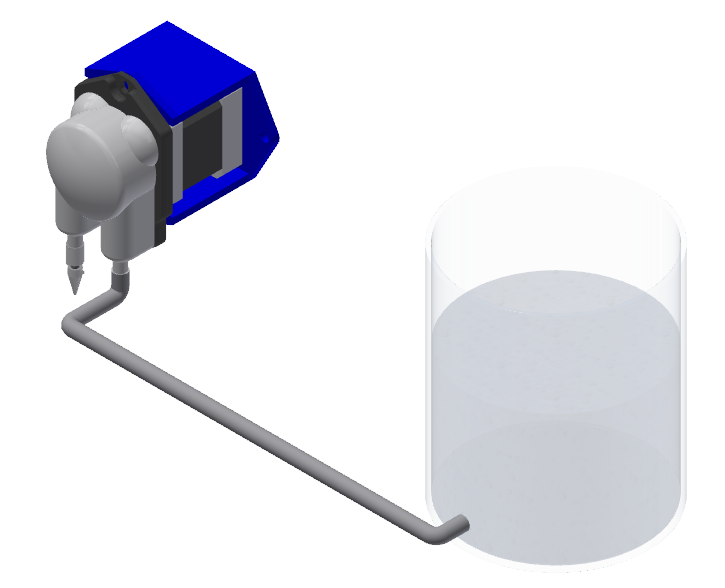
\includegraphics[scale=0.35]{figs/PumpConcept.png}
    \caption{Concept 1 Pump-Based Extruder Design}
    \label{fig:pumpConcept}
\end{figure}

\subsubsection*{Concept 2}
Figure~\ref{fig:syringeConcept1} shows the second concept that consists of an assembly of 3D printed parts, in which a stepper motor drives two lead screws (through a system of printed gears) to push a plunger further into a store-bought syringe. The pre-existing syringe is easily removable by either unbolting the flanged tube in which the syringe sits or by sliding the syringe out vertically when the platform that pushes the plunger is in its uppermost position. The inclusion of gears is used to allow the plunger to be driven with a greater force magnitude for extruding high-viscosity gels through small-diameter nozzles.

\begin{figure}[H]
    \centering
    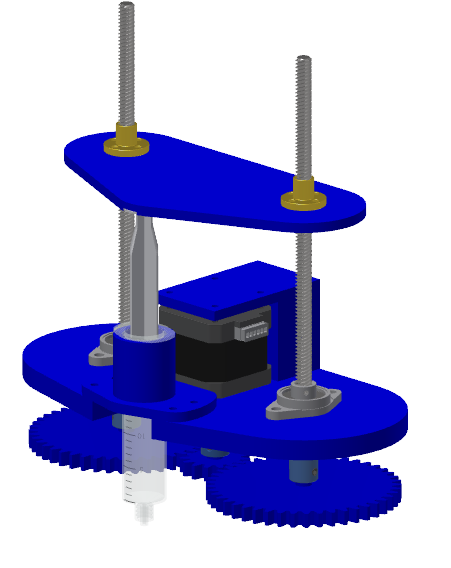
\includegraphics[scale=0.7]{figs/SyringeConcept1.png}
    \caption{Concept 2 Syringe-Based Extruder Design}
    \label{fig:syringeConcept1}
\end{figure}

\subsubsection*{Concept 3}
The final concept, in Figure~\ref{fig:syringeConcept2}, shows another syringe-based extruder like the second concept. This concept deviates from the previous one in a few ways, including its syringe, material composition, and actuation style. This concept uses a custom-made aluminium syringe with a PVC plunger and threaded nozzle to accept screw-in component additions (for added modularity). This concept is also made up of additional machined aluminium platforms. The extruder uses a GT2 belt-and-pulley drive-train to increase the force of the lead screw on the plunger and also uses a shaft to guide the plunger-driving platform.
\begin{figure}[H]
    \centering
    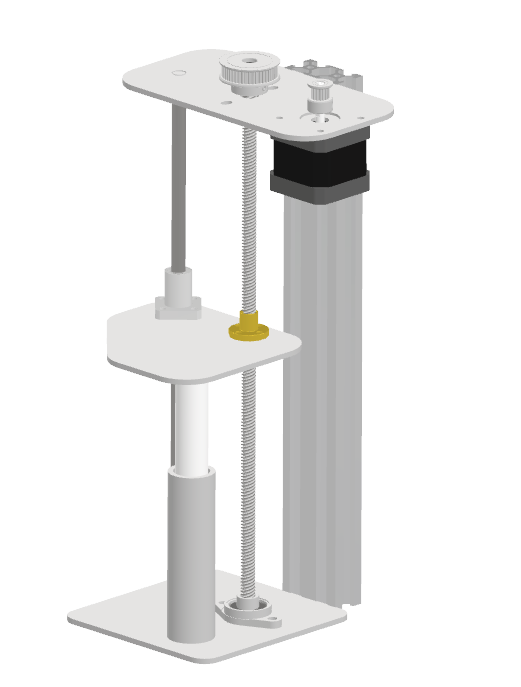
\includegraphics[scale=0.65]{figs/SyringeConcept3.png}
    \caption{Concept 3 Custom Syringe-Based Extruder Design}
    \label{fig:syringeConcept2}
\end{figure}

\subsection{Concept Evaluation and Selection}
To objectively evaluate the three generated concepts and identify the one that best satisfies the project’s stakeholder requirements, a Pugh chart was developed. This method compares each concept against multiple weighted criteria, each derived from a specific stakeholder requirement. Concept 2 was selected as the reference datum, and the other concepts were rated relative to it on a scale from –2 to +2, with positive values indicating favourable performance and negative values indicating less favourable performance. Table~\ref{tab:pugh1} presents the results of the Pugh chart evaluation.

\begin{sidewaystable}[p]
\centering
\caption{Concept Evaluation (Pugh Chart)}
\label{tab:pugh1}
\renewcommand{\arraystretch}{1.2}
\setlength{\tabcolsep}{3.5pt}

\begin{tabular}{|>{\centering\arraybackslash}p{35mm}|
                >{\centering\arraybackslash}p{15mm}|
                >{\centering\arraybackslash}p{15mm}|
                >{\raggedright\arraybackslash}p{35mm}|
                >{\centering\arraybackslash}p{15mm}|
                >{\raggedright\arraybackslash}p{35mm}|
                >{\centering\arraybackslash}p{15mm}|
                >{\raggedright\arraybackslash}p{35mm}|}
\hline
\multicolumn{2}{|c|}{\textbf{Criterion}} &
\multicolumn{2}{c|}{\textbf{Concept 1}} &
\multicolumn{2}{c|}{\textbf{Concept 2}} &
\multicolumn{2}{c|}{\textbf{Concept 3}} \\
\hline
\textbf{Description} & \textbf{Weight} &
\textbf{Rating} & \textbf{Motivation} &
\textbf{Datum} & \textbf{Motivation} &
\textbf{Rating} & \textbf{Motivation} \\
\hline
Maximum flow rate (SR1) & 0.07 & +2 & Higher throughput & 0 & Limited by lead screw & 0 & Limited by lead screw \\\hline
Maximum extrusion force (SR1) & 0.13 & -2 & Pressure drop across longer fluid path & 0 & Limited by the buckling of the plastic plunger & +2 & High due to lead screw, drive-train and aluminium syringe \\\hline
Ink storage volume (SR1) & 0.05 & +2 & Large reservoir and continuous pump action & 0 & Limited by syringe volume & 0 & Limited by syringe volume \\\hline
Flow rate accuracy (SR3) & 0.19 & -1 & Inaccurate at low speeds & 0 & Accurate due to lead screw and gear reduction & +1 & Accurate due to lead screw and drive-train \\\hline
Support multiple hydrogels (SR5) & 0.13 & -2 & Tubing limits viscous gels & 0 & Moderate viscosity acceptable & +1 & Metal path can handle highly viscous inks \\\hline
Repeatable performance (SR6) & 0.15 & -1 & Tube ageing & 0 & Variable backlash from printed gears & +2 & Low backlash from tensioning \\\hline
Sterilisability and cleanability (SR9) & 0.13 & -2 & Hard to clean long path & 0 & Removable syringe and straight path & 0 & Removable syringe and straight path \\\hline
Affordability (SR11) & 0.15 & -2 & Requires a peristaltic pump & 0 & 3D printing and standard parts & -1 & Standard parts and machined metal \\\hline
\hline
\multicolumn{2}{|l|}{\textbf{Sum of plus ratings}} &
\multicolumn{2}{c|}{4} &
\multicolumn{2}{c|}{0} &
\multicolumn{2}{c|}{6} \\\hline

\multicolumn{2}{|l|}{\textbf{Sum of minus ratings}} &
\multicolumn{2}{c|}{-10} &
\multicolumn{2}{c|}{0} &
\multicolumn{2}{c|}{-1} \\\hline

\multicolumn{2}{|l|}{\textbf{Overall total}} &
\multicolumn{2}{c|}{-6} &
\multicolumn{2}{c|}{0} &
\multicolumn{2}{c|}{5} \\\hline

\multicolumn{2}{|l|}{\textbf{Weighted total}} &
\multicolumn{2}{c|}{-1.18} &
\multicolumn{2}{c|}{0} &
\multicolumn{2}{c|}{0.73} \\\hline

\end{tabular}
\end{sidewaystable}

\FloatBarrier

The Pugh chart indicates that Concept 3 provides the most favourable balance across the weighted criteria. Its high flow rate accuracy is achieved through the use of a lead screw and drive-train, which also enables it to deliver the greatest extrusion forces. Although less affordable than a 3D-printed design, the use of machined metal components ensures these high extrusion forces can be produced without compromising structural integrity. Together, these factors enable the extruder to handle highly viscous gels with repeatable performance while maintaining sterilisability.

\subsection{Final Extruder Design}
With Concept 3 selected as the most suitable option, the concept is refined into a final extruder design that is ready for assembly. In this subsection, the extruder is specified in detail, with calculations provided to quantify its design requirements (stepper torque, pulley ratios, and plunger dimensions) and to determine its theoretical performance characteristics such as flow rate resolution. These demonstrate that the final design meets the stakeholder requirements.
\subsubsection*{Extrusion Force Calculations}
To calculate the needed stepper torque and pulley ratio, it is first necessary to describe the system characteristics and requirements. The syringe should hold roughly \SI{25}{mL} and therefore has an internal diameter of \SI{20}{mm} and a length of \SI{80}{mm}. The nozzle’s threaded shank provides attachment for an E3D hot-end assembly that can accommodate different nozzle diameters. To be conservative and to allow printing with high accuracy, the design assumes the ability to extrude through a minimum nozzle diameter of \SI{0.2}{mm} with an approximate length of \SI{20}{mm}. To ensure compatibility with multiple hydrogels, the extruder is specified to handle gels with a maximum viscosity of $10~\si{\pascal\second}$.

These assumptions are restated in Appendix~A.1, which shows, using Poiseuille’s Law, that extrusion under these edge-case conditions requires the plunger to deliver a maximum pressure of $900~\si{\kilo\pascal}$. The calculations further indicate that, to achieve this pressure over the cylinder’s cross-sectional area, the lead screw must apply approximately \SI{300}{N} of force on the plunger. This corresponds to a torque requirement of $0.638~\text{N}\cdot\text{m}$ for the TR8$\times$8 lead screw. To achieve this, a NEMA17 stepper motor with a maximum holding torque of $0.28~\text{N}\cdot\text{m}$ is used in combination with a 3:1 GT2 pulley reduction (48T:16T), increasing the maximum torque at the lead screw to $0.84~\text{N}\cdot\text{m}$. The conservative assumption of assuming a nozzle length of 20 mm and a maximum viscosity of $10~\si{\pascal\second}$ serves as a safety factor that provides protection against worst-case scenarios such as nozzle clogging.


\subsubsection*{Flow Rate Resolution}
The minimum flow rate resolution without microstepping can be determined based on the relationship between the angle of the motor shaft, lead screw pitch, and the cross-sectional area inside the syringe. Since the system uses a pulley ratio (PR) of 3:1, the lead is \SI{8}{mm}, and the motor is adjusted by $1.8^{\circ}$ per full step, the positional accuracy with which the plunger can move is:

\begin{align*}
\Delta x_{\text{Full Step}} &= \frac{\text{Lead}}{\text{PR}} \times \frac{\theta_{\text{Full Step}}}{360^{\circ}} \\
&=\frac{8.00}{3}\times \frac{1.8^\circ}{360^\circ} \\
&= 0.0133~\text{mm}/\text{step}
\end{align*}

\noindent To convert this to a volumetric resolution, this value must be multiplied by the cross-sectional area of the syringe through which the plunger slides:
$$\Delta V_\text{Full Step} =\pi \left(10 \times 10^{-3}\right)^2 (1.33 \times 10^{-5})=4.19\times10^{-9} \,\,\text{m}^3/\text{step} =\boxed{4.19~\mu\text{L}/\text{step}} 
$$
Therefore, the extruder has a minimum theoretical extrusion resolution of $4.19~\mu\text{L}$ for a full step that drives the stepper. This resolution can be further refined through microstepping.

\subsubsection*{Buckling Analysis}
The syringe plunger is made of PVC, and the minimum diameter of the plunger stem must be determined to avoid buckling under the extrusion-force edge case of \SI{300}{N}. According to \cite{callister2018materials}, the modulus of elasticity of PVC ranges from \SI{2.41}{\giga\pascal} to \SI{4.14}{\giga\pascal}. Therefore, taking the modulus of elasticity as \SI{3}{\giga\pascal} and considering that the plunger stem length is \SI{80}{mm} (to allow full range of motion in the syringe), the minimum diameter can be determined with the Euler buckling formula and the area moment of inertia for a circular cross-section:
\[
P_{cr} = \frac{\pi^{2} E I}{(K L)^{2}}, 
\quad \text{and} \quad 
I = \frac{\pi d^{4}}{64}
\]
\[
\Longleftrightarrow
\; d = \left( \frac{64 P (K L)^{2}}{\pi^{3} E} \right)^{\tfrac{1}{4}}
\]

For this derived formula for the stem’s minimum diameter, it is further noted that the design includes parts that constrain the displacement at each end of the plunger (the syringe, and a circular hole into which a load cell is mounted and the plunger end slides). These parts constrain displacement but do not fix the plunger’s angle at either end, so Euler’s effective-length factor $K$ is assumed to be 1 (pin-to-pin connection). Therefore, the minimum diameter is:
\begin{align*}
d &= \left( \frac{64 \times 300 \times (1 \times 0.080)^{2}}{\pi^{3} \times 3 \times 10^{9}} \right)^{\tfrac{1}{4}}\\
d &= 6.03~\text{mm}
\end{align*}

As an additional safety measure, the plunger stem is specified as \SI{18}{mm}, which provides a large margin against buckling. This choice also reduces machining waste on the lathe, since the plunger head must be \SI{20}{mm} in diameter to sit within the syringe tube.

\subsubsection*{Thermal Expansion Calculations}
To allow the extruder to achieve its required maximum nozzle temperature of $85\,\,^{\circ}\text{C}$ (PR7), an E3D heater block is screwed onto the syringe's threaded nozzle and a standard 0.4 mm 3D printer nozzle is screwed into the heater block. However, the ability to elevate the syringe's temperature results in the thermal expansion of some of its components. PVC has a greater coefficient of thermal expansion than aluminium, which means that the plunger requires a minimum tolerance between the plunger head's outer diameter and syringe barrel's inner diameter must be determined to prevent the heated plunger from binding inside the syringe. According to \cite{callister2018materials}, the linear coefficients of thermal expansion for 6061 aluminium alloy and PVC are $23.6\times10^{-6}$ ($\alpha_\text{Al}$) and up to \SI{180e-6}{\per\kelvin} ($\alpha_\text{PVC}$). Therefore, the minimal diametric clearance must be (assuming $T_\text{room} = 20^{\circ}\text{C}$):
\[
\Delta d_{\text{tol}} = \left( \alpha_{\text{PVC}} - \alpha_{\text{Al}} \right) d \, \Delta T = (180-23.6)(1\times10^{-6})(20)(85-20)=\boxed{0.203~\text{mm}}
\]
\subsubsection*{Final Design}
The final extruder design is shown below in Figure~\ref{fig:extruderFinal}.  
\begin{figure}[H]
    \centering
    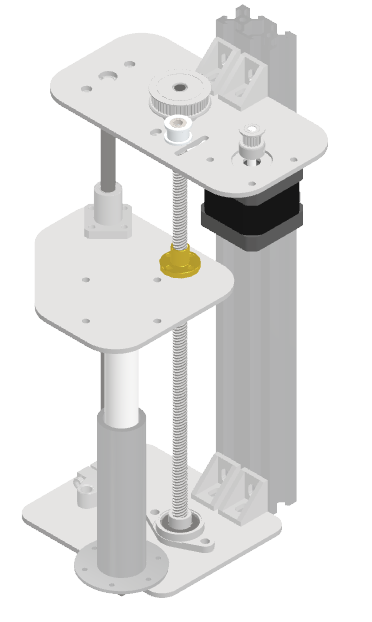
\includegraphics[scale=0.9]{figs/FinalExtruder.png}
    \caption{Final Syringe-Based Extruder Design}
    \label{fig:extruderFinal}
\end{figure}

This figure shows the refined version of Concept 3. It adds brackets to mount the platforms to the 2020 aluminium extrusion, includes a slot-and-idler-based belt tensioning mechanism, separates the syringe from the lower platform into two parts mounted together via the syringe’s flange. An E3D heater assembly is also mounted to the syringe's threaded nozzle in order to raise the temperature of the syringe.

\section{Gantry Design}
The design of a gantry enables the positioning of the extruder, allowing the system to function as a 3D printer. This section follows the same structure as the extruder design in which concepts are developed and evaluated, a single concept is selected and refined into a final design. 
\subsection{Concept Generation}
\subsubsection*{Concept 1}
The first concept (Figure~\ref{fig:Gantry1}) uses a CoreXY system with two steppers driving the XY belts and a third stepper that lifts the bed via a lead screw. The frame is made from aluminium extrusions, with linear rails guiding all horizontal motion. The Z-axis bed is guided by two shafts and bearings and the bed is comprises of a removable copper plate (to aid in manual process like curing or cleaning). 
\begin{figure}[H]
    \centering
    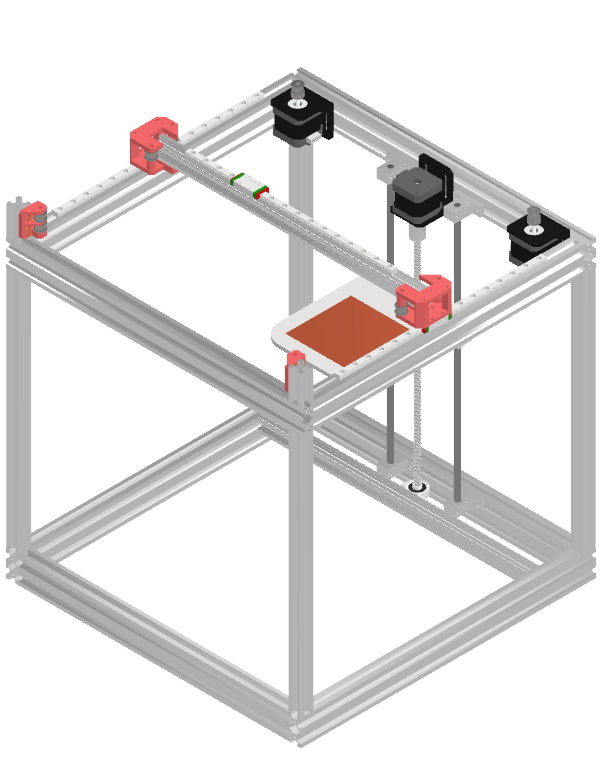
\includegraphics[scale=0.68]{figs/GantryConcept2.png}
    \caption{Concept 1 CoreXY Design}
    \label{fig:Gantry1}
\end{figure}

\subsubsection*{Concept 2}
In Figure~\ref{fig:Gantry2}, each axis is driven by its own lead screw(s) (all turned by NEMA 17 stepper motors), with wheel carriages guiding motion along aluminium extrusions. The bed is supported by two linear shafts with bearings and also has a removable copper plate. 
\begin{figure}[H]
    \centering
    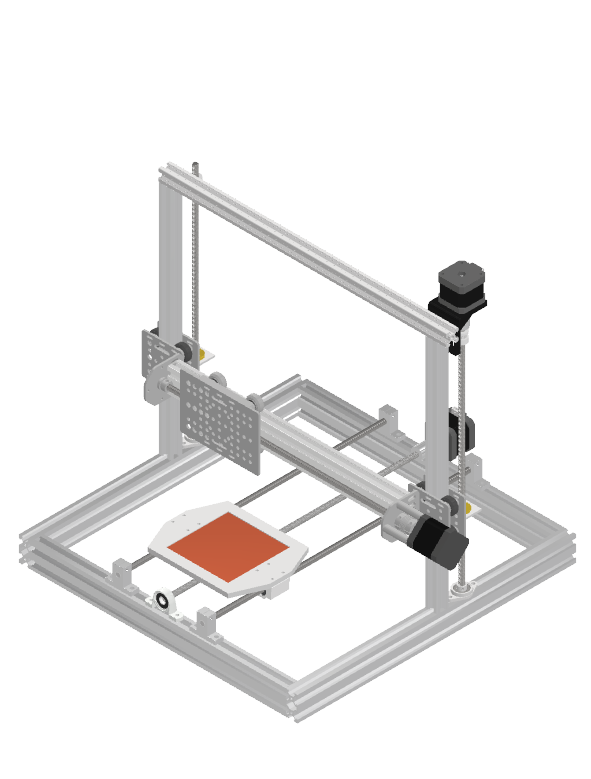
\includegraphics[scale=0.8]{figs/GantryConcept1.png}
    \caption{Concept 2 Bed-Slinger Design with only Lead Screws}
    \label{fig:Gantry2}
\end{figure}

\subsubsection*{Concept 3}
The final design, in Figure~\ref{fig:Gantry3}, uses two lead screws (synchronized by a GT2 belt), driven by one stepper, to lift the Z-axis beam. The extruder carriage is guided along the Y-axis v-slot aluminium beam and driven by a GT2 belt, while another belt drives the bed in the X-direction along two rods (like in Concept 2). The bed is a fixed aluminium plate to enable the addition of a permanent cooling mechanism (Peltier).
\begin{figure}[H]
    \centering
    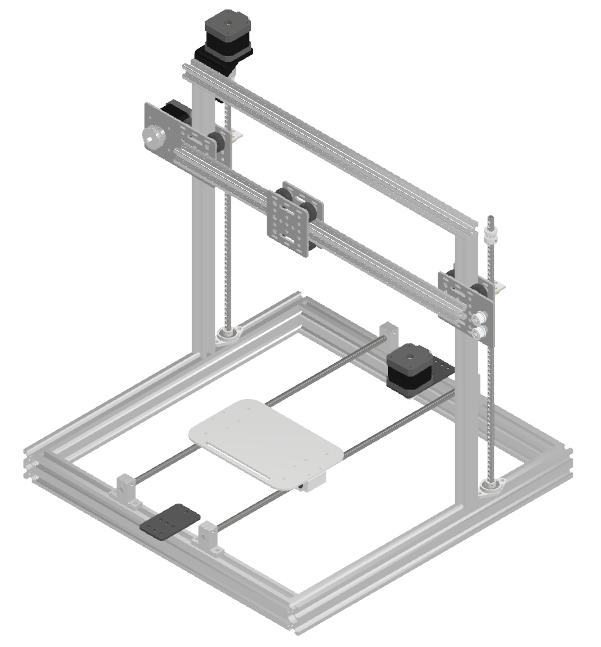
\includegraphics[scale=1]{figs/Gantry3.png}
    \caption{Concept 3 Bed-Slinger Design with Lead Screws and Belts}
    \label{fig:Gantry3}
\end{figure}

\subsection{Concept Evaluation and Selection}
The previously generated concepts are evaluated, as was done with the design of the extruder, with the purpose of selecting the concept that best satisfies the project’s stakeholder and engineering requirements. The evaluation is carried out in Table~\ref{tab:pugh2}, which compares each concept against a set of weighted criteria (based on the project's stakeholder requirements). These criteria include factors such as positional accuracy, speed, affordability, and sterilisability. Each factor was compared against Concept 2 (the datum) using a relative score of up to $\pm2$ (as with the extruder evaluation). The resulting scores were then totalled according to each criterion’s respective weight.
\begin{sidewaystable}[p]
\centering
\caption{Concept Evaluation (Pugh Chart)}
\label{tab:pugh2}
\renewcommand{\arraystretch}{1.2}
\setlength{\tabcolsep}{3.5pt}
\begin{tabular}{|>{\centering\arraybackslash}p{35mm}|
                >{\centering\arraybackslash}p{15mm}|
                >{\centering\arraybackslash}p{15mm}|
                >{\raggedright\arraybackslash}p{35mm}|
                >{\centering\arraybackslash}p{15mm}|
                >{\raggedright\arraybackslash}p{35mm}|
                >{\centering\arraybackslash}p{15mm}|
                >{\raggedright\arraybackslash}p{35mm}|}
\hline
\multicolumn{2}{|c|}{\textbf{Criterion}} &
\multicolumn{2}{c|}{\textbf{Concept 1}} &
\multicolumn{2}{c|}{\textbf{Concept 2}} &
\multicolumn{2}{c|}{\textbf{Concept 3}} \\
\hline
\textbf{Description} & \textbf{Weight} &
\textbf{Rating} & \textbf{Motivation} &
\textbf{Datum} & \textbf{Motivation} &
\textbf{Rating} & \textbf{Motivation} \\
\hline
% ---- Rows: duplicate as needed ----
Maximum XY speed (SR1) & 0.12 & +1 &  Uses belts & 0 & Limited by lead screw & +1  & Belts can achieve higher speeds \\\hline
XY positional accuracy (SR2) & 0.24 & -1 & Belts are less accurate & 0 & High accuracy of lead screws & -1 & Belts are less accurate \\\hline
Z positional (layer height) accuracy (SR2) & 0.24 & -1 & Uses lead screws but is susceptible to bending & 0 & Accurate due to lead screws & 0 & Accurate due to lead screws \\\hline
Sterilisability and cleanability (SR9) & 0.20 & 0 & Removable copper bed & 0 & Removable copper bed & -1 & Fixed bed \\\hline
Affordability (SR11) & 0.20 & -1 & Requires more parts (Idlers and tensioners) & 0 & Uses more expensive parts (lead screws compared to belts) & +2 & Simplest build with cost effective, standard parts \\\hline
% ---- Summary rows ----
\hline
\multicolumn{2}{|l|}{\textbf{Sum of plus ratings}} &
\multicolumn{2}{c|}{1} &
\multicolumn{2}{c|}{0} &
\multicolumn{2}{c|}{3} \\\hline

\multicolumn{2}{|l|}{\textbf{Sum of minus ratings}} &
\multicolumn{2}{c|}{-3} &
\multicolumn{2}{c|}{0} &
\multicolumn{2}{c|}{-2} \\\hline

\multicolumn{2}{|l|}{\textbf{Overall total}} &
\multicolumn{2}{c|}{-2} &
\multicolumn{2}{c|}{0} &
\multicolumn{2}{c|}{1} \\\hline

\multicolumn{2}{|l|}{\textbf{Weighted total}} &
\multicolumn{2}{c|}{-0.56} &
\multicolumn{2}{c|}{0} &
\multicolumn{2}{c|}{0.08} \\\hline

\end{tabular}
\end{sidewaystable}
\FloatBarrier

\noindent The results of Table~\ref{tab:pugh2}'s evaluation reveal that Concept 3 is the most suitable option of the three generated concepts, achieving the highest overall weighted score and therefore best satisfies the system's stakeholder requirements. While it is more difficult to clean/sterilise the bed after prints due to it being fixed to the linear bearings, it provides a base to mount a Peltier module for bed cooling which would not have been practical if the bed was removable. It also performs favourably in terms of speed and affordability, due to its use of standard GT2 belts that are often used in 3D printing. It can also achieve high layer height accuracy due to its use of synchronised lead screws. 

\subsection{Final Gantry Design}
Finally, Concept 3, needs to be refined and developed into a final gantry design that is ready for procurement and assembly.

\subsubsection*{Z Axis Stepper Requirements and Positional Accuracy}
To determine the stepper torque requirements, the mass driven by the synchronised lead screws must be approximated. This can be done using Inventor Professional’s iProperties feature, which revealed that the total volume of the portion of the final design (extruder, horizontal beam, motors, and carriages) being lifted in the Z-direction is \SI{688658.130}{\milli\meter^3}. By assuming the average density of this assembly is \SI{2.7e-6}{\kilogram\per\milli\meter^{3}} (the density of aluminium), the mass to be moved by the lead screws is approximated as \SI{1.86}{\kilogram}. 

Appendix A.2, using the same lead screw properties as A.1, shows that this requires a minimum stepper torque of \SI{0.0388}{\newton\meter}. The final design uses a Creality 42-40 Stepper Motor that is capable of a holding torque of up to \SI{0.4}{\newton\meter}. The lead screw torque therefore has a safety factor of roughly 10 to allow for the system to achieve high accelerations along the Z-axis.

Finally, the positional accuracy of the Z-control must be characterised. The chosen stepper has a step angle of $1.8^\circ$ and the TR8x8 lead screws have a lead of \SI{8}{mm}. Therefore the positional resolution is:
\begin{align*}
\Delta z_{\text{Full Step}} &= \text{Lead} \times \frac{\theta_{\text{Full Step}}}{360^{\circ}} \\
&=8.00\times \frac{1.8^\circ}{360^\circ} \\
&= 0.04~\text{mm}/\text{step}
\end{align*}

\noindent This theoretical accuracy exceeds the \SI{50}{\micro\meter} requirement established in PR3. It should be noted that an even higher resolution can be achieved with microstepping.

\subsubsection*{X and Y Axis Stepper Requirements and Positional Accuracy}
Autodesk Inventor Professional can be used to reveal the final extruder has a total volume of \SI{379353.531}{\milli\meter^3} and the printer bed with its linear bearings, heat sink, Peltier and cold plate (shown in the final design later in Figure~\ref{fig:gantryFinal}) has a total volume of \SI{145105.084}{\milli\meter^3}. As done previously, by multiplying these volumes by the density of aluminium (\SI{2.7e-6}{\kilogram\per\milli\meter^{3}}), yielding two separate mass approximations of \( m_x = 0.39\,\text{kg} \) and \( m_y = 1.02\,\text{kg}\). By further assuming the carriages' friction coefficient to be 0.2 and the maximum horizontal acceleration to be \( a = 5\,\text{m/s}^2 \), the required stepper torque can be determined for each axis, as shown in Appendix A.3. The X-axis uses a GT2 pulley with 20 teeth and the calculations show that the stepper requires $0.0173\,\text{Nm}$ of torque and the Y-axis stepper (which uses a 36 teeth pulley) needs $0.08137\,\text{Nm}$. Therefore, the chosen NEMA 17 steppers have a holding torque up to \SI{0.28}{\newton\meter} for the X-axis and \SI{0.4}{\newton\meter} for the Y-axis.

With these described specifications, the positional accuracy in horizontal plane can be determined. Considering the use of pulleys in both the X and Y directions, the resolution can determined by multiplying the motors step angle with the radius of each pulley ($r_x=6.365$ and $r_y=11.46$):
\begin{align*}
    \Delta x &= \theta_{\text{Full Step}}\times r_x=1.8^\circ\frac{\pi}{180^\circ}\times6.365=0.200\,\text{mm}\\
    \Delta y &=\theta_{\text{Full Step}}\times r_y=1.8^\circ\frac{\pi}{180^\circ}\times11.46=0.360\,\text{mm}
\end{align*}
These fall short of the target set in PR2, but both fall within the acceptable range. However, they can be configured to meet the target by using the drivers to enable microstepping of at least 1/4.
\subsubsection*{Final Gantry}

\begin{figure}[H]
    \centering
    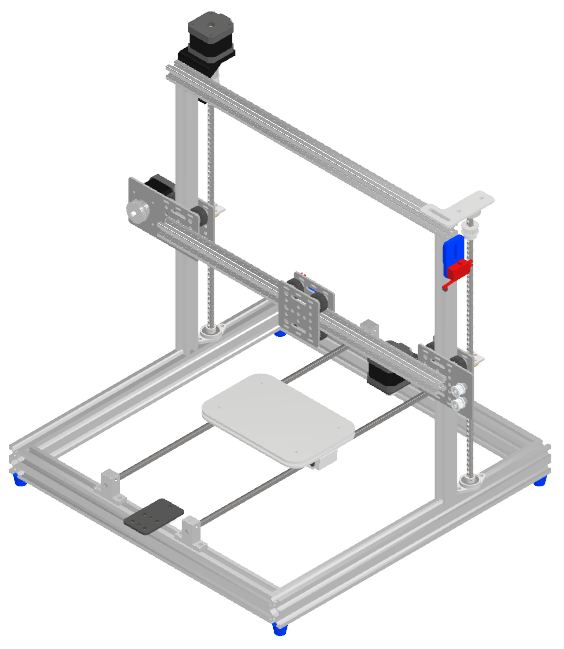
\includegraphics[scale=0.8]{figs/FinalGantry.png}
    \caption{Final Bed-Slinger Gantry Design}
    \label{fig:gantryFinal}
\end{figure}
The final gantry design is shown above in Figure~\ref{fig:gantryFinal}. It is the refined design, based on Concept 3, and incorporates a Peltier cooler mounted to the bed between two plates (cold side on top and heat sink at the bottom). The figure also shows the system's limit switches for homing.
\section{Final Design}
\noindent
The complete bioprinter design, shown in Figure~\ref{fig:bioprinterCAD}, shows the extruder and gantry subsystems, integrated into a single mechanical system. The extruder is designed to use a custom syringe, heater block, and load cell to deposit viscous gels at a controlled flow rate and temperature, while the gantry accurately positions it in 3D space to enable it to print three dimensional scaffolds. This final design concludes the mechanical design of the project and forms the basis for the embedded systems design and integration to enable the printer to function as required and undergo experimental validation.

\begin{figure}[H]
    \centering
    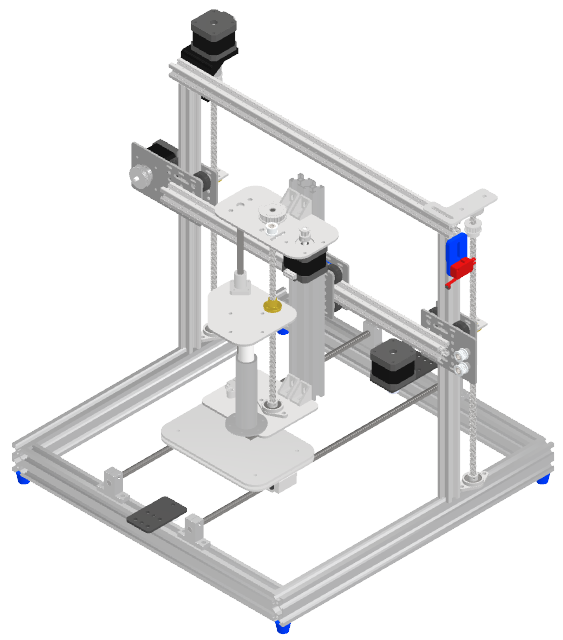
\includegraphics[scale=1]{figs/FinalBioprinter.png}
    \caption{Final Bioprinter Design}
    \label{fig:bioprinterCAD}
\end{figure}
\chapter{Embedded System Design}
This chapter details the design and implementation of the embedded control system for the hydrogel bioprinter. The embedded system is responsible for coordinating the mechatronic system’s core functions, including stepper movement, memory management, bed and nozzle temperature control, and UV curing. The electronic hardware design takes the form of a custom PCB featuring an STM32F407VGT6 microcontroller, which executes the developed firmware to allow the printer to function. While more affordable alternatives exist, the STM32F407VGT6 was selected based on prior experience, thereby reducing development time and the learning curve.

The embedded system was designed to meet the following requirements, developed for the electronic design in order to allow the whole system to meet the stakeholder requirements from chapter 3:

\begin{itemize}
    \item The system must safely supply regulated 3.3 V to the logic subsystems from a 12 V DC power supply that plugs into a standard wall socket.
    \item The system must be able to drive up to five stepper motors through A4988 driver breakout modules.
    \item The system must be able to receive real-time sensor data, including extrusion force from a load cell and temperature readings from thermocouples.
    \item The device must implement switching control for a heater cartridge, Peltier module, UV curing light, and cooling fan.
    \item The system is required to receive print task via a microSD card.
    \item The printer must implement feedback control loops for extrusion pressure and temperature regulation.
    \item The system must provide headers for unused controller pins to support future upgrades.
\end{itemize}


The final assembled hydrogel bioprinter, including the implemented embedded system, is shown below in Figure~\ref{fig:FinalPrinter}:
\begin{figure}[H]
    \centering
    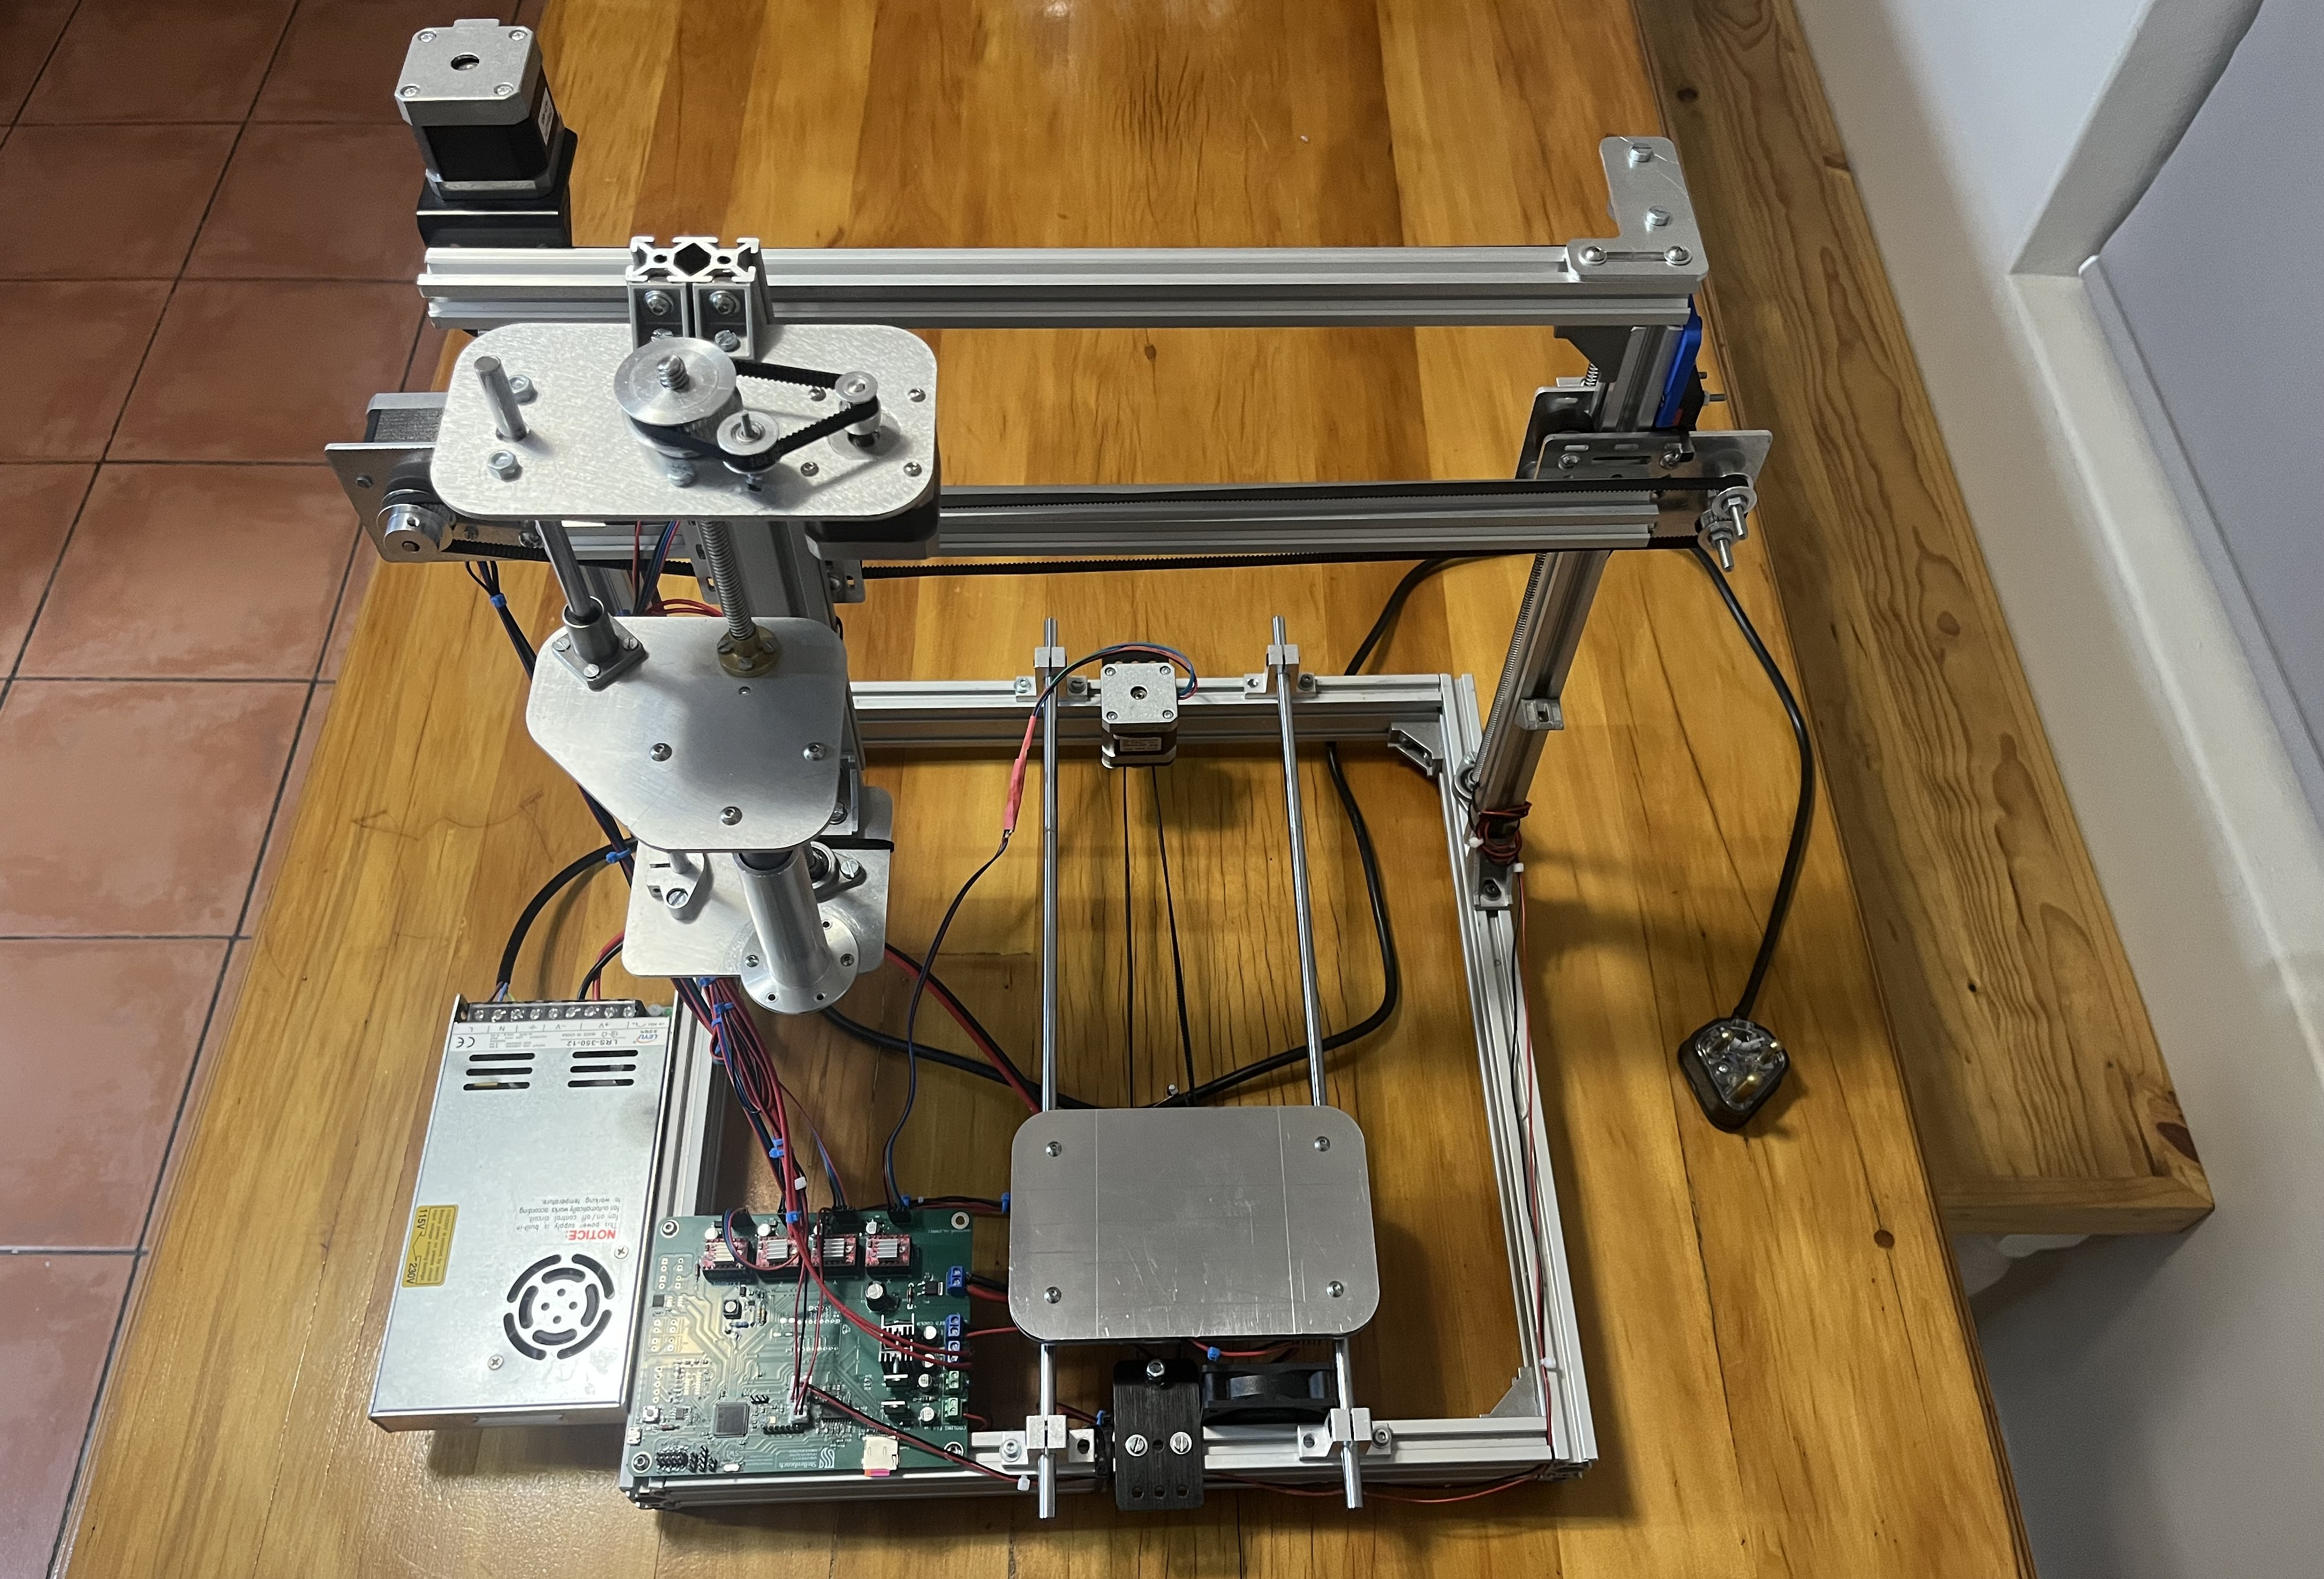
\includegraphics[scale=0.1]{figs/AssembledSystemView.jpg}
    \caption{The Final Assembled Hydrogel Bioprinter}
    \label{fig:FinalPrinter}
\end{figure}

\section{System Description}
The embedded system as a whole enables the printer's automated operation. It is powered by a 12 V PSU that directly supplies power to the stepper drivers, Peltier module, UV curing light, heater cartridge, and cooling fan. The 12 V is also converted into a regulated 3.3 V source via a buck converter to power the logic circuits. The STM32 controller reads print instructions from a microSD card so that it can then control the stepper motors (through drivers) using an ISR. During stepper operation, system information is transmitted to a laptop via a USB connection for external monitoring. External peripherals (Peltier, heater cartridge, cooling fan, and curing light) are connected to the 12 V source and switched between their ON and OFF states using N-channel power MOSFETs.

This description of the system is visually represented in the block diagram below in Figure~\ref{systemblockdiagram}. The black arrows represent the logic flow, the red arrows show the 12 V power distribution, and the green arrow shows how the 3.3 V power source is distributed.
    
\begin{figure}[H]
\centering
\begin{tikzpicture}[
  voltagecircle/.style = {circle, draw=black, thick, minimum size=1.2cm, align=center},
  block/.style = {rectangle, draw=black, thick, minimum width=3.5cm, minimum height=1cm, align=center},
  mcu/.style = {rectangle, rounded corners=5pt, draw=black, thick, minimum width=1cm, minimum height=3cm, align=center, fill=white},
  lp/.style = {rectangle, rounded corners=5pt, draw=black, thick, minimum width=1cm, minimum height=1.5cm, align=center, fill=white},
  io/.style = {rectangle, rounded corners=5pt, draw=black, thick, minimum width=2.5cm, minimum height=1cm, align=center},
  arrow/.style = {thick, -{Latex[scale=1.2]}},
  arrow2/.style = {thick, -{Latex[scale=1.2]}, color=red},
  arrow3/.style = {thick, -{Latex[scale=1.2]}, color=green}
]

% Power supply chain
\node[voltagecircle] (src) at (0.45, 8.5) {12 V\\Source};
\node[block] (reg3v3) at (5, 8.5) {3.3 V Regulator};
\node[mcu] (mcu) at (5, 4) {STM32F407\\MCU};
% Right
\node[io] (switch) at (9.2, 7.5) {Limit Switches};
\node[io] (temp) at (9.8, 6) {Temperature Sensors};
\node[io] (load) at (10, 4.5) {Extrusion Force Sensor};
\node[io] (eeprom) at (9.1, 3) {EEPROM};
\node[io] (sdcard) at (9.3, 1.5) {microSD Card};
% Left
\node[io] (step) at (0.45, 4.5) {Stepper Drivers};
\node[io] (fet) at (0, 3) {Switching MOSFETs};
% Bottom
\node[io] (usb) at (5, 1.5) {USB connection};
\node[lp] (laptop) at (0, 1.5) {Laptop};
% 12V Power flow arrows
\draw[arrow2] (src.east) -- (reg3v3.west);
\draw[arrow2] (src.south) -- (step.north);
\draw[arrow2] (0.45, 5.5) -- (-1.5, 5.5) -- (-1.5, 3.5);
% 3v3 Power flow arrows
\draw[arrow3] (reg3v3.east) -- (13,8.5) -- (13,1.5) -- (sdcard.east);
\draw[arrow3] (13,3) -- (eeprom.east);
\draw[arrow3] (13,4.5) -- (load.east);
\draw[arrow3] (13,6) -- (temp.east);
\draw[arrow3] (reg3v3.south) -- (mcu.north);
\draw[arrow3] (5,6) -- (1.5,6) -- (1.5,5);
% Logic flow arrows
\draw[arrow] (mcu.south) -- (usb.north);
\draw[arrow] (usb.west) -- (laptop.east);
\draw[arrow] (switch.west) -- (5.7,7.5) -- (5.7, 5.49);
\draw[arrow] (temp.west) -- (6.7,6) -- (6.7, 5) -- (6.2, 5);
\draw[arrow] (load.west) -- (6.2,4.5);
\draw[arrow] (eeprom.west) -- (6.25, 3);
\draw[arrow] (6.25, 3) -- (eeprom.west);
\draw[arrow] (sdcard.west) -- (6.9,1.5) -- (6.9, 2.7) -- (6.2, 2.7);
\draw[arrow] (3.77, 4.5) -- (step.east);
\draw[arrow] (3.77, 3) -- (fet.east);

\end{tikzpicture}
\caption{System Block Diagram of the Bioprinter's Embedded System}
\label{systemblockdiagram}
\end{figure}

\section{Hardware Design and Implementation}
The hardware design, as previously stated, took place in the form of a custom PCB. The PCB was designed using KiCad and manufactured by JLCPCB. The electronic system can be separated into various subsystems, including the power supply, stepper drivers, limit switches, memory handling circuit, load cell sensing circuit, temperature reading circuit, and the N-channel MOSFET switching circuit. The timing of each subsystem is coordinated by a high-speed crystal oscillator. A schematic overview of the PCB is shown in Figure~\ref{fig:pcb_overview} in Appendix C.


\subsection{Power Supply}
The power supply subsystem, shown in Figure~\ref{fig:pcb_power}, incorporates both circuit protection and voltage conversion through a buck converter. The printer is powered by a 350 W LRS PSU, which allows direct connection to a standard wall socket and converts the municipal 230 $V_{\text{RMS}}$ supply into a regulated 12 V DC output. This output is delivered to the PCB via screw terminals. 

In the event of incorrect wiring, the system makes use of reverse polarity protection using a high-side P-channel MOSFET. This ensures that, if the ground and 12 V connection are swapped, the source output is 0 V instead of -12 V. This method was chosen over a simple series diode to eliminate forward voltage drop and preserve the full 12 V for the stepper drivers and switching peripherals. 

The entire circuit board also uses bulk and decoupling capacitors to filter out a wide range of frequencies to produce stable voltage levels for both 12 V and 3.3 V components. The 12 V source also makes use of TVS diodes (SMAJ16A) positioned near inductive loads, such as the buck converter, stepper drivers, and cooling fan port, to suppress transient voltage spikes.

This subsystem also has the role of producing a stable 3.3 V source for the logic circuitry. To do this, the PCB uses an AP3211 buck converter, following the typical \SI{12}{V} to \SI{3.3}{V} application circuit by \cite{AP3211}.
\subsection{Power Debug LEDs}
The electronic hardware incorporates debug LEDs to show the presence of specific voltage levels. A green LED ($V_f \approx$\SI{2}{V}) is connected to the buck converter's 3.3 V output to confirm that the system is connected to power and that the input voltage is successfully converted to 3.3 V. A second debug LED, a blue LED ($V_f \approx$\SI{3}{V}), is connected to the USB port's 5 V pin to show when the board is connected to a laptop via USB. Both LEDs require current limiting resistors, which were calculated to limit the current to 10 mA as follows:
\begin{align*}
R_{3.3\text{V}} = \frac{3.3\ \text{V} - 2.0\ \text{V}}{10\ \text{mA}}
= 130\ \Omega
\,\,\,\,\,\,\,\,\,\,\, \text{ and } \,\,\,\,\,\,\,\,\,\,\,
R_{5\text{V}} = \frac{5.0\ \text{V} - 3.0\ \text{V}}{10\ \text{mA}}
= 200\ \Omega.
\end{align*}
For an added safety margin, \SI{220}{\ohm} resistors were used for both LEDs.

\subsection{Stepper Driver Interface}
To interface with the stepper motors, the PCB employs five A4988 driver modules, as shown in Figure~\ref{fig:pcb_steppers}. Three drivers control the motors of the 3-axis gantry, one drives the extruder stepper, and one spare driver is included to allow future upgrades, such as the addition of a second extruder. The A4988 drivers come in the form of Pololu breakout modules that plug into female headers on the PCB (visible in the 3D model in Appendix B.9). The advantage of using socketed breakout drivers is that they can be easily replaced in the event of damage. The headers follow the StepStick form factor which means the A4988 drivers can be replaced with more advanced drivers such as the TMC2209. While each driver requires a dedicated GPIO pin for its STEP and DIR inputs, to conserve controller pins, the $\overline{En}$, $\overline{SLEEP}$, $\overline{RESET}$, and the microstepping setting pins (M0, M1, and M2) are shared across all five drivers.

To limit the current, the potentiometer on each stepper driver needs to be adjusted to reach a desired reference voltage which can be obtained using the following formula: 
\[
I_{\text{limit}} \;=\; \frac{V_{\text{ref}}}{8 R_{\text{sense}}}
\qquad\Longleftrightarrow\qquad
V_{\text{ref}} \;=\; 8R_{\text{sense}}\cdot I_{\text{limit}}.
\]

By looking at the drivers and checking the stepper motor specifications, it can be concluded that:
\begin{itemize}
    \item \(R_{\text{sense}} = 0.10~\Omega\)
    \item \(I_{\text{limit}} = 1.0~\text{A}\)
\end{itemize}

\[V_{\text{ref}} \;=\; 8\cdot 0.10\cdot 1.0=0.8\text{ A.}\]

\subsection{Limit Switches}
Figure~\ref{fig:pcb_overview} shows that the circuit board provides four limit switch connection points. Only three are utilised to allow for the homing of each gantry axis. The COM pin of each limit switch is connected to ground and the NO pin is connected to a dedicated GPIO input pin (PC0-PC2) that is pulled high so that when each axis reaches the end of its range of motion, the switch gets triggered and is pulled low.
\subsection{Memory and Connectivity Interfaces}
The board employs various means of handling memory and connecting with external devices, both for reading and transmitting data as well as for programming and debugging. This functions are achieved through the inclusion of an EEPROM, a microSD port, a USB port, and an SWD interface (Figure~\ref{fig:pcb_overview}).


The controller is connected to an M24C64 EEPROM, which provides a means of storing non-volatile information via an \(I^2C\) connection, ensuring that data can be retained even after the printer’s power source is disconnected. In addition to this, the circuit board incorporates a microSD card port for reading print task files through the MCU’s SPI1 channel. A USB port is also included, allowing the board to connect to a laptop and transmit live data—such as temperature and extrusion force readings for external monitoring and analysis. Because the USB interface requires a highly accurate clock speed (48 MHz) for reliable data transmission, the PCB includes a 16 MHz external crystal oscillator to provide a precise reference for the phase-locked loop \citep{ST_STM32F405F407_datasheet}.

For programming and debugging, the board includes a 2×5 male header array. Each pin in the header is connected to the relevant system points, including the 3.3 V supply, ground, and the required STM32 pins (SWDIO, SWCLK, SWO, and NRST). During development, these SWD pins were connected to the corresponding pins of an STM32F407G-DISC1 development board to enable programming and debugging via its integrated ST-Link interface.

To improve modularity and support future upgrades, the board includes expansion headers that connect to unused MCU pins (Figure~\ref{fig:pcb_power}). These pins connect to spare GPIO, ADC, USART, \(I^2C\), and SPI channels, enabling potential additions such as external displays.

\subsection{Load Cell Circuit}
Figure~\ref{fig:pcb_sensors} shows the circuits sensor system which includes extrusion force sensing using a load cell amplifier. The amplifier circuit design was based on the SparkFun open-source HX711 load cell amplifier breakout module \citep{SparkFunHX711}. This is powered by the board's 3.3 V supply and connected to two controller GPIO pins (a clock pin and an input pin). The board has four relevant screw terminal connection points for an external load cell (RED, BLACK, WHITE, and GREEN).

The 50 kg load cell used to measure the extrusion force is configured as a half Wheatstone bridge (containing two \SI{1}{\kilo\ohm} resistors). To form a complete Wheatstone bridge, two additional \SI{1}{\kilo\ohm} resistors are required, as shown in the full load cell–to–PCB set-up in Figure~\ref{fig:loadcell}.
\begin{figure}[H]
\centering
\begin{tikzpicture}[
  block/.style = {rectangle, draw=black, thick, minimum width=1.2cm, minimum height=0.8cm, align=center},
  lc/.style = {rectangle, rounded corners=5pt, draw=black, thick, minimum width=2.5cm, minimum height=3cm, align=left},
  pcb/.style = {
  rectangle, rounded corners=5pt, draw=black, thick,
  text width=4cm,            % content width
  inner xsep=8pt, inner ysep=20pt,
  align=left
  },
  arrow/.style = {thick, -{Latex[scale=1.2]}}
]

% Power supply chain
\node[lc] (loadcell) at (0, 0) {50 kg\\ Load Cell};
\node[pcb] (board) at (10,0.3) {RED \\[10pt] BLACK \\[10pt] WHITE \\[10pt] GREEN};
\node[block] (res1) at (4, 1) {\SI{1}{\kilo\ohm}};
\node[block] (res2) at (4, 0) {\SI{1}{\kilo\ohm}};
% connections
\draw (1.25,-1) -- (7.73,-1);
\draw (1.25, 0) -- (3.4,0);
\draw (1.25, 1) -- (3.4,1);
\draw (4.6, 1) -- (5,1) -- (5,-0.1) -- (7.73,-0.1);
\draw (4.6, 0) -- (5,0);
\draw (2.7,0) -- (2.7,0.75) 
      arc[start angle=-90,end angle=90,radius=0.25cm] -- (2.7,1.7) -- (5.3,1.7) -- (5.3,0.7) -- (7.73,0.7);
\draw (2,1) -- (2,2) -- (5.6,2) -- (5.6,1.6) -- (7.73,1.6);

\node at (7.2,1.8) {E+};
\node at (7.1,0.9) {E-};
\node at (7.1,0.1) {A-};
\node at (7.2,-0.8) {A+};
\end{tikzpicture}
\caption{Load Cell Setup}
\label{fig:loadcell}
\end{figure}

\subsection{Thermocouple Circuit}
The temperature sensing circuit is shown in Figure~\ref{fig:pcb_sensors}. This uses a MAX6675 K-type thermocouple, which is connected to the STM32's SPI2 pins (PB12-PB14). The amplifier receives the analogue thermocouple input, converts the signal into a digital value, and outputs this to the controller via the Serial Peripheral Interface. 

To allow the controller to read multiple thermocouples using a single amplifier, an analogue multiplexer (TMUX1208) is used. The MUX cycles through eight two-pin thermocouple screw terminals, where the T+ line connects to the amplifier input and the T– line is tied to ground. Channel selection is controlled by the MUX’s enable pin (EN) and three select pins (A0, A1, A2). The binary combination of these pins determines which of the eight thermocouple channels is connected to the amplifier input at a given time.

\subsection{FET Switching Circuit}
Figure~\ref{fig:pcb_control} shows the control circuit responsible for switching the system's various 12 V peripherals. These 12 V peripherals (each connected via two-pin screw terminals), include a Peltier cooling module, an E3D heater cartridge, a cooling fan, and a UV curing light. For safety reasons and due to the use of a non-curable surrogate gel in the experimental procedure (described in Chapter 5), a blue led was used in place of the UV light to demonstrate functionality. 

The peripherals are switched using N-Channel power MOSFETs (IRLZ44N), which are capable of handling high currents required by components such as the Peltier module (maximum current 7 A). The transistors are configured as low-side switches, with their source terminals tied to ground, drains connected to the negative side of the loads, and gates driven by STM32 GPIO outputs. If fully implemented, a UV light would be kept in a fixed position and flood the print bed with an adjustable intensity, which would be set by a duty cycle read from the microSD card during print commands.

A potential issue with this arrangement is that the transistor gates act as capacitive loads. When GPIO outputs transitions from high to low, the stored charge from the gate capacitance discharges into the MCU pin as a temporary transient discharge current. Since each GPIO pin is only rated for 25 mA \citep{ST_STM32F405F407_datasheet}, this risks damaging the controller. To mitigate this, small series resistors are placed at each gate to limit the initial discharge current.  In addition, an octal bus transceiver (SN74HC245DWR) is used as a protective buffer stage between the MCU and the MOSFET gates. This configuration not only shields the microcontroller from harmful transient currents but also improves signal integrity when driving multiple high-capacitance gates.

\subsection{PCB Design}
The embedded hardware was implemented on a custom PCB designed in KiCad and fabricated by JLCPCB. Its design required a number of engineering decisions regarding trace widths, layer count, and overall routing strategy.

The PCB is a two-layer board, with the bottom copper layer serving primarily as a ground plane and the top layer carrying power and signal routes. The complete board layout is shown in Figures~\ref{fig:pcb_3d_view} to~\ref{fig:pcb_bottom_layer}. In areas supplying the 12 V peripherals, such as the switching MOSFETs and stepper drivers, the top copper includes solid planes to provide sufficient current capacity while minimizing temperature rise.

Signal routing on the top layer generally uses 0.3 mm traces, while 3.3 V power lines were widened to 0.5 mm. The 0.5~mm trace width is justified through the empirically derived IPC-2221 current-temperature relationship, to estimate a minimum width (W) of a 1~oz/$ft^2$ thick copper trace to conduct the maximum buck-converter output current of 1.5~A with a $5~^\circ$C temperature rise:
\[
W = \frac{1}{t_{\text{cu}}}\left(\frac{I}{k(\Delta T)^{0.44}}\right)^{\frac{1}{0.725}} = \frac{1}{1.378}\left(\frac{1.5}{0.048(5)^{0.44}}\right)^{\frac{1}{0.725}} = 16.9~\text{mil} = 0.43~\text{mm}.
\]


Communication traces connecting the SD card, EEPROM, USB interface, MAX6675 thermocouple amplifier, and HX711 load cell amplifier to the STM32 microcontroller were deliberately kept short and closely routed to the MCU, with spacing between traces maximised (as far as reasonably possible) to preserve signal integrity. Similar care was taken around the buck converter circuitry to minimize interference arising from its high-frequency operation.

\section{Software Design and Implementation}
The firmware governs the 3D printer's operation. After initialising its peripherals, the system homes the gantry to its reference position and zeros the coordinate axes. It then enters an interrupt-driven routine that handles all stepper motion while the main loop cycles through system tasks such as SD card reading, USB transmission, and MOSFET duty cycle updates. The system's general software flow is visually represented in Figure~\ref{softwareflowdiagram}.

\begin{figure}[H]
\centering
\begin{tikzpicture}[
  circ/.style = {circle, draw=black, thick, minimum size=1.2cm, align=center},
  block/.style = {rectangle, draw=black, thick, minimum width=3.5cm, minimum height=1cm, align=center},
  io/.style = {rectangle, rounded corners=5pt, draw=black, thick, minimum width=2.5cm, minimum height=1cm, align=center},
  arrow/.style = {thick, -{Latex[scale=1.2]}}
]

\node[circ] (power) at (11, 5) {Power\\On};
\node[io] (sysInit) at (7.5, 5) {Initialize\\System};
\node[io] (home) at (3.5, 5) {Home};
\node[io] (zero) at (0, 5) {Zero\\Coordinates};

\node[io] (isr) at (3, 3.4) {Interrupt Service Routine};
\node[io] (step) at (8, 3.4) {Move Steppers};

\node[io] (queue) at (3, 1.7) {Add Task To\\ISR Queue};


\node[circ] (while) at (0, 0) {While\\Loop};
\node[io] (sd) at (3, 0) {Read\\SD Card};
\node[io] (fet) at (6, 0) {Update\\MOSFETs};
\node[io] (usb) at (9, 0) {USB\\Transmit};
\node[circ] (end) at (11.7, 0) {End of\\Loop};

% Logic flow arrows
\draw[arrow] (power.west) -- (sysInit.east);
\draw[arrow] (sysInit.west) -- (home.east);
\draw[arrow] (home.west) -- (zero.east);
\draw[arrow] (zero.south) -- (while.north);
\draw[arrow] (while.east) -- (sd.west);
\draw[arrow] (sd.east) -- (fet.west);
\draw[arrow] (fet.east) -- (usb.west);
\draw[arrow] (usb.east) -- (end.west);

\draw[arrow] (isr.east) -- (step.west);
\draw[arrow] (0, 3.4) -- (isr.west);

\draw[arrow] (sd.north) -- (queue.south);
\draw[arrow] (queue.north) -- (isr.south);
\end{tikzpicture}
\caption{Bioprinter's Generalised Software Flow Diagram}
\label{softwareflowdiagram}
\end{figure}

\subsection{Homing}
Upon startup, after all system peripherals have been initialised, the printer performs a homing sequence in which the gantry moves each of its three axes towards known reference positions (0, 0, 0). This procedure establishes the origin of the its coordinate system, ensuring that its absolute extruder position for a given coordinate remains consistent between power cycles.

The A4988 drivers are enabled (EN low, RESET and SLEEP high) and configured for 1/16 microstepping (M0,M1, and M2 high). Each driver's DIR pin is set so that each axis moves towards the corresponding limit switch. Each normally-open limit switch is connected to a dedicated GPIO input pin that is pulled high internally. When the limit switch closes, the input pin is connected to ground and goes low.

Step timing is handled by TIM5, which runs at 1~MHz (PSC = 83), giving a 1 µs counter tick. Each step pulse is held high for 5 µs and then low for an axis-specific duration so that each axis moves at approximately 16 mm/s. During homing, only one axis moves at a time until its limit switch GPIO input is no longer high, at which point that axis stops and the next axis begins. The axes are homed in the order of Z, Y, and lastly X.

\subsection{Stepper Logic}
After the gantry is homed, the printer's motion system is scheduled through an interrupt service routine (ISR). The advantage of timing the stepper movements with scheduled interrupts, rather than triggering each step from within the program’s \texttt{while(1)} loop, is that step pulses are consistently generated on time and remain unaffected by lower-priority tasks that could introduce delays. Although the firmware may not currently be performing computationally intensive operations that make this approach strictly necessary, it provides future-proofing by ensuring reliable motion control even as more time-demanding features (G-code parsing) are added.

Once the system is homed, the enable pin is set low, and the sleep and reset pins are set high as instructed by \cite{Allegro_A4988}. The microstep selection pins are all driven high to configure the driver for 1/16 microstepping mode, ensuring maximum positional accuracy for the belt-driven axes. The DIR pins for each driver are pre-defined in the code as high or low to define each axis' positive direction. Before the ISR starts executing the commands from the SD card, the stepper coordinates are set to zero with the command \texttt{Stepper\_ResetPosition(x0, y0, z0, e0)}.

\begin{figure}[H]
\centering
\begin{tikzpicture}[
  circ/.style = {circle, draw=black, thick, minimum size=1.2cm, align=center},
  block/.style = {rectangle, draw=black, thick, minimum width=3.5cm, minimum height=1cm, align=center},
  io/.style = {rectangle, rounded corners=5pt, draw=black, thick, minimum width=2.5cm, minimum height=1cm, align=center},
  arrow/.style = {thick, -{Latex[scale=1.2]}}
]
\node[circ] (init) at (11.5, 6.5) {Start ISR\\Segment};
\node[io] (calc) at (8.25, 6.5) {Calculate \\$N_x\,\text{and}\,N_\text{max}$};
\node[io] (reset) at (4.2, 6.5) {Reset accumulators\\($i=0\,\text{and}\,e_x=0$)};
\node[io] (dir) at (0, 6.5) {Set $\text{DIR}_x$};

\node[io] (queue) at (3, 5) {Start the next ISR\\segment in the queue};
\node (true1) at (2.2,4) {TRUE};
\node[circ] (interrupt) at (0, 3) {Interrupt\\Triggered};
\node[io] (comp1) at (3, 3) {$i \ge N_{\max}$};
\node (false1) at (5.1,3.3) {FALSE};

\node[io] (comp2) at (11, 3) {$e_x \ge N_{\max}$};
\node[io] (step) at (11, 1) {Generate\\step pulse};
\node[io] (sub) at (7, 1) {$e_x \leftarrow e_x - N_{\max}$};
\node[io] (wait) at (3, 0) {Wait for\\next interrupt};
\node (true2) at (10.3,2.2) {TRUE};
\node (false2) at (10.3,-0.3) {FALSE};
\node[io] (accum) at (7.5,3)
  {$\begin{aligned}
      e_x &\leftarrow e_x + N_x\\
      i   &\leftarrow i + 1
    \end{aligned}$};
% Logic flow arrows
\draw[arrow] (init.west) -- (calc.east);
\draw[arrow] (calc.west) -- (reset.east);
\draw[arrow] (reset.west) -- (dir.east);
\draw[arrow] (dir.south) -- (interrupt.north);
\draw[arrow] (interrupt.east) -- (comp1.west);
\draw[arrow] (comp1.north) -- (queue.south);
\draw[arrow] (comp1.east) -- (accum.west);
\draw[arrow] (accum.east) -- (comp2.west);
\draw[arrow] (comp2.south) -- (step.north);
\draw[arrow] (step.west) -- (sub.east);
\draw[arrow] (sub.west) -- (3,1) -- (wait.north);
\draw[arrow] (wait.west) -- (0,0) -- (interrupt.south);
\draw[arrow] (comp2.east) -- (12.5,3) -- (12.5,0) -- (wait.east);

\end{tikzpicture}
\caption{Software Diagram of an ISR Segment on the X-axis}
\label{isrdiagram}
\end{figure}

The ISR, driven by TIM1, implements motion commands executed from a circular queue. The commands use the format of x position, y position, z position, speed, extrusion rate, and a boolean input that determines whether the command is implemented according to a relative (1) or absolute (0) coordinate system. From this, the ISR operates with the following steps (shown in Figure~\ref{isrdiagram}):
\begin{itemize}
    \item The relative distance each axis must move is calculated (i.e. $\Delta x=x_{target}-x_{current}$).
    
    \item Using the steps per millimeter for each stepper, the required number of steps is determined (i.e. $N_x=|\Delta x \times \text{STEPS\_PER\_MM}| $).

    \item The direction level (DIR) is determined for each driver by considering the sign of each axis' position change and the positive direction level defined in the code.

    \item To determine the total execution time of each command, the travel length is calculated ($L=\sqrt{\Delta x^2+\Delta y^2+\Delta z^2}$), and the total time is then obtained by dividing this length by the gantry speed ($T=\frac{L}{v}$).

    \item To ensure that all axes arrive simultaneously, the maximum step count is calculated as $N_{max}=\text{max}(N_x,N_y,N_z,N_e)$.

    \item From this, the ISR runs at a frequency of $f_{\text{step}}=\frac{N_{\text{max}}}{T}$, and the interrupt period is the reciprocal.

    \item At each interrupt period, each axis increments its own Bresenham accumulator to determine whether a pulse must be generated for any of the drivers. For example, the x axis accumulator, $e_x$, increments by $N_x$ during each interrupt, but a step pulse is only generated for the x axis once $e_x\ge N_\text{max}$, in which case the accumulator will also be reduced by $N_\text{max}$.
\end{itemize}



\subsection{USB Communication}
The STM32 controller uses a USB Full-Speed CDC virtual COM port on PA11 and PA12 using the STM32 USB Device library. Upon startup, the USB system is initialised and a 1 Hz task transmits a message to communicate system information (such as temperature) via \texttt{CDC\_Transmit\_FS()}. The transmission is sent in the following format:
\begin{quote}\ttfamily
setNozTemp=30.00C, NozTemp=26.12C, Load=5.71 kg \textbackslash n
\end{quote}
A laptop can connect to the PCB via a USB cable and view the stream using any serial terminal (such as Termite), or transform the data in MATLAB during the printer's operation. The RX callback is set up but is not utilized. This introduces the opportunity for later firmware upgrades to allow the possibility of external commands being sent from a laptop for additional control. 

\subsection{SD Card Reading}
The printer reads motion commands from an SD card using the FatFs middleware over SPI communication (SPI1). Once FatFs is initialized and the file system is mounted, a command file, \texttt{PrintTask.csv}, is opened read with the \texttt{f\_open()} function.

During printer operation, the next commands (if the ISR queue has space) are read in the program's \texttt{while(1)} loop every 50~ms (20~Hz)task. The format of each command line in the CSV file is:
\[
X,\;Y,\;Z,\;\text{Speed},\;\text{ExtrusionRate},\;\text{Mode},\;\text{NozzleTemp},
\]
where \texttt{Mode} selects absolute (\texttt{0}) or relative (\texttt{1}) moves. Read command lines are queued into the ISR via \texttt{Stepper\_QueueAbs()} or \texttt{Stepper\_QueueRel()}.

\subsection{Switching Logic}
The printer switches its 12~V peripherals (nozzle heater, cooling fan, UV LED, and Peltier module) by controlling the logic levels of the gate terminals of their N-channel MOSFETs via the microcontroller. Upon startup, the Peltier gate (PB4) is driven high, keeping the cooler continuously on. The remaining three loads, are controlled via PWM through the STM32's timer channels:
\begin{itemize}
  \item Nozzle heater: \texttt{TIM3\_CH2} on \texttt{PB5}
  \item Fan: \texttt{TIM4\_CH1} on \texttt{PB6}
  \item UV LED: \texttt{TIM4\_CH2} on \texttt{PB7}
\end{itemize}
With $\text{PSC}=0$ and $\text{ARR}=4199$, each pulse width modulation channel operates at 20 kHz:
\begin{align*}
    f_\text{PWM} = \frac{f_\text{timer}}{(\text{PSC}+1)(\text{ARR}+1)} = \frac{84\text{ MHz}}{(\text{0}+1)(4199+1)} = 20\text{ kHz}.
\end{align*}
Duty cycles (0-100 \%) are updated in the \texttt{while(1)} loop every 50~ms by adjusting the channel compare register (CCR):
\begin{equation*}
 \mathrm{CCR} = \frac{\text{Duty Cycle}}{100}\,\mathrm{ARR}.
\end{equation*}
The blue LED undergoes a linear brightness modulation over a 10-second periodic interval (to show curing intensity adjustment capabilities) and the fan is set to operate at full intensity ($D=100\%$).

\section{Measurements and Results}
To verify nozzle heating and bed cooling, a FLIR ONE Pro camera captured the temperature distribution of both components (100\% duty cycle) after 10 minutes of operation, as shown in Figures~\ref{fig:nozdist} and~\ref{fig:beddist}. Due to an unavailability of hand-held thermocouple's in the M\&M Workshop during testing, a CASTALWARE digital thermometer was used to determine less accurate settling temperatures. By resting the end of the thermometer on the bed's centre, a minimum of $13~^\circ$C was recorded, and placing the probe in the E3D heater block's thermistor hole indicated a maximum of $230~^\circ$C.


\begin{figure}[H]
    \centering
    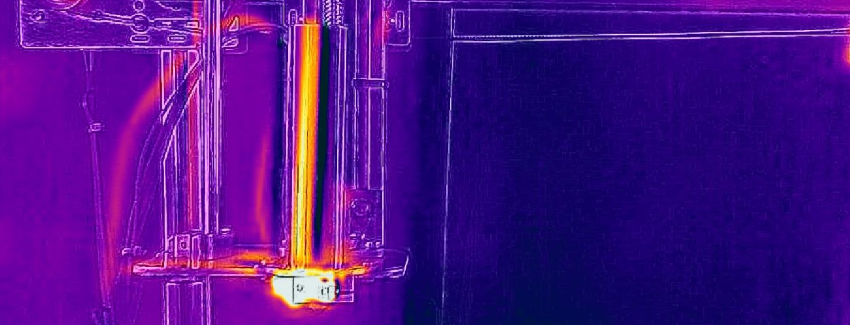
\includegraphics[scale=0.4]{figs/NozTempDistribution.png}
    \caption{Nozzle temperature distribution after 10 minutes of being active (100\% duty cycle)}
    \label{fig:nozdist}
\end{figure}


\begin{figure}[H]
    \centering
    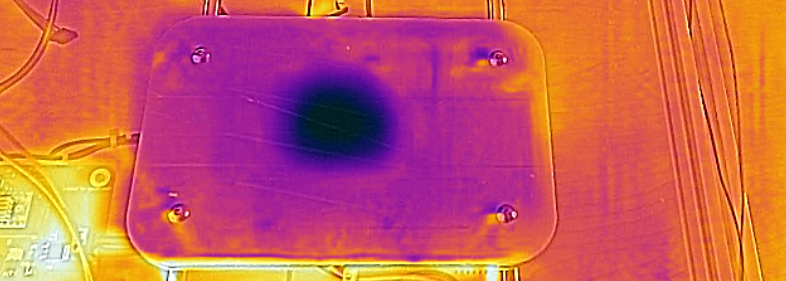
\includegraphics[scale=0.42]{figs/BedTempDist.png}
    \caption{Bed temperature distribution after 10 minutes of being active }
    \label{fig:beddist}
\end{figure}
\chapter{Experimental Design}
The purpose of this chapter is to provide an experimental procedure that allows the custom hydrogel bioprinter to be calibrated for a specific desired hydrogel and to ensure user-safety and reliable operation by providing handling and cleaning instructions. 

The printer's purpose is to serve as a research tool for Stellenbosch University’s Physiology Department, where it will be used both for the characterisation of bioinks and for the fabrication of hydrogel scaffolds to model and simulate cell growth and behaviour in biomedical research. To ensure the hydrogel extrusion system is integrated effectively into this research environment, the chapter establishes protocols for adjusting printing parameters to find the optimal settings for different gels, and details procedures to handle the bioprinter and to clean it after use to maintain hygiene and prevent contamination between experiments which ensures cell viability in cases where the printer is used to print cell-seeded prints. The procedure will be applied to a surrogate gel and documented as an example for use. These guidelines are intended to ensure that the bioprinter can be used consistently, safely, and effectively throughout its utilisation phase.

The calibration procedure involves applying a series of different experiments with the bioprinter and its bioink to optimise its print parameters within different categories of print operations (printing straight, curved, multiple adjacent, and stacked lines). 


\section{Materials and Methods}
\subsection{Materials}
The experimental set-up requires the following equipment and materials:
\begin{itemize}
\item Custom 3D printer with syringe-based extruder
\item Allen Key
\item Bioink solution
\item Laptop (with USB port)
\item Vernier calliper
\item Camera with mount
\end{itemize}

For the surrogate gel (for the example calibration), the following equipment and materials are required:
\begin{itemize}
\item Store-bought Agar Agar powder 
\item Kettle
\item Measurement jug
\item Weight scale
\end{itemize}


The bioprinter comprises of an extruder and a gantry. The extruder uses a lead screw to extrude the gel out of a custom aluminium syringe onto a cooled aluminium bed, and the extrusion force being applied to push the PVC plunger is measured using a load cell and sampled using an STM32F407VGT6 microcontroller. The extruder position relative to the gantry, is varied across 3D space by a gantry that uses belts to adjust the extruder position in the horizontal plain and uses a lead screw to adjust the nozzle height.

The bioprinter’s settings are adjusted using a computer which is used to load the print settings (along with the print movement tasks) onto a microSD card which is inserted into and read by the bioprinter to perform each calibration trial. The laptop is also used to read transmitted USB information from the printer such as extrusion force and the temperature of the nozzle and bed. 

After each print iteration, a photo is taken of the printed strands and its dimensions are analysed in software (ImageJ) to assess the print quality. This experimental set-up is shown below in Figure~\ref{fig:experimentalSetup}:
 \begin{figure}[h]
    \centering
    
\includegraphics[scale=0.7]{figs/ExperimentalSetup.png}
    \caption{Experimental Set-up}
    \label{fig:experimentalSetup}
\end{figure}


\subsection{Equipment Specifications}
The experimental equipment needs to allow a printed line (or multiple lines) of hydrogel to be extruded onto a printing bed where the print line’s width and can be measured at points along the line without distorting the line’s dimensions over the course of the measurement process as this would decrease the reliability of the measurements. The experiment also needs a way to configure the bioprinter’s parameters and receive real time printing feedback.

\subsubsection*{Gel Specifications}
The gel specifications depend on the research needs of the end-user, with each hydrogel type and concentration coming with its own rheological properties and storage and handling protocols.

This experimental procedure, however, was applied to a surrogate gel that is a agar-water mixture. In which store-bought Agar-agar powder is dissolved in water at 2\% w/v. Agar powder was used as it is easy to prepare and gels more rapidly when cooled compared to other store-bought alternatives such as gelatin powder.

\subsubsection*{Bioprinter Specifications}
\begin{itemize}
    \item \textbf{Extruder} – This consists of a syringe with a volume of 20\,ml and a nozzle diameter of 0.4\,mm. The nozzle is capable of reaching a maximum temperature of 95 $^{\circ}$C.
    
    \item \textbf{Gantry} – The gantry is used to position the extruder in 3D space. Two NEMA 17 stepper motors drive belts that control the 2-axis motion in the horizontal plane. A leadscrew (also driven by a NEMA 17) with an 8\,mm lead is used to control the extruder’s vertical position.
    
    \item \textbf{Bed} – The gel is printed on a 110\,mm $\times$ 168\,mm aluminium bed. The bed is capable of reaching a minimum temperature of 4 $^{\circ}$C.
\end{itemize}

\subsubsection*{Software}
\begin{itemize}
    \item \textbf{ImageJ} – This is used to measure the dimensions of the print strands in images of each print iteration.
    \item \textbf{MATLAB} – This is used to graph live data from the printer via USB connection between the laptop and bioprinter. The measurement data from the printing trials are also stored manually and are processed and plotted using MATLAB.
\end{itemize}

\subsection{Methods}

The variables identified, relating to the calibration procedure, are shown below in Table~\ref{tab:variables}:

\begin{longtable}{>{\raggedright\arraybackslash}p{4cm} p{10cm}}
\caption{Experimental Variables} \label{tab:variables}\\
\hline
\textbf{Variable Type} & \textbf{Variables} \\
\hline
Independent Variables & Extrusion rate, printing speed, nozzle height, print line radius, layer count \\
Dependent Variables   & Extrusion force, layer height, layer width, print quality, stack height \\
Controlled Variables  & Gel concentration, print line length nozzle diameter, nozzle temperature, bed temperature \\
Extraneous Variables  & Ambient temperature, vibrations \\
\hline
\end{longtable}

During the analysis of results, the mean layer height and width, stack height, and standard deviation of the layer height and width (in mm) along each of the printed lines are tabulated against the varied printing parameters: extrusion rate (mm/s), printing speed (mm/s), nozzle height (mm), print line radius (mm) and layer count. The two standard deviations serve as separate measures of print quality, where high deviations indicate lower print stability and quality. The total mean height of multiple printed layers will also be measured and calculated along with its standards deviation and compared to its corresponding layer count and layer height increment (mm).

The extrusion force from the load cell, measured via the COM port using MATLAB, is also plotted against time for each of the different extrusion rates. The nozzle diameter affects both the speed and width of the extruded gel, influencing the resulting line width, height, and quality. These dependent variables are also affected by the rheological properties of the gel, which is why the nozzle diameter and gel concentration are kept constant as controlled variables.

Ambient temperature and environmental vibrations, including those from the printer itself, can also influence outcomes. However, these are considered extraneous variables and are not within the scope of control in this experiment.

\subsubsection*{Gel preparation}

The following steps detail how to prepare the agar surrogate gel. It should be noted that these steps must only be followed when the bioprinter is ready to be loaded with the solution (after step 4 of the experimental set-up procedure) and the next print trial is intended to begin within the 5-10 minutes of the completion of the gels preparation to ensure that it does not gel prematurely before its printed.

\begin{enumerate}
    \item Fill the kettle with water and heat water until boiling ($100^{\circ}$C).
    \item From the kettle, pour the boiling water into a clean measurement jug until the bottom of the meniscus reaches the 100\,mL mark on the measuring jug.
    \item Using a digital scale, weigh 2 g of agar-agar powder. 
    \item Slowly mix the powder into the boiling water in the measurement jug. Slowly sprinkle the powder into the water, while stirring with the spoon. After all of of the powder has been sprinkled in the measurement jug, continue stirring until there are no visible clumps remaining in the solution.
\end{enumerate}

\subsubsection*{Experimental Set-up Procedure}
Before the calibration can be conducted, the a set-up procedure must first be conducted. Due to the bioprinter's ability to heat its nozzle and syringe, it is best that this step is repeated before every printing trial (loaded onto the microSD card), to ensure the system operator does not come into direct contact with the potentially high syringe temperatures.
\begin{enumerate}
    \item Using the laptop, load the print settings and print tasks (according to the needs of the specific experimental trial that is being conducted) onto the microSD card.
    \item Insert the card into the bioprinter circuit board's microSD port and connect the laptop to the printer's PCB via USB cable. A blue LED on the PCB will light up once the USB connection is established.
    \item Ensure the MATLAB graphing software has been opened and is running.
    \item Using the Allen Key, unbolt the syringe from the extruder assembly and unscrew the syringe hot-end from the metal syringe tip.
    \item Check and ensure syringe is clean and press the plunger until it is fully depressed to the bottom of the syringe tube.
    \item Once the gel solution is ready for use (see the gel preparation procedure or the handling/preparation steps of the desired bioink), submerge the tip of the syringe into the substance and pull the plunger until it reaches the end of the syringe or a sufficient volume of the solution is extracted.
    \item Once the printer fluid has been loaded, wipe the syringe sections that were submerged during extraction, with a cloth.
    \item Screw the hot-end assembly back on to the threaded syringe tip and mount the flanged syringe back onto the extruder platform using the bolts and Allen Key (make sure at least two bolts are fastened along the PCD (flange mounting holes).
    \item Plug in the 3D printer's 3 prong plug into the wall socket to provide power to the system. The system will initialize according to the print settings on the microSD card and once it is homed and the bed and nozzle have reached their set temperature, the bioprinter will begin its print trial. 
    \item Do not touch the printer during operation and keep the area around moving parts and nip points clear of loose items.
    \item Monitor the bed and syringe temperature through MATLAB as well as the extrusion force to ensure safe printer operation.
    \item Once the print trial is done, use a camera to take a photo of the results.
    \item Analyse the results in ImageJ.
    \item Perform clean-up procedure.
\end{enumerate}
\subsubsection*{Straight Line Test Procedure}

Once the setup is complete, the following test procedure is performed:

\begin{enumerate}
    \item Use STM32CubeIDE to vary the extrusion rate (mm/s), printing speed (mm/s), and nozzle offset (mm).
    \item Begin the extrusion process to deposit a 10\,mm long GelMA line onto the bed. Monitor the print using Termite.
    \item Use MATLAB to acquire and process the time-based extrusion force data for each extrusion rate.
    \item After printing, if no UV shielding is present, evacuate the room while the UV light cures the print for 5 minutes.
    \item Re-enter the room and measure the printed line’s width and height at 10 equidistant points (1\,mm apart) using a digital caliper.
    \item Record the mean and standard deviation of the 10 measurements for both width and height. These serve as metrics for print stability and quality.
    \item Repeat each test condition three times. Compute 95\% confidence intervals for each of the four measured variables (mean and standard deviation of width and height) to quantify measurement uncertainty and evaluate repeatability.
\end{enumerate}

A proposed test matrix is shown in Table~\ref{tab:testmatrix}, which outlines the combination of printing parameters for each trial in the experiment.

\begin{longtable}{ccc}
\caption{Proposed Test Matrix for Each Experiment} \label{tab:testmatrix} \\
\hline
\textbf{Test No.} & \textbf{Printing Speed (mm/s)} & \textbf{Extrusion Speed (mm/s)} \\
\hline
1  & 1 & 0.025 \\
2  & 1 & 0.050 \\
3  & 1 & 0.075 \\
4  & 1 & 0.100 \\
5  & 2 & 0.025 \\
6  & 2 & 0.050 \\
7  & 2 & 0.075 \\
8  & 2 & 0.100 \\
9  & 3 & 0.025 \\
10 & 3 & 0.050 \\
11 & 3 & 0.075 \\
12 & 3 & 0.100 \\
13 & 4 & 0.025 \\
14 & 4 & 0.050 \\
15 & 4 & 0.075 \\
16 & 4 & 0.100 \\
\hline
\end{longtable}
These tests are split up into two experiments, two compare the variation of nozzle offset. In experiment A, the nozzle offset is set to 2mm and in experiment B, it is set to 4mm.

\subsubsection*{Curved Line Test Procedure}

\subsubsection*{Layer Stacking Test Procedure}

\subsubsection*{Cleaning Procedure}

\section{Discussion of Results and Conclusion}
\chapter{Conclusions}

With the extruder and PCB design completed. The next steps are to start ordering parts and begin the assembly of these systems and complete the last design changes to the gantry with its bed design.



\appendix%------------------------------------------------------------
\chapter{Calculations}

\section{Syringe Calculations}

\textbf{Given:}
\begin{align*}
\text{Inner diameter of barrel (ID}_1\text{)} &= \SI{20}{\milli\meter} \\
\text{Length of barrel (L}_1\text{)} &= \SI{80}{\milli\meter} \\
\text{Inner diameter of nozzle (ID}_2\text{)} &= \SI{0.2}{\milli\meter} \\
\text{Length of nozzle (L}_2\text{)} &= \SI{20}{\milli\meter}
\end{align*}

\noindent\textbf{Cross-sectional areas:}
\begin{align*}
A_1 &= \pi \left(10 \times 10^{-3}\right)^2 \approx 314 \times 10^{-6} \, \si{\meter\squared} \\
A_2 &= \pi \left(0.1 \times 10^{-3}\right)^2 \approx 31.4 \times 10^{-9} \, \si{\meter\squared}
\end{align*}

\noindent\textbf{Max extrusion speed at nozzle:}
\[
v = \SI{5}{\milli\meter\per\second} = 5 \times 10^{-3} \, \si{\meter\per\second}
\]

\noindent\textbf{Volumetric flow rate:}
\[
Q = v \cdot A_2 = (5 \times 10^{-3}) \cdot (31.4 \times 10^{-9}) = 1.57 \times 10^{-10} \, \si{\meter\cubed\per\second}
\]

\noindent\textbf{Assumed viscosity:} 
\[
\mu = \SI{1}{\pascal\second}
\]

\noindent\textbf{Poiseuille's Law:}
\[
\Delta P = \frac{8 \mu L Q}{\pi r^4}
\]

\noindent\textbf{Total pressure required:}
\begin{align*}
P_{\text{atm}} &= \SI{101325}{\pascal} \\
P_{\text{Plunger}} &= \Delta P_{\text{ID}_1} + \Delta P_{\text{ID}_2} + P_{\text{atm}} \\
&= \frac{8 \cdot 1 \cdot 0.08 \cdot (1.57 \times 10^{-10})}{\pi (0.01)^4}
+ \frac{8 \cdot 1 \cdot 0.02 \cdot (1.57 \times 10^{-10})}{\pi (0.0001)^4}
+ 101325 \\
&= \SI{181325}{\pascal} = \boxed{\SI{181.3}{\kilo\pascal}}
\end{align*}

\noindent\textbf{Required force:}
\[
F = P \cdot A_1 = (181\,325)\cdot(314 \times 10^{-6}) = \SI{56.94}{\newton}
\]

\noindent\textbf{Design force (with safety factor):}
\[
F_{\text{SF}} = \SI{300}{\newton}
\]

\noindent\textbf{Required torque for lead screw to produce axial force:}
\begin{itemize}
  \item Axial force: \( F = 300\,\text{N} \)
  \item Coefficient of friction: \( \mu = 0.2 \)
  \item Lead: \( l = 8\,\text{mm} = 0.008\,\text{m} \)
  \item Pitch: \(p=2\,\text{mm}\)
  \item Diameter: \(d=8\,\text{mm}\)
  \item Mean diameter: \( d_m = d-\frac{p}{2} = 7\,\text{mm}\)
\end{itemize}


\begin{align*}
T &= \frac{F d_m}{2} \cdot \left( \frac{l + \pi \mu d_m}{\pi d_m - \mu l} \right) \\
  &= \frac{(300)(0.007)}{2} \cdot \left( \frac{0.008 + \pi(0.2)(0.007)}{\pi(0.007) - (0.2)(0.008)} \right) \\
  &= 0.638\,\text{N}\cdot\text{m}
\end{align*}


\section{Z Axis Lead Screw Calculations}

\textbf{Assumptions:}
\begin{itemize}
  \item Load mass: \( m = 1.86\,\,\text{kg} \)
\end{itemize}

\noindent\textbf{Required lifting force:}  

\( F = mg = 1.86 \cdot 9.81 = 18.25\,\text{N} \)

\noindent\textbf{Required torque for lead screw to produce axial force:}
\begin{align*}
T &= \frac{F d_m}{2} \cdot \left( \frac{l + \pi \mu d_m}{\pi d_m - \mu l} \right) \\
  &= \frac{18.25 \cdot 0.007}{2} \cdot \left( \frac{0.008 + \pi \cdot 0.2 \cdot 0.007}{\pi \cdot 0.007 - 0.2 \cdot 0.008} \right) \\
  &= 0.0388\,\text{N}\cdot\text{m}
\end{align*}


\section{X and Y Axis Belt and Pulley Calculations}

\textbf{Assumptions:}
\begin{itemize}
  \item Mass: \( m_x = 0.39\,\text{kg} \), \( m_y = 1.02\,\text{kg}\)
  \item Desired acceleration: \( a = 5\,\text{m/s}^2 \)
  \item Coefficient of friction: \( \mu = 0.2 \)
\end{itemize}

\noindent\textbf{Required belt force along the X axis:}
\[ F_{\text{x,inertia}} = m_x \cdot a = 0.39 \cdot 5 = 1.95\,\text{N} \]
\[ F_{\text{x,friction}} = \mu \cdot m_x \cdot g = 0.2 \cdot 0.39\cdot 9.81 = 0.77\,\text{N} \]
\[
 F_{\text{x,total}} = F_{\text{x,inertia}} + F_{\text{x,friction}} = 1.95 + 0.77 = \boxed{2.72\,\text{N}}
\]

\noindent\textbf{Required pulley torque to produce belt force in the X direction:}

\noindent A GT2 20T pulley has a diameter of:
\[
  d_p = \frac{t \cdot N}{\pi} = \frac{2 \cdot 20}{\pi} \approx 12.73\,\text{mm} = 0.01273\,\text{m}
  \]

Therefore, the required torque is:

\[
T = F \cdot \frac{d_p}{2} = 2.72 \cdot \frac{0.01273}{2} = \boxed{0.0173\,\text{Nm}}
\]


\noindent\textbf{Required belt force along the Y axis:}
\[ F_{\text{y,inertia}} = m_y \cdot a = 1.02 \cdot 5 = 5.1\,\text{N} \]
\[ F_{\text{y,friction}} = \mu \cdot m_y \cdot g = 0.2 \cdot 1.02 \cdot 9.81 = 2.00\,\text{N} \]
\[
 F_{\text{y,total}} = F_{\text{y,inertia}} + F_{\text{y,friction}} = 5.1 + 2.00 = \boxed{7.1\,\text{N}}
\]


\noindent\textbf{Required pulley torque to produce belt force in the Y direction:}

\noindent A GT2 36T pulley has a diameter of:
\[
  d_p = \frac{t \cdot N}{\pi} = \frac{2 \cdot 36}{\pi} \approx 22.92\,\text{mm} = 0.02292\,\text{m}
\]

Therefore, the required torque is:

\[
T = F \cdot \frac{d_p}{2} = 7.1 \cdot \frac{0.02292}{2} = \boxed{0.08137\,\text{Nm}}
\]
\chapter{Mechanical Drawings}

\begin{center}
  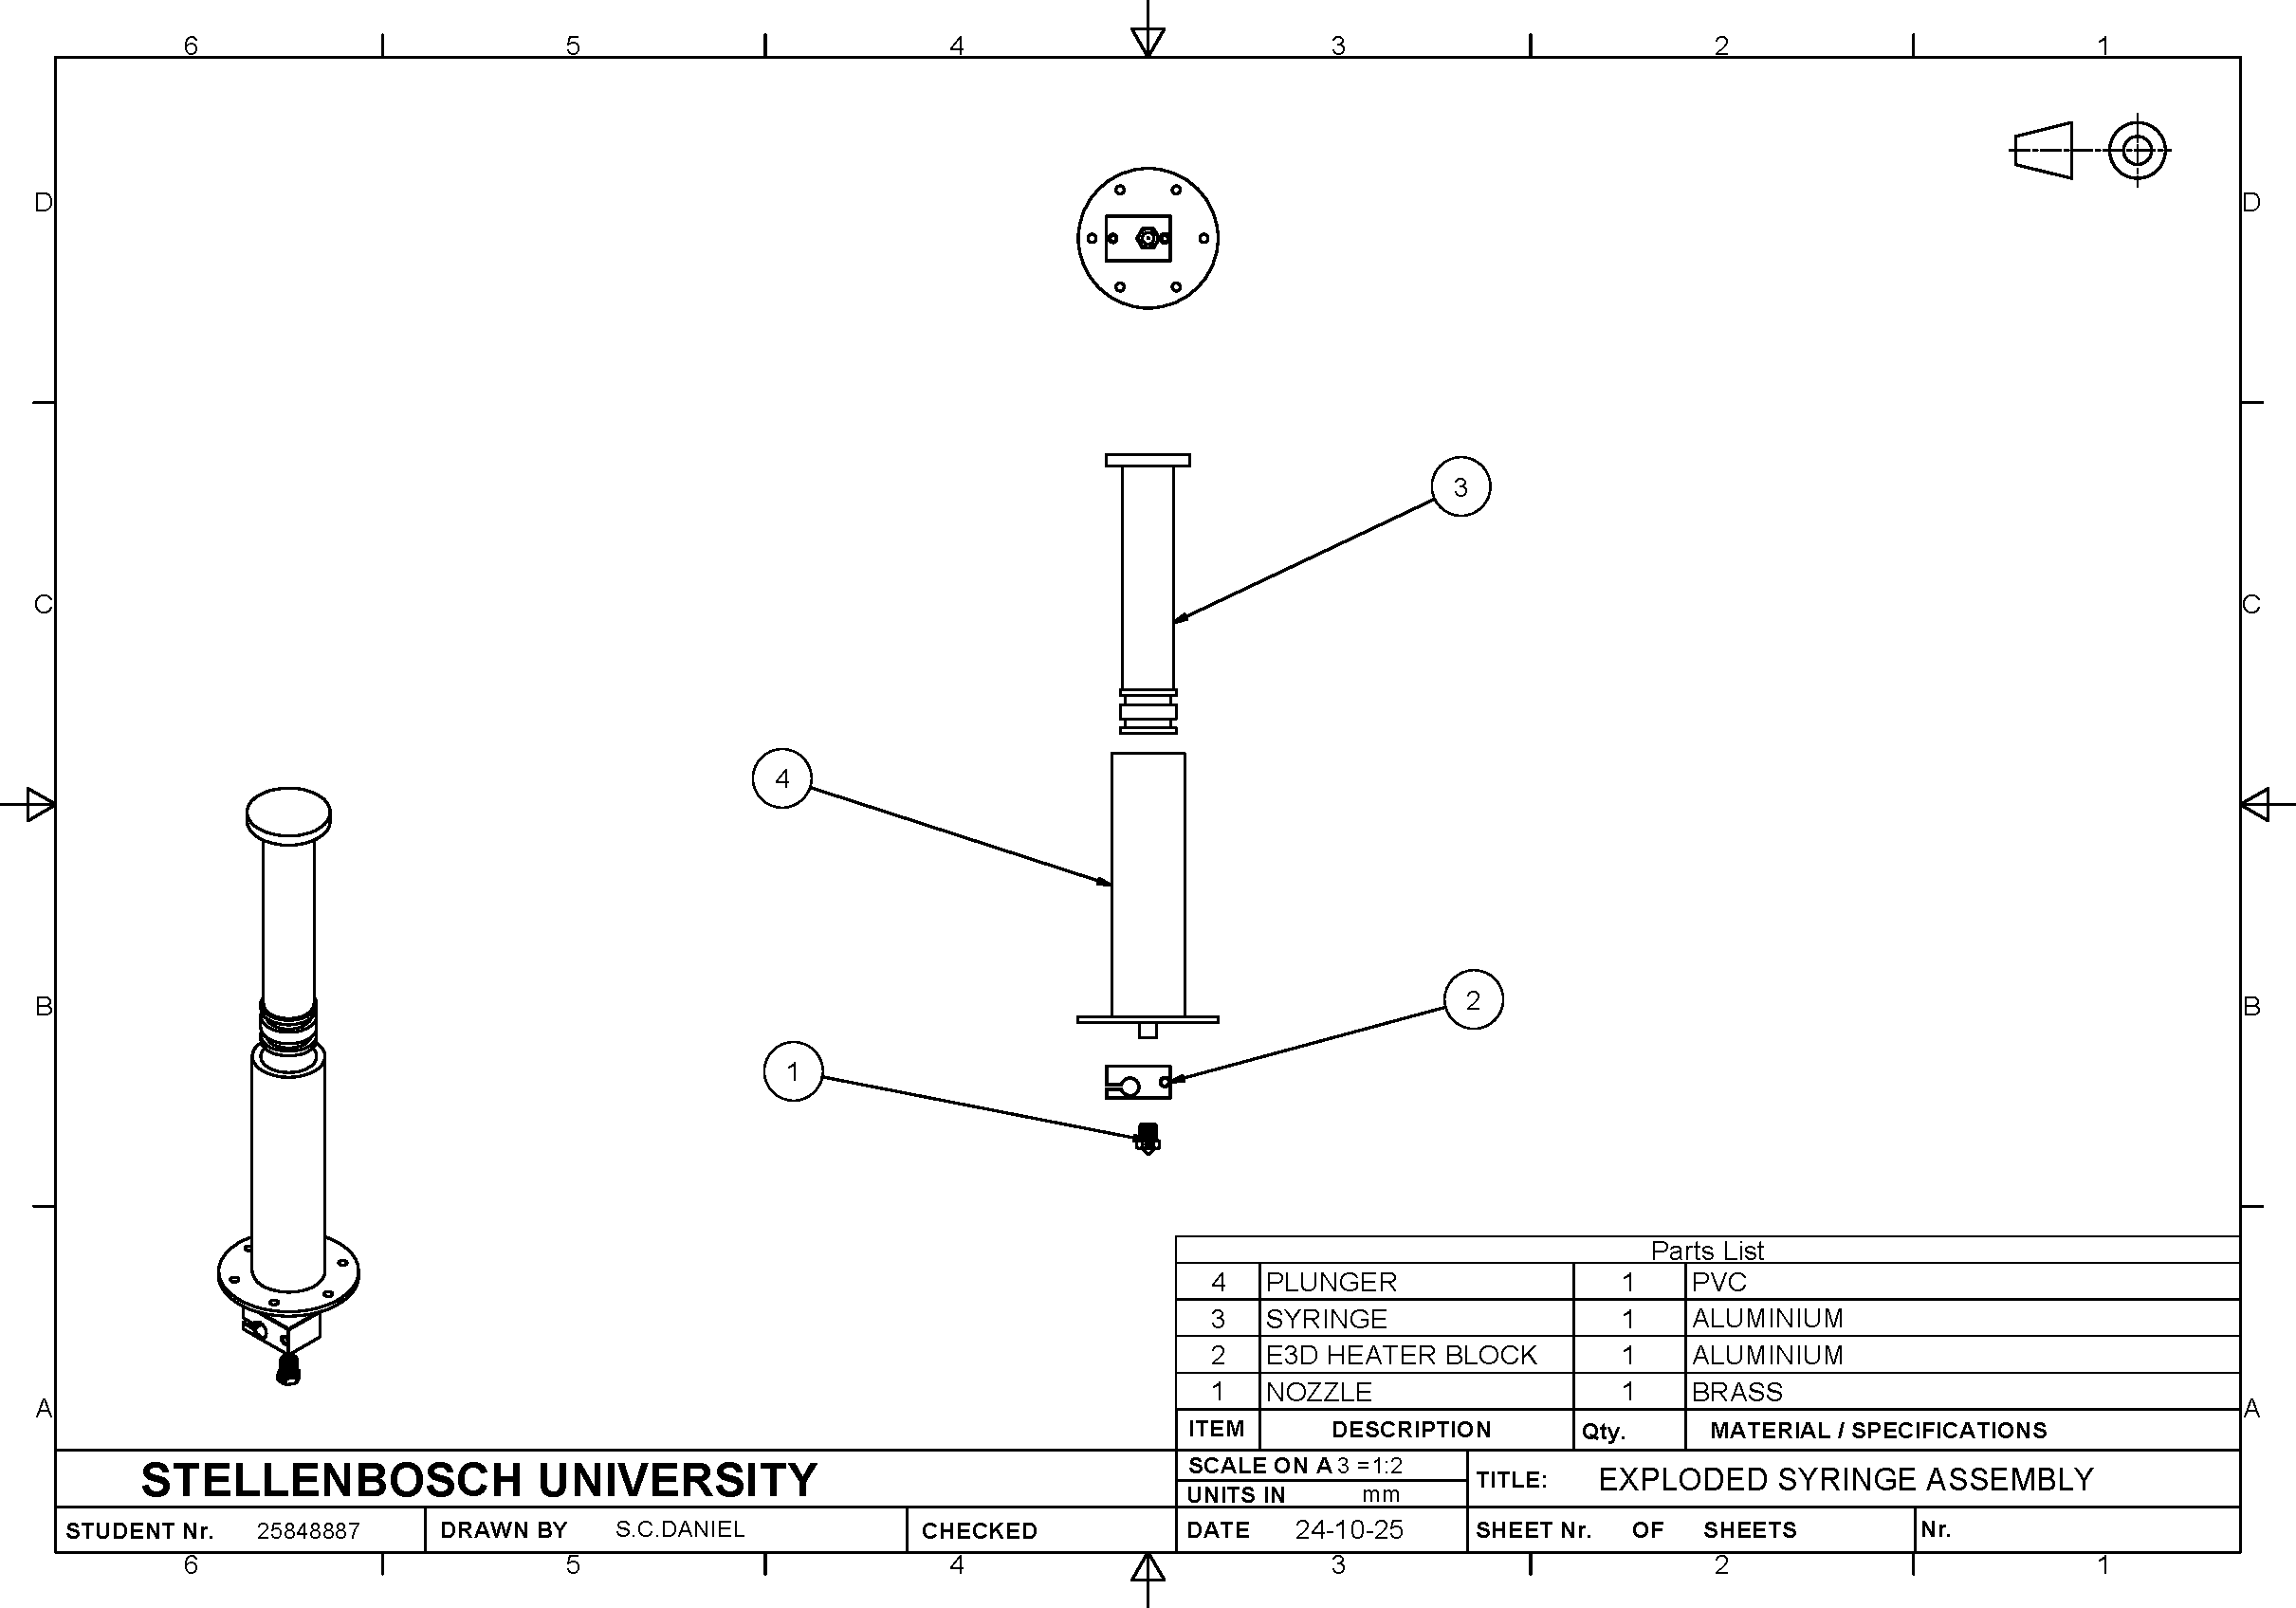
\includegraphics[angle=90, width=0.45\textheight]{chaps-append/20) Syringe Assembly - Exploded view.pdf}
  \captionof{figure}{Mechanical drawing of the exploded syringe assembly.}
  \label{fig:explode}
\end{center}

\chapter{Embedded Hardware}

\noindent This appendix shows the complete embedded system hardware design, including the 3D model, copper layer layouts, and schematic pages for the hydrogel 3D printer control circuit.

\section{PCB Layout}
\begin{center}
  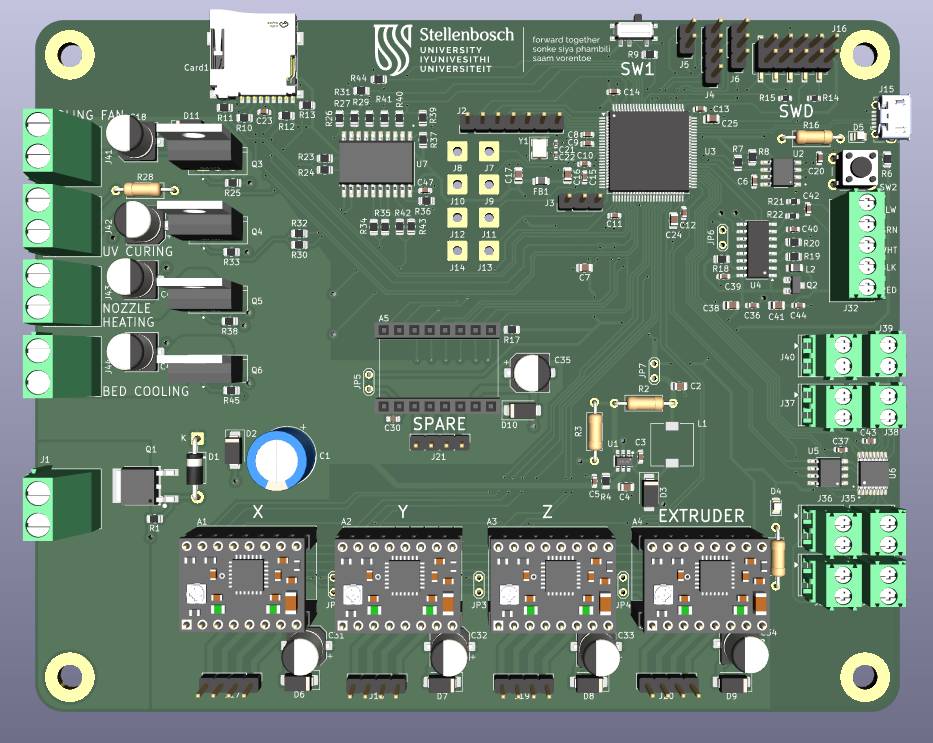
\includegraphics[width=0.62\textheight]{chaps-append/PCB_3D_view.png}
  \captionof{figure}{3D model of the assembled PCB illustrating overall component layout}
  \label{fig:pcb_3d_view}

  \vspace{1em}
  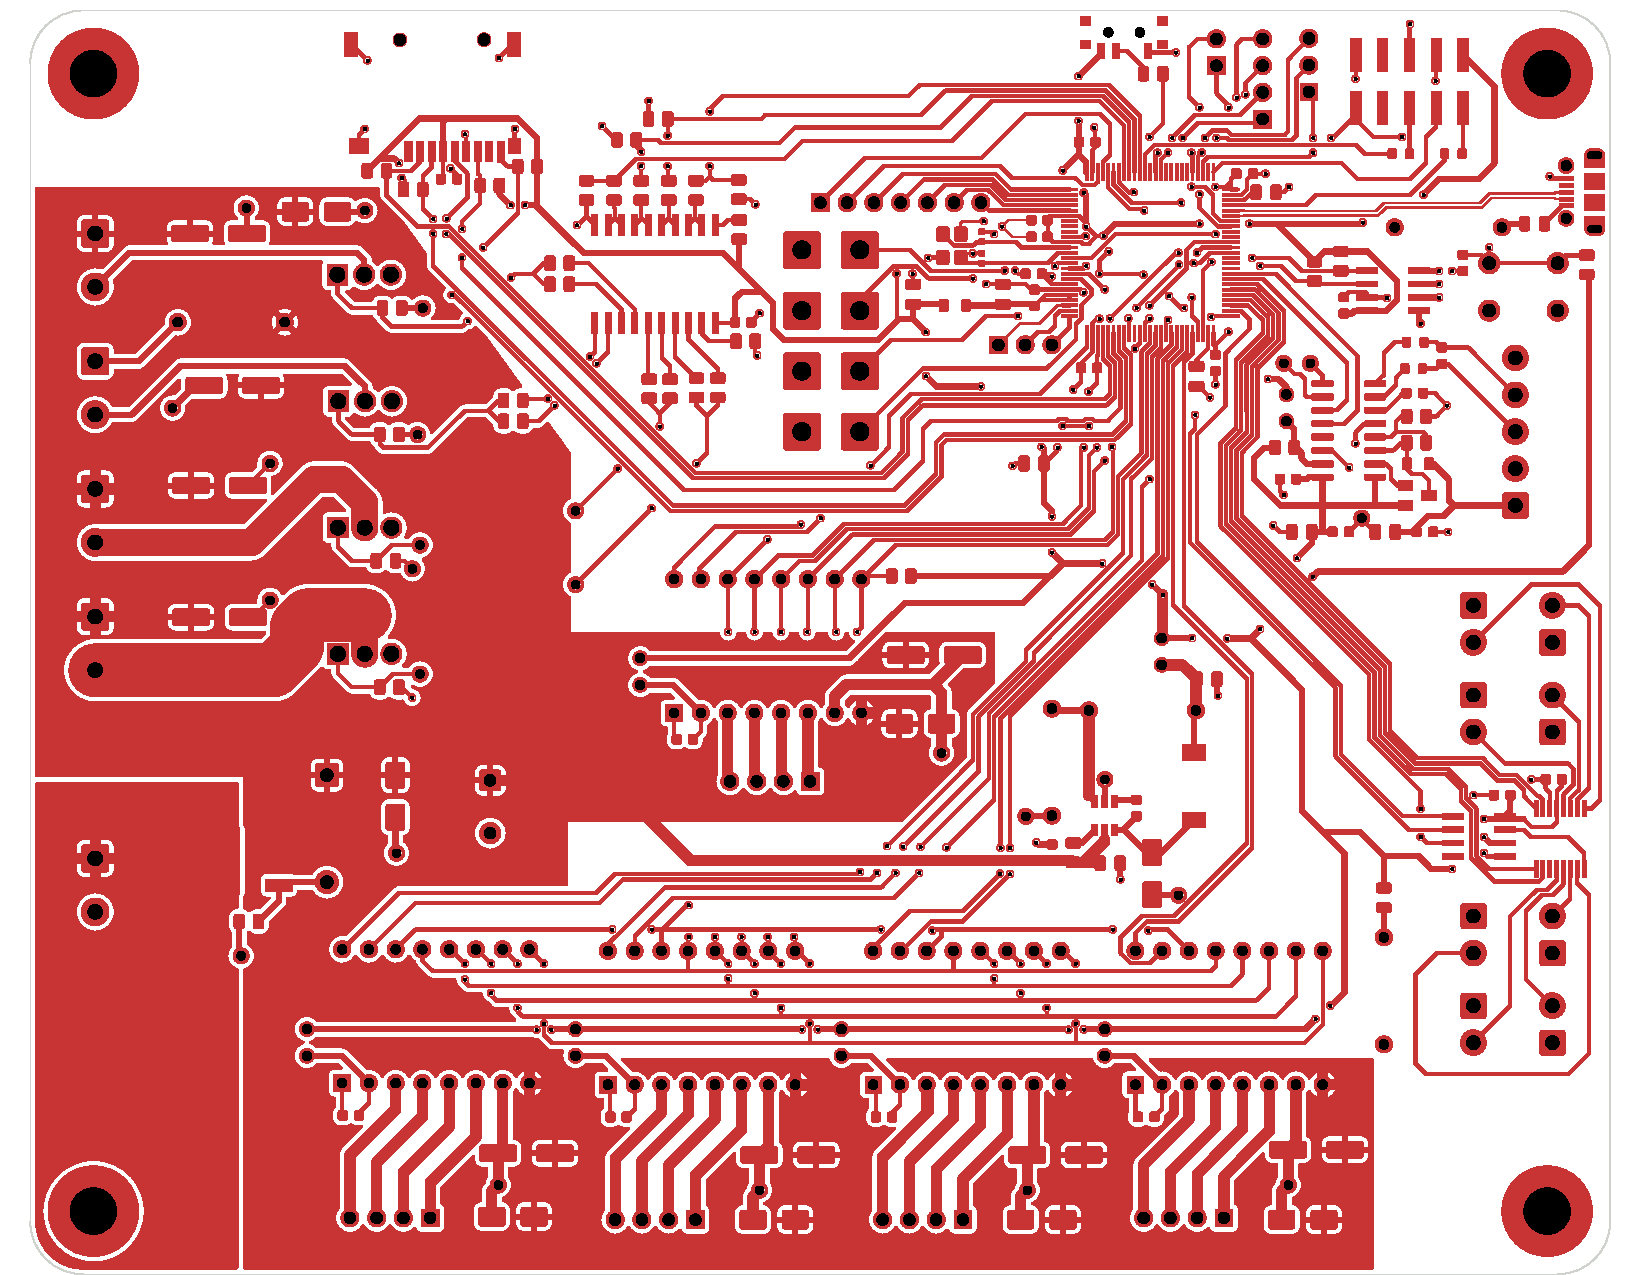
\includegraphics[width=0.56\textheight]{chaps-append/PCB_top_layer.pdf}
  \captionof{figure}{Top layer layout showing signal routing and power traces.}
  \label{fig:pcb_top_layer}

  \vspace{1em}
  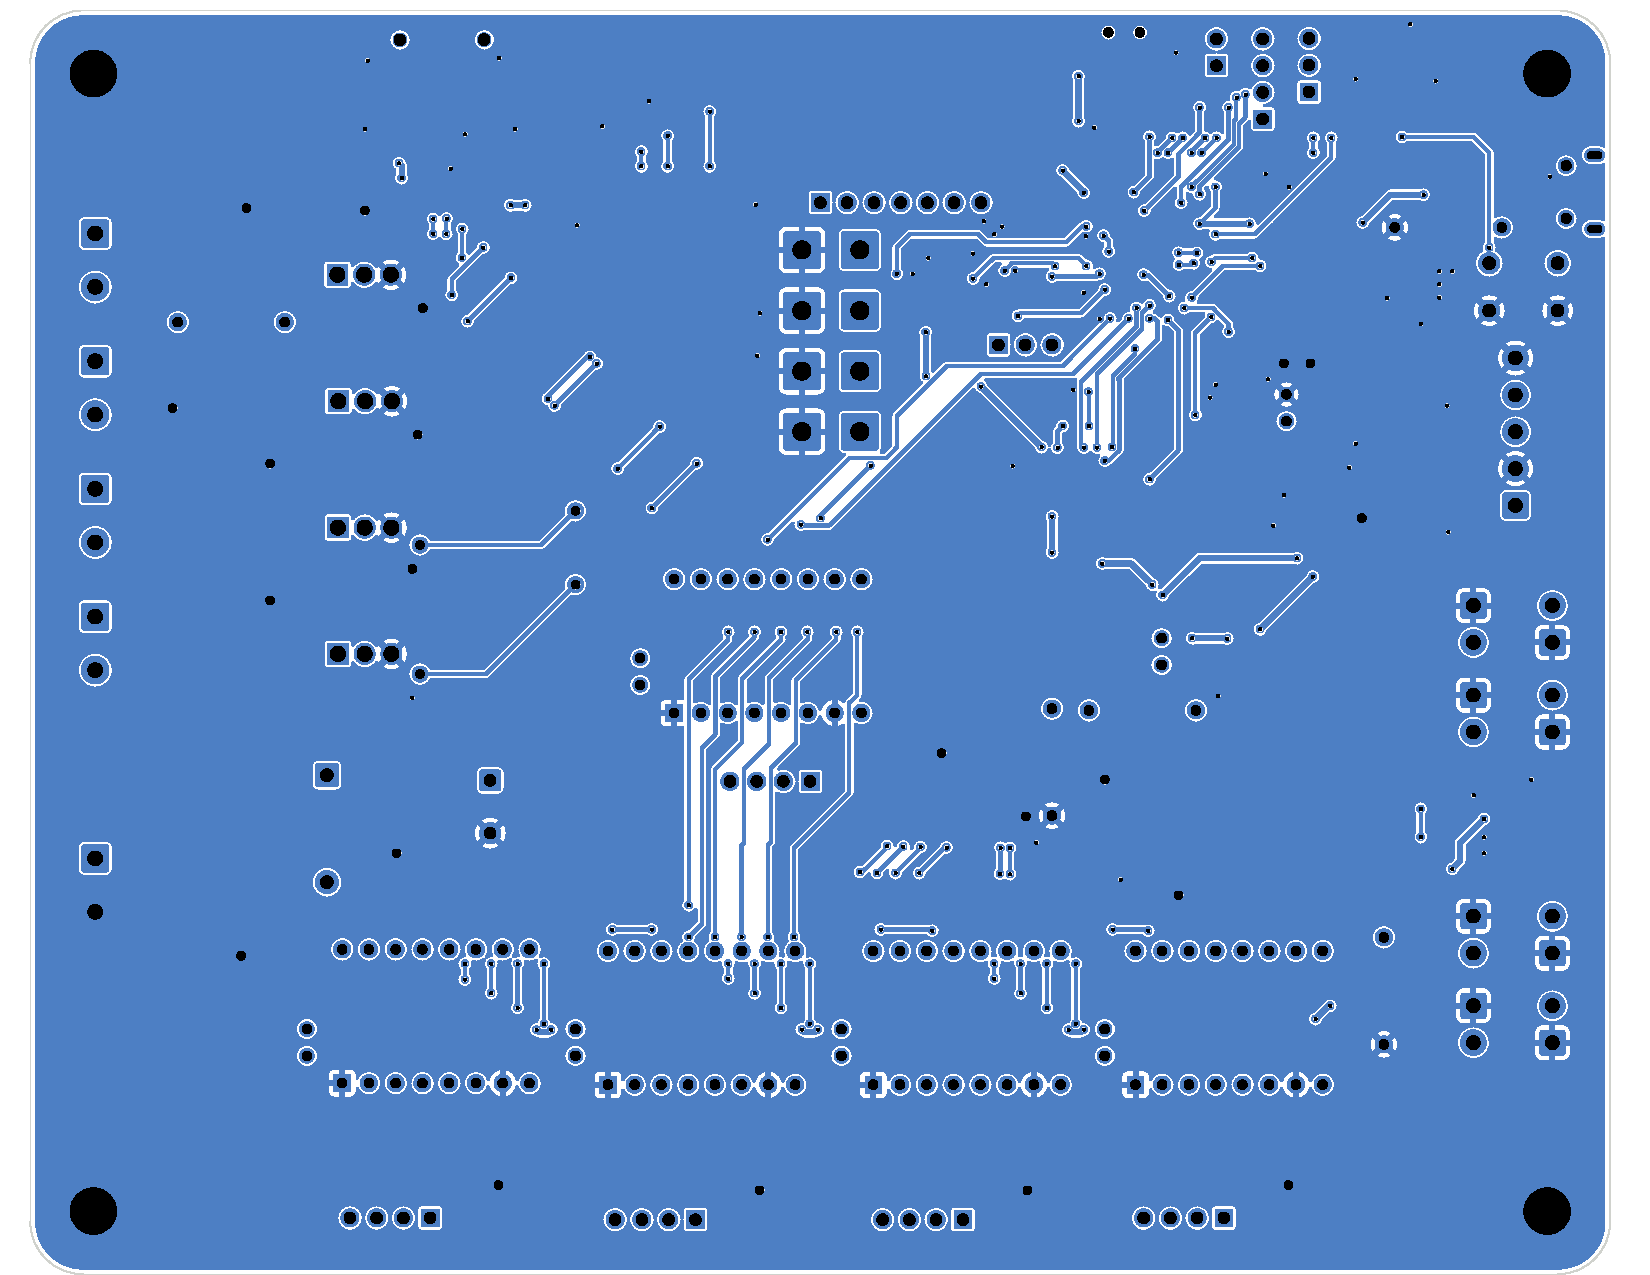
\includegraphics[width=0.56\textheight]{chaps-append/PCB_bottom_layer.pdf}
  \captionof{figure}{Bottom layer layout showing ground planes, vias, and routing.}
  \label{fig:pcb_bottom_layer}
\end{center}

\section{Circuit Schematics}
\begin{center}
  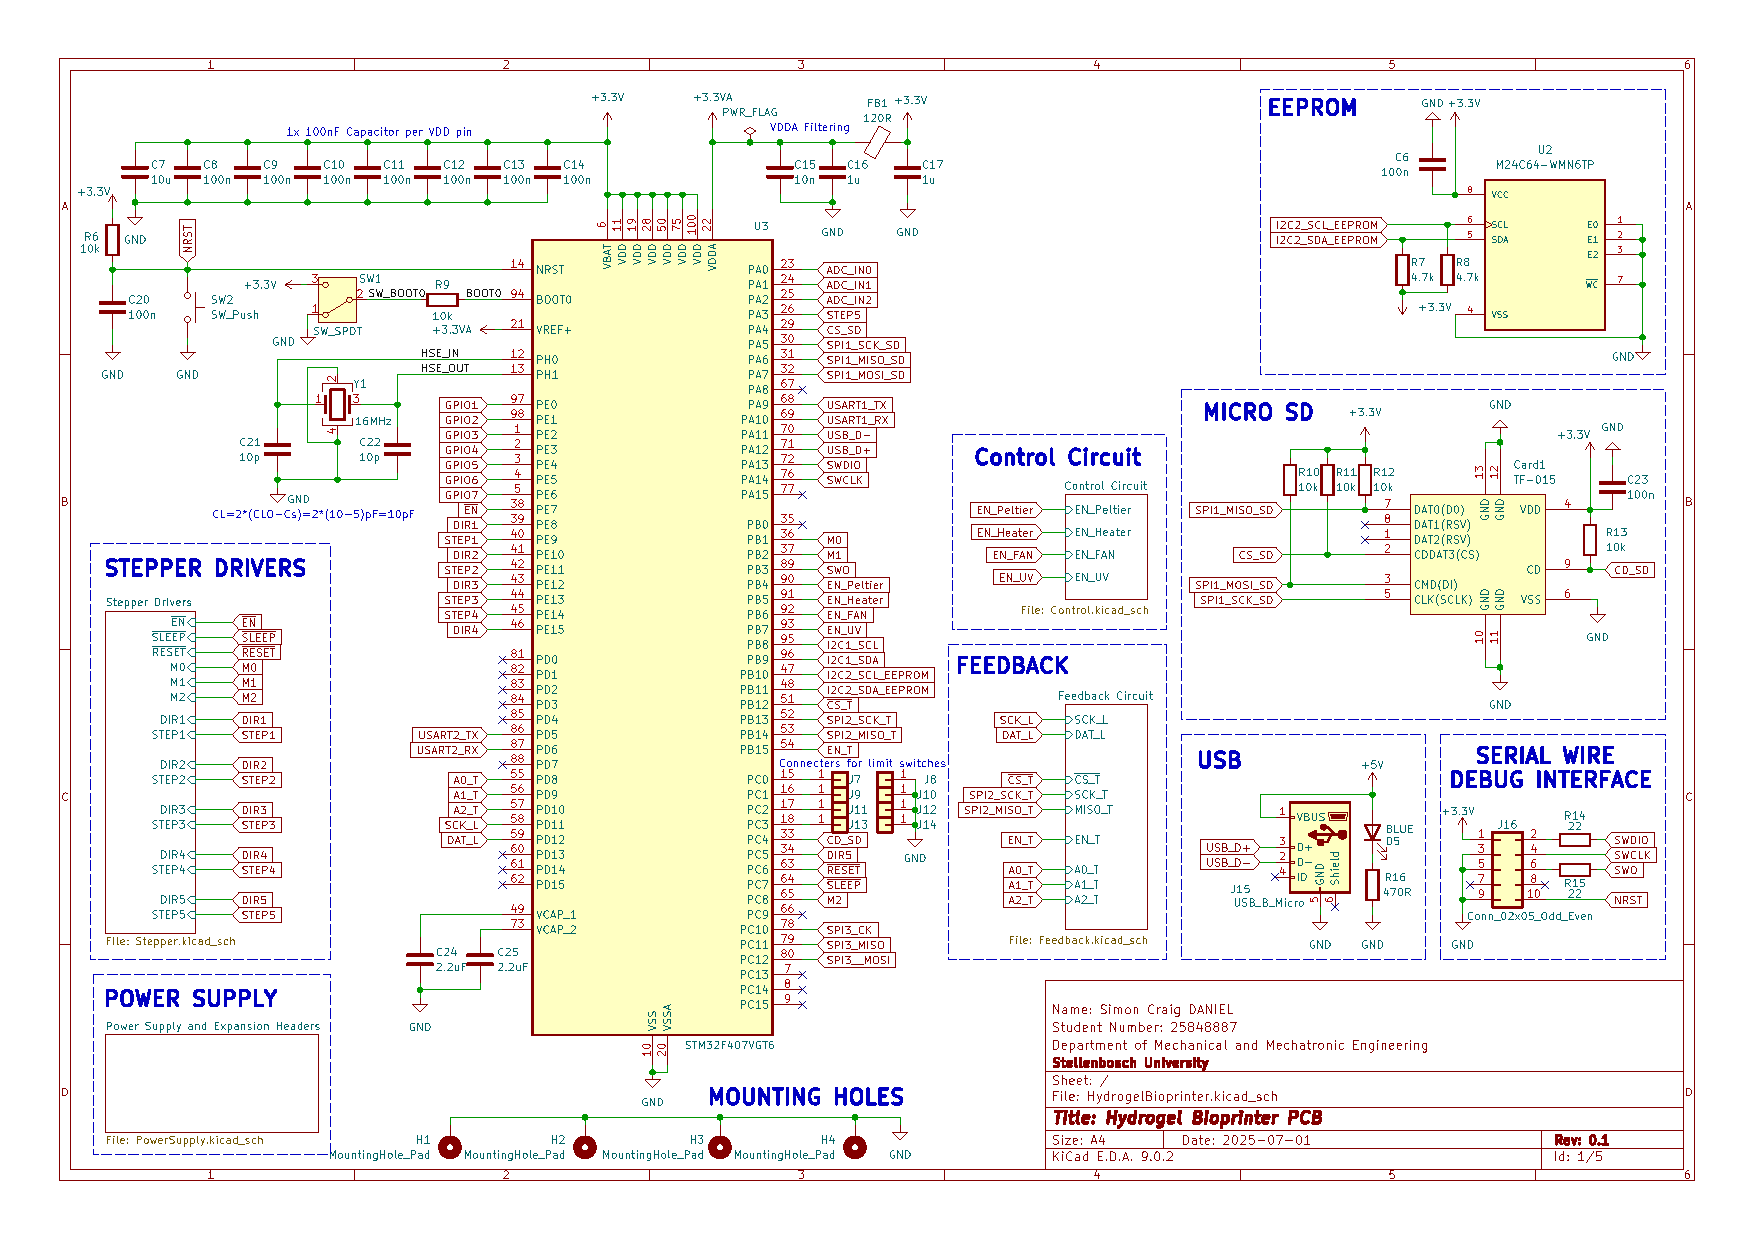
\includegraphics[angle=90, width=0.64\textheight]{chaps-append/PCBSchematic_Page1.pdf}
  \captionof{figure}{Schematic overview of the bioprinter control board.}
  \label{fig:pcb_overview}

  \vspace{1em}
  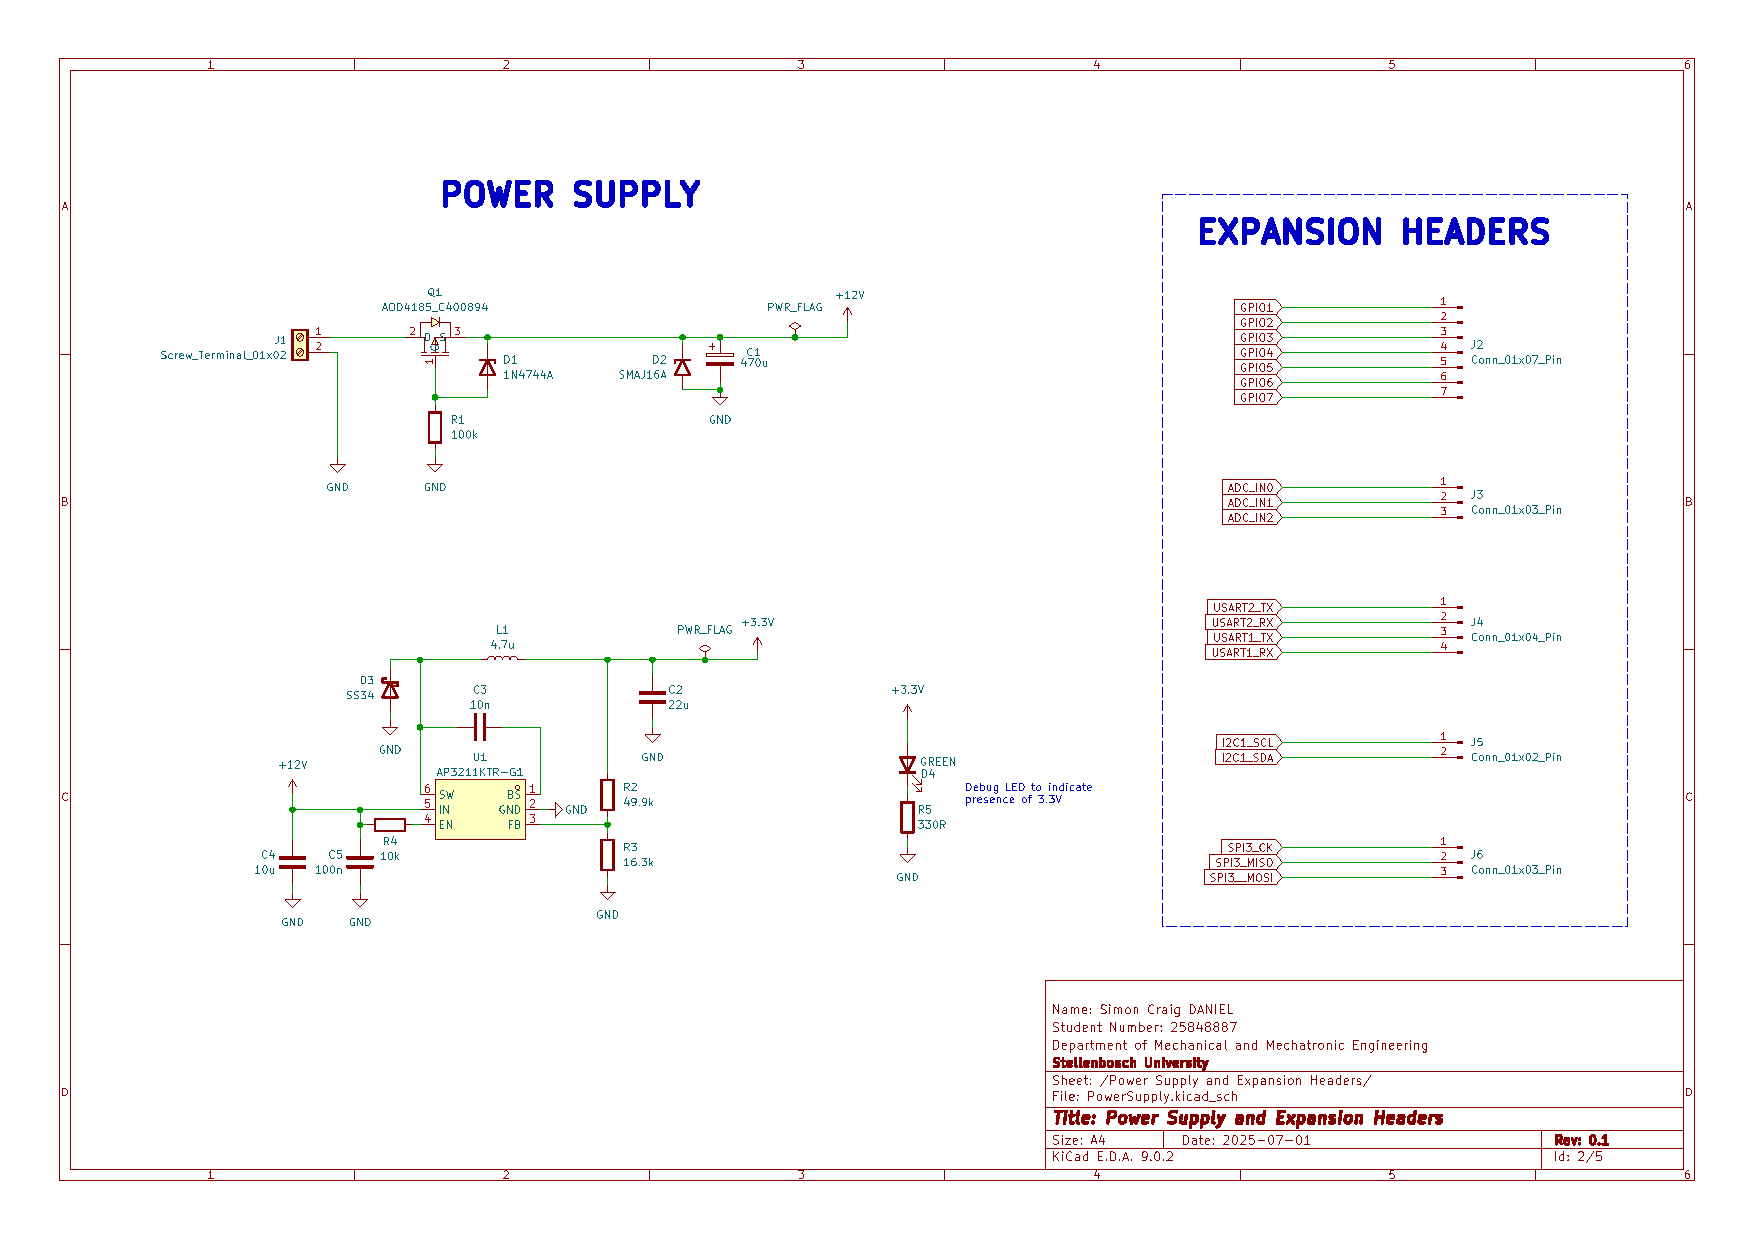
\includegraphics[angle=90, width=0.64\textheight]{chaps-append/PCBSchematic_Page2.pdf}
  \captionof{figure}{Bioprinter power supply system schematic.}
  \label{fig:pcb_power}

  \vspace{1em}
  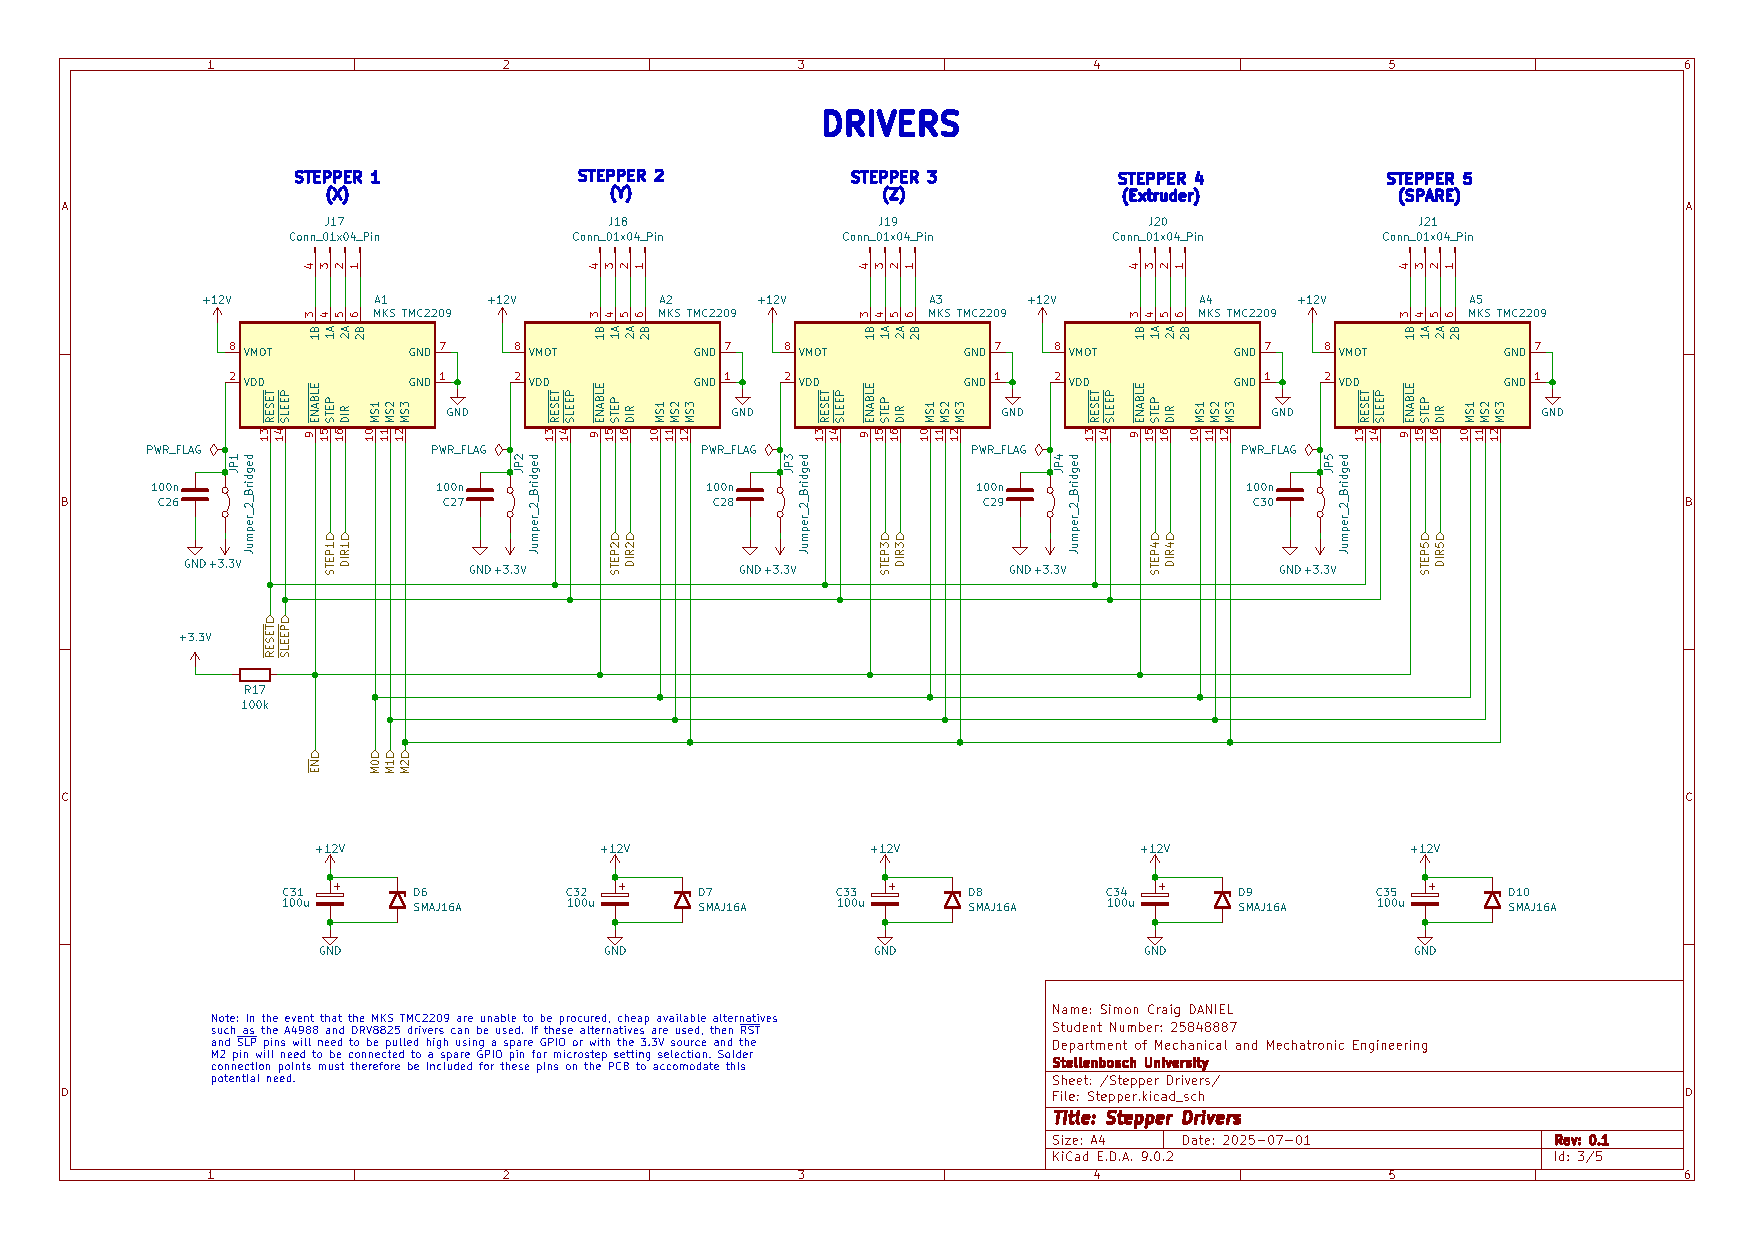
\includegraphics[angle=90, width=0.64\textheight]{chaps-append/PCBSchematic_Page3.pdf}
  \captionof{figure}{Bioprinter stepper driver system schematic.}
  \label{fig:pcb_steppers}

  \vspace{1em}
  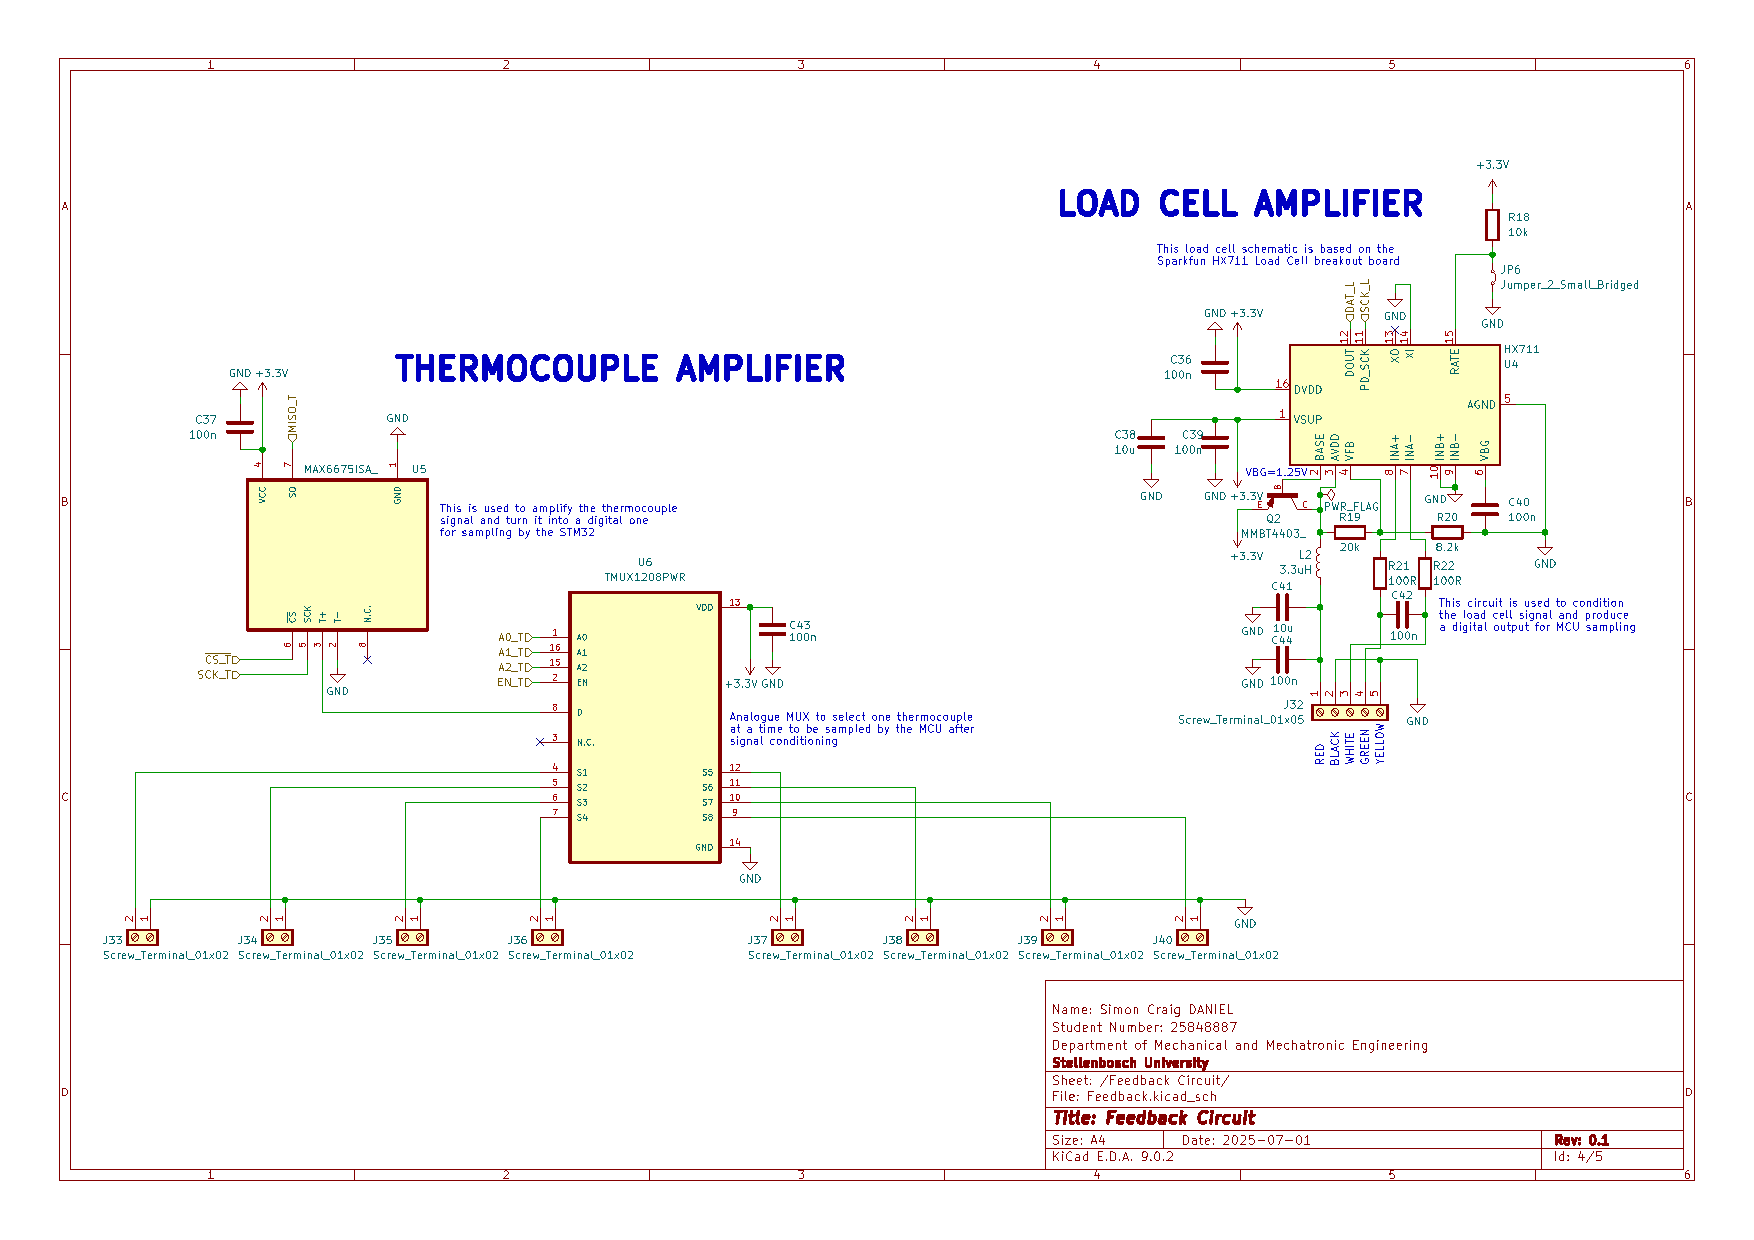
\includegraphics[angle=90, width=0.64\textheight]{chaps-append/PCBSchematic_Page4.pdf}
  \captionof{figure}{Bioprinter sensor system schematic.}
  \label{fig:pcb_sensors}

  \vspace{1em}
  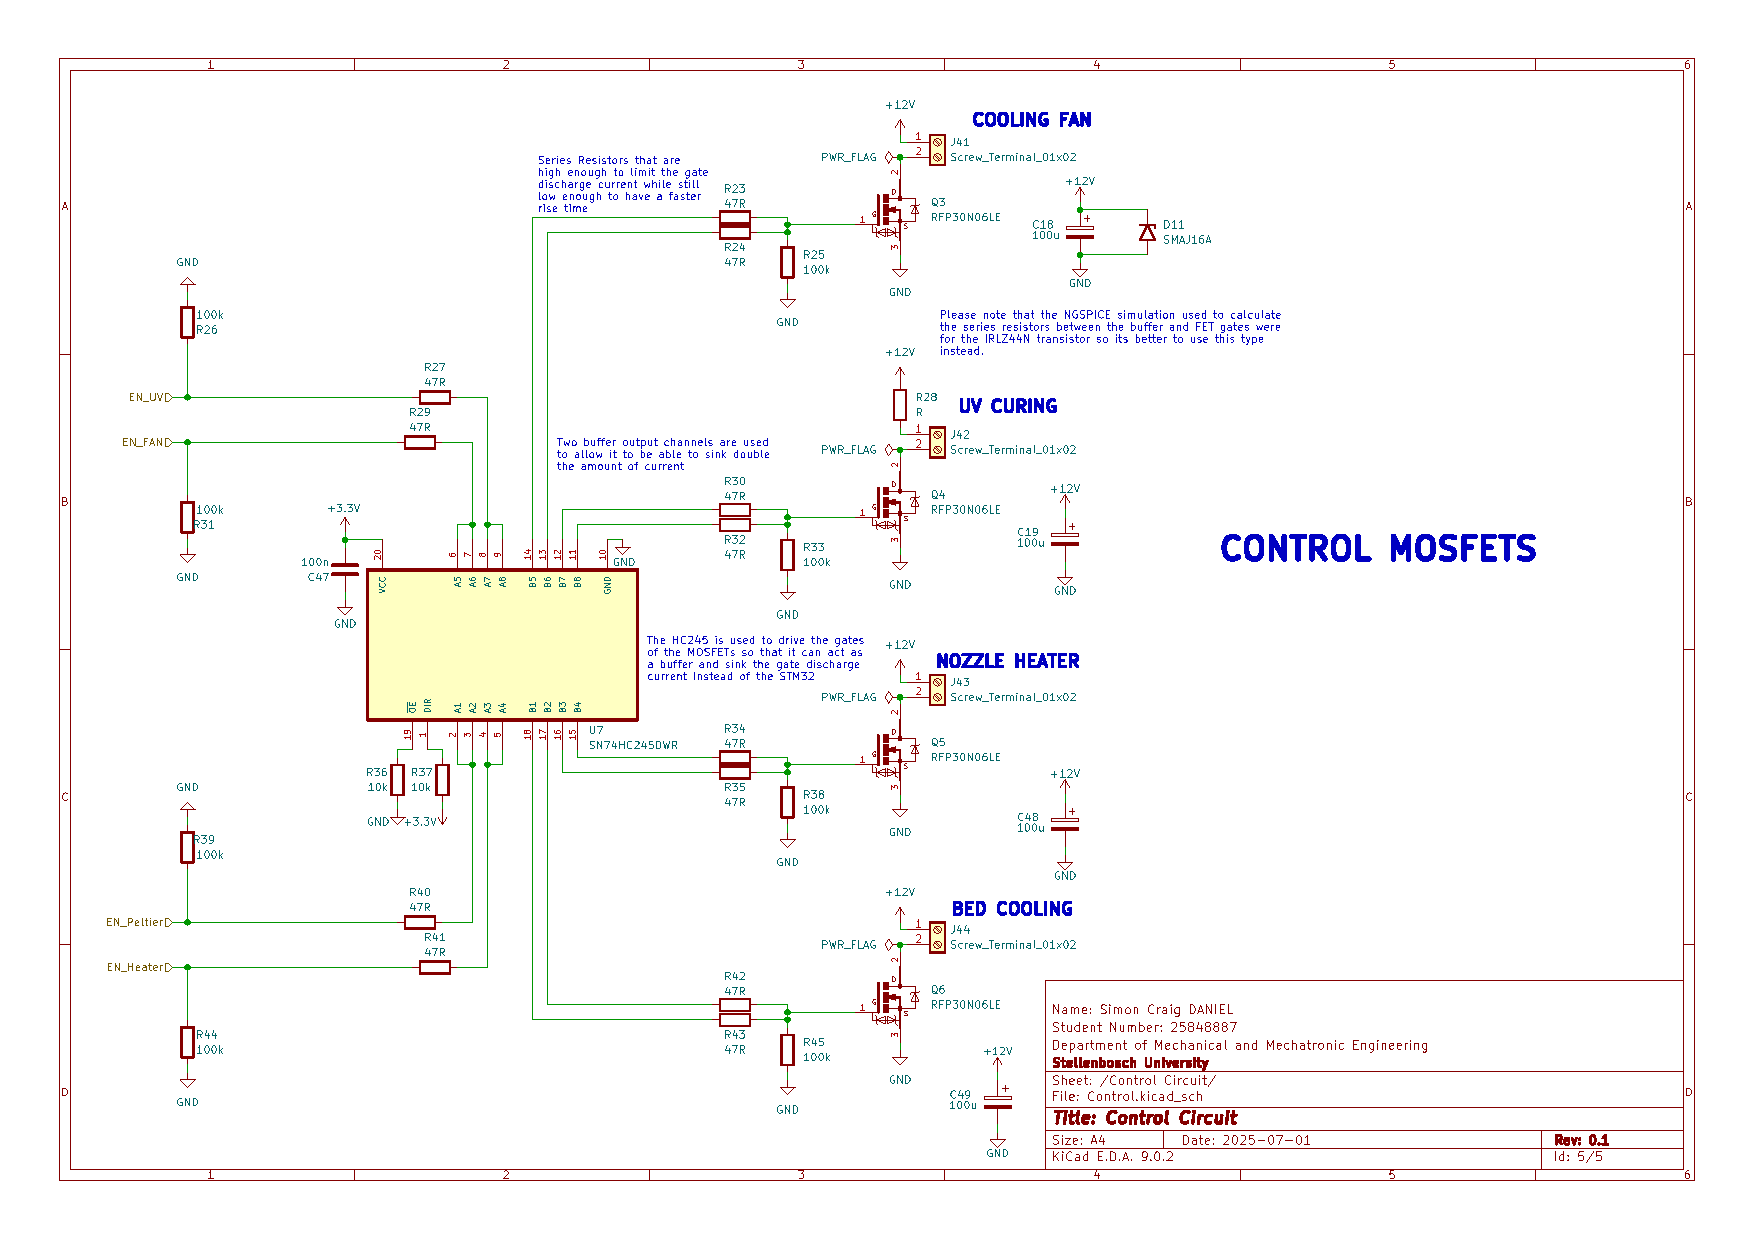
\includegraphics[angle=90, width=0.64\textheight]{chaps-append/PCBSchematic_Page5.pdf}
  \captionof{figure}{Bioprinter control circuit schematic.}
  \label{fig:pcb_control}
\end{center}

\chapter{Experimental Calibration}
\section{Calibration Test Matrices}
{\small
\begin{longtable}{ccc}
\caption{Proposed Test Matrix for Optimal Nozzle height} \label{tab:heightmatrix} \\
\hline
\textbf{Test No.} & \textbf{Nozzle Height (mm)} \\
\hline
\endhead
\hline
1 & 0.2 \\
2 & 0.4 \\
3 & 0.6 \\
4 & 0.8 \\
5 & 1.0 \\
\hline
\end{longtable}
}

{\small
\begin{longtable}{ccc}
\caption{Proposed Test Matrix for Straight Line Experiment} \label{tab:linetestmatrix} \\
\hline
\textbf{Test No.} & \textbf{Printing Speed (mm/s)} & \textbf{Extrusion Speed (mm/s)} \\
\hline
1  & 20 & 0.2 \\
2  & 20 & 0.3 \\
3  & 20 & 0.4 \\
4  & 20 & 0.5 \\
5  & 25 & 0.2 \\
6  & 25 & 0.3 \\
7  & 25 & 0.4 \\
8  & 25 & 0.5 \\
9  & 30 & 0.2 \\
10 & 30 & 0.3 \\
11 & 30 & 0.4 \\
12 & 30 & 0.5 \\
13 & 35 & 0.2 \\
14 & 35 & 0.3 \\
15 & 35 & 0.4 \\
16 & 35 & 0.5 \\
\hline
\end{longtable}
}

{\small
\begin{longtable}{ccc}
\caption{Proposed Test Matrix for Curved Line Experiment} \label{tab:curvetestmatrix} \\
\hline
\textbf{Test No.} & \textbf{Line Radius (mm)} \\
\hline
\endhead
\hline
1  & 5 \\
2  & 15 \\
3  & 25 \\
4  & 35 \\
5  & 45 \\
\hline
\end{longtable}
}
{\small
\begin{longtable}{ccc}
\caption{Proposed Test Matrix for Optimal Spacing of Adjacent Lines} \label{tab:spacingmatrix} \\
\hline
\textbf{Test No.} & \textbf{Line Spacing (mm)} \\
\hline
\endhead
\hline
1 & 3.0 \\
2 & 3.5 \\
3 & 4.0 \\
4 & 4.5 \\
5 & 5.0 \\
6 & 5.5 \\
\hline
\end{longtable}
}
{\small
\begin{longtable}{ccc}
\caption{Proposed Test Matrix for Optimal Layer Stacking Offset} \label{tab:stackingmatrix} \\
\hline
\textbf{Test No.} & \textbf{Layer Offset (mm)} \\
\hline
\endhead
\hline
1 & 1.0 \\
2 & 1.5 \\
3 & 2.0 \\
\hline
\end{longtable}
}
\section{Measured Results}

{\small
\begin{longtable}{>{\raggedright\arraybackslash}p{1cm} 
                  >{\centering\arraybackslash}p{2cm} 
                  >{\centering\arraybackslash}p{2cm} 
                  >{\centering\arraybackslash}p{2cm} 
                  >{\centering\arraybackslash}p{1.5cm} 
                  >{\centering\arraybackslash}p{1.5cm}
                  >{\centering\arraybackslash}p{1.5cm}}
\caption{Calibration Phase 1 - Nozzle Height Test Results}  \label{tab:heightResults} \\
\hline
\textbf{Test No.} & \textbf{Nozzle Height (mm)} & \textbf{Length (mm)} & \textbf{Mean Width (mm)}  & \textbf{Std Dev Width (mm)} \\
\hline
\endhead
\hline
1  & 0.2 & 88 & 2.9 & 0.71 \\
2  & 0.4 & 94 & 3.0 & 0.33 \\
3  & 0.6 & 93 & 3.0 & 0.53 \\
4  & 0.8 & 92 & 3.0 & 0.52 \\
5  & 1.0 & 90 & 2.8 & 0.47 \\
\hline
\end{longtable}
}

{\small
\begin{longtable}{>{\raggedright\arraybackslash}p{1cm} 
                  >{\centering\arraybackslash}p{2cm} 
                  >{\centering\arraybackslash}p{2cm} 
                  >{\centering\arraybackslash}p{2cm} 
                  >{\centering\arraybackslash}p{1.5cm} 
                  >{\centering\arraybackslash}p{2.0cm}}
\caption{Calibration Phase 2 - Straight Line Test Results}  \label{tab:lineResults} \\
\hline
\textbf{Test No.} & \textbf{Print Speed (mm/s)} & \textbf{Extrusion Speed (mm/s)} & \textbf{Length (mm)} & \textbf{Mean Width (mm)}  & \textbf{Std Dev Width (mm)} \\
\hline
\endhead
\hline
1  & 20 & 0.2 &  93 & 3.0 & 0.27 \\
2  & 20 & 0.3 &  94 & 3.6 & 0.57 \\
3  & 20 & 0.4 &  99 & 4.2 & 0.32 \\
4  & 20 & 0.5 & 101 & 4.5 & 0.34 \\
5  & 25 & 0.2 &  85 & 3.2 & 0.46 \\
6  & 25 & 0.3 &  90 & 3.5 & 0.63 \\
7  & 25 & 0.4 &  94 & 3.8 & 0.26 \\
8  & 25 & 0.5 &  98 & 4.1 & 0.56 \\
9  & 30 & 0.2 &  87 & 2.3 & 0.40 \\
10 & 30 & 0.3 &  97 & 2.9 & 0.46 \\
11 & 30 & 0.4 &  98 & 3.7 & 0.45 \\
12 & 30 & 0.5 &  99 & 4.5 & 0.53 \\
13 & 35 & 0.2 &  92 & 2.2 & 0.53 \\
14 & 35 & 0.3 &  95 & 2.9 & 0.74 \\
15 & 35 & 0.4 &  97 & 3.9 & 0.57 \\
16 & 35 & 0.5 &  98 & 4.1 & 0.79 \\
\hline
\end{longtable}
}

{\small
\begin{longtable}{>{\raggedright\arraybackslash}p{1cm} 
                  >{\centering\arraybackslash}p{2cm} 
                  >{\centering\arraybackslash}p{2cm} 
                  >{\centering\arraybackslash}p{2.5cm} 
                  >{\centering\arraybackslash}p{2.5cm}}
\caption{Calibration Phase 3 - Curved Arc Test Results}  \label{tab:curveResults} \\
\hline
\textbf{Test No.} & \textbf{Radius (mm)} & \textbf{Arc Angle (°)} & \textbf{Mean Width (mm)}  & \textbf{Std Dev Width (mm)} \\
\hline
\endhead
\hline
1  &  5 & 352 & 4.5 & 1.16 \\
2  & 15 & 360 & 4.6 & 0.28 \\
3  & 25 & 357 & 4.7 & 0.27 \\
4  & 35 & 354 & 4.5 & 0.38 \\
5  & 45 & 357 & 4.5 & 0.50 \\
\hline
\end{longtable}
}

{\small
\begin{longtable}{>{\raggedright\arraybackslash}p{1.5cm}
                  >{\centering\arraybackslash}p{2cm}
                  >{\centering\arraybackslash}p{2.5cm}
                  >{\centering\arraybackslash}p{2.5cm}}
\caption{Calibration Phase 6 - Repeatability Test Results}  \label{tab:repeatedResults} \\
\hline
\textbf{Test No.} & \textbf{Length (mm)} & \textbf{Mean Width (mm)}  & \textbf{Std Dev Width (mm)} \\
\hline
\endhead
\hline
1  & 98 & 4.5 & 0.21 \\
2  & 98 & 4.5 & 0.35 \\
3  & 99 & 4.3 & 0.26 \\
4  & 98 & 4.7 & 0.30 \\
5  & 99 & 4.6 & 0.45 \\
\hline
\end{longtable}
}

\section{Visual Record of Printed Samples}
\begin{figure}[H]
    \centering
    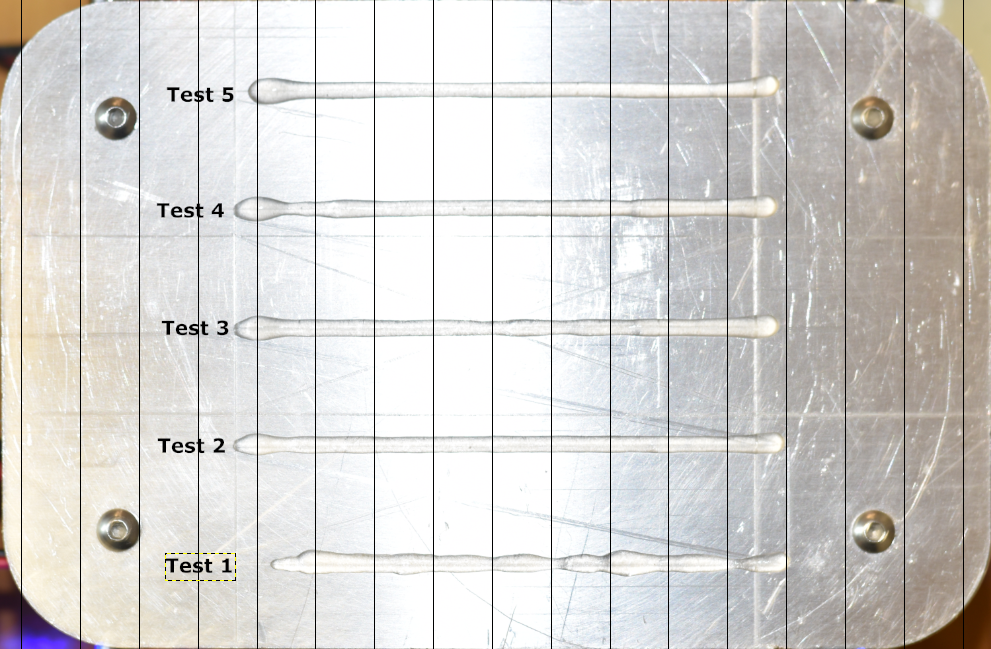
\includegraphics[width=0.6\textwidth]{figs/Phase_1.png}
    \caption{Trial 1 — nozzle height test}
    \label{fig:phase1}
\end{figure}

\begin{figure}[H]
    \centering
    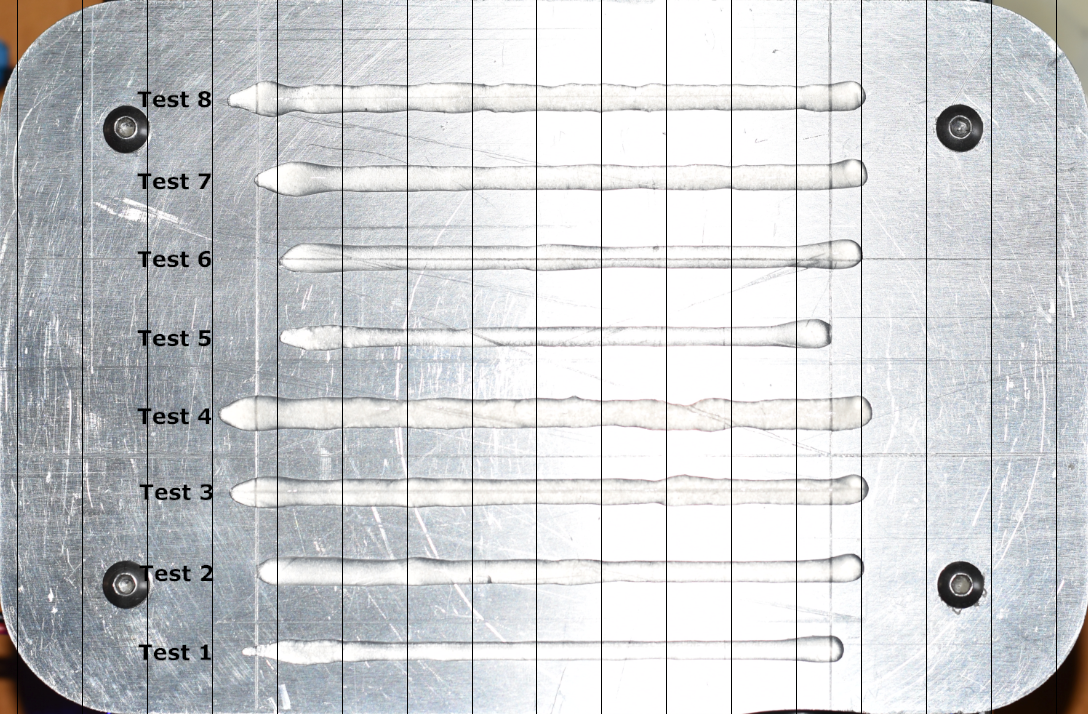
\includegraphics[width=0.6\textwidth]{figs/Phase_2a.png}
    \caption{Trial 2a — straight line test}
    \label{fig:phase2a}
\end{figure}

\begin{figure}[H]
    \centering
    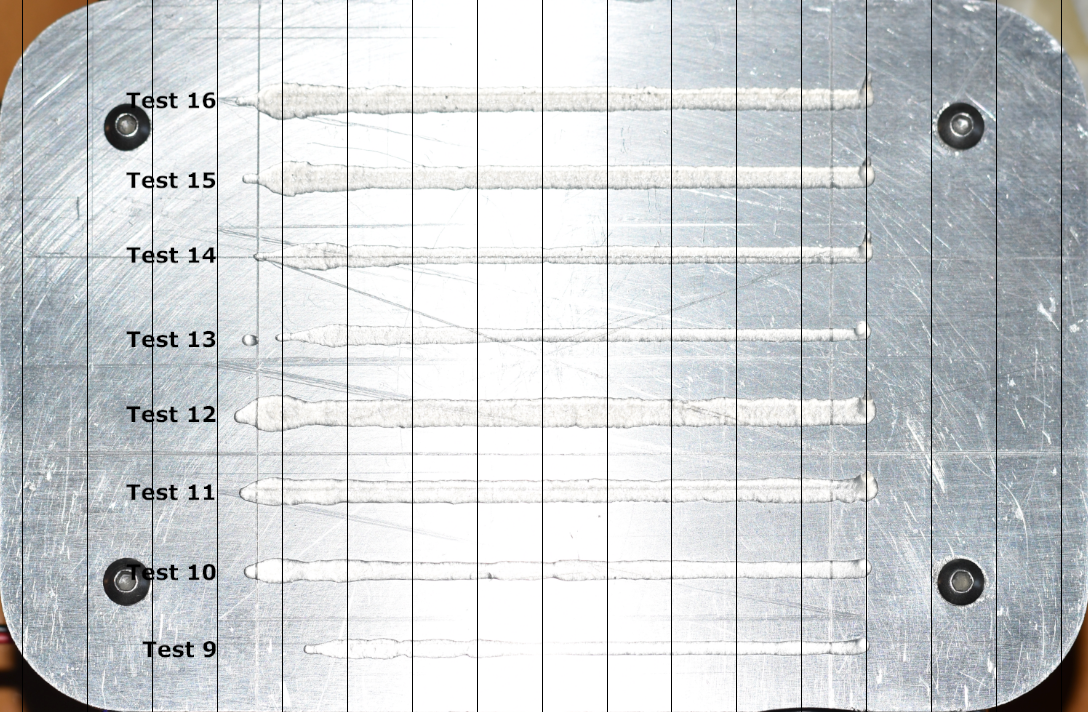
\includegraphics[width=0.6\textwidth]{figs/Phase_2b.png}
    \caption{Trial 2b — straight line test}
    \label{fig:phase2b}
\end{figure}

\begin{figure}[H]
    \centering
    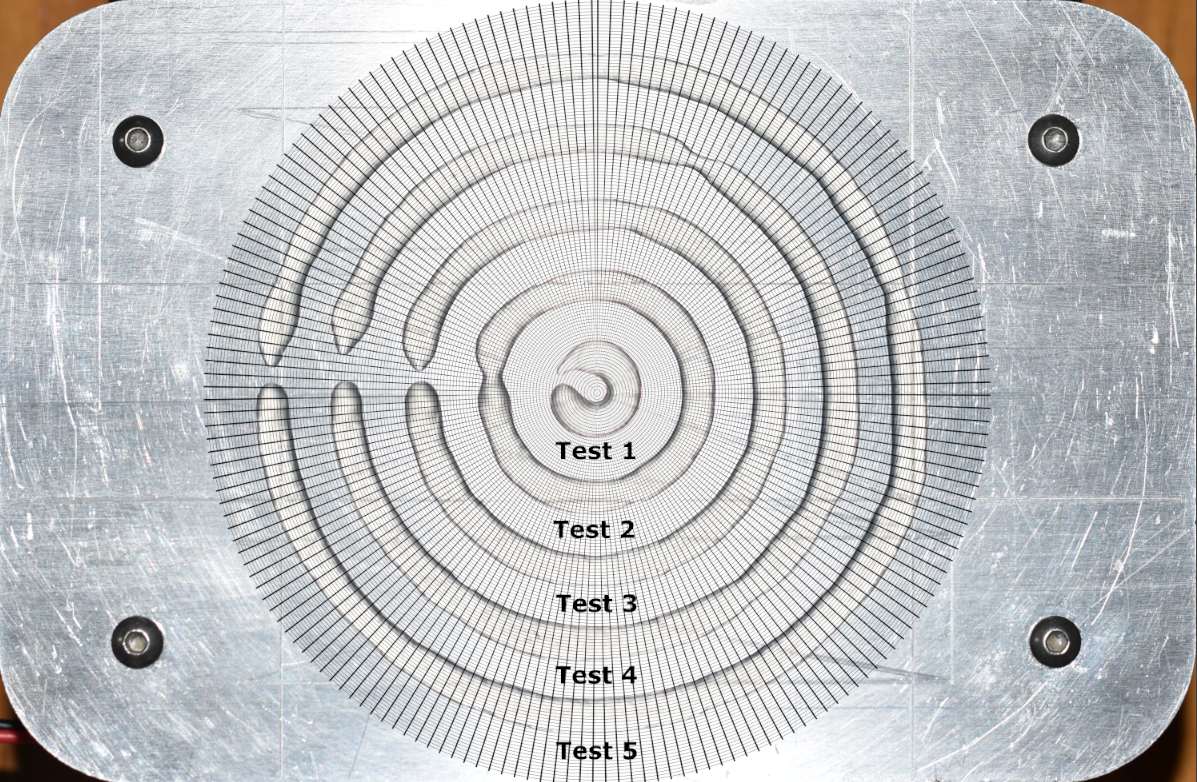
\includegraphics[width=0.6\textwidth]{figs/Phase_3.png}
    \caption{Trial 3 — circle test}
    \label{fig:phase3}
\end{figure}

\begin{figure}[H]
    \centering
    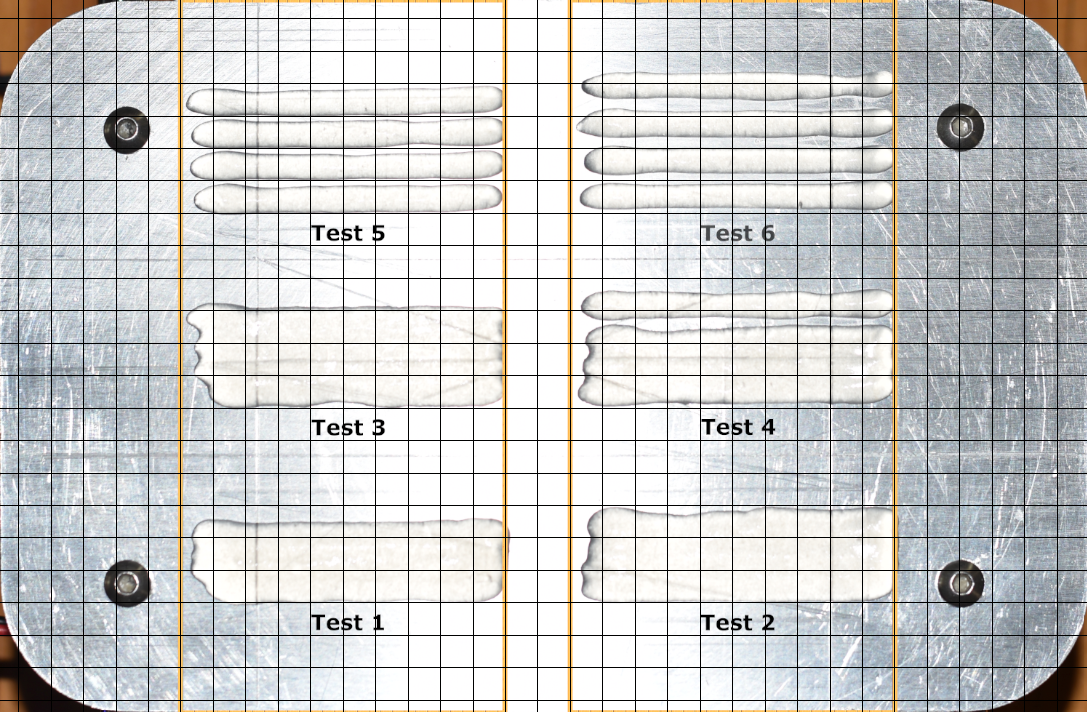
\includegraphics[width=0.6\textwidth]{figs/Phase_4.png}
    \caption{Trial 4 — adjacent lines test}
    \label{fig:phase4}
\end{figure}

\begin{figure}[H]
    \centering
    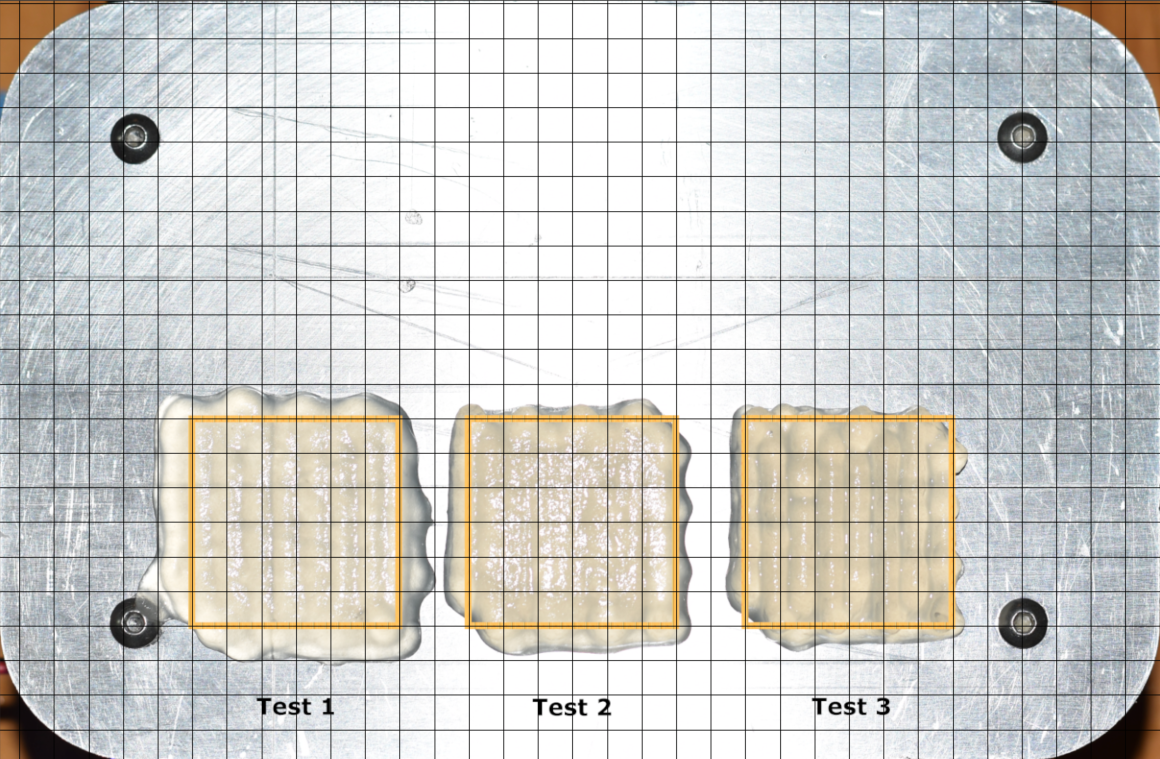
\includegraphics[width=0.6\textwidth]{figs/Phase_5a.png}
    \caption{Trial 5 — stacked layer test}
    \label{fig:phase5a}
\end{figure}
\begin{figure}[H]
    \centering
    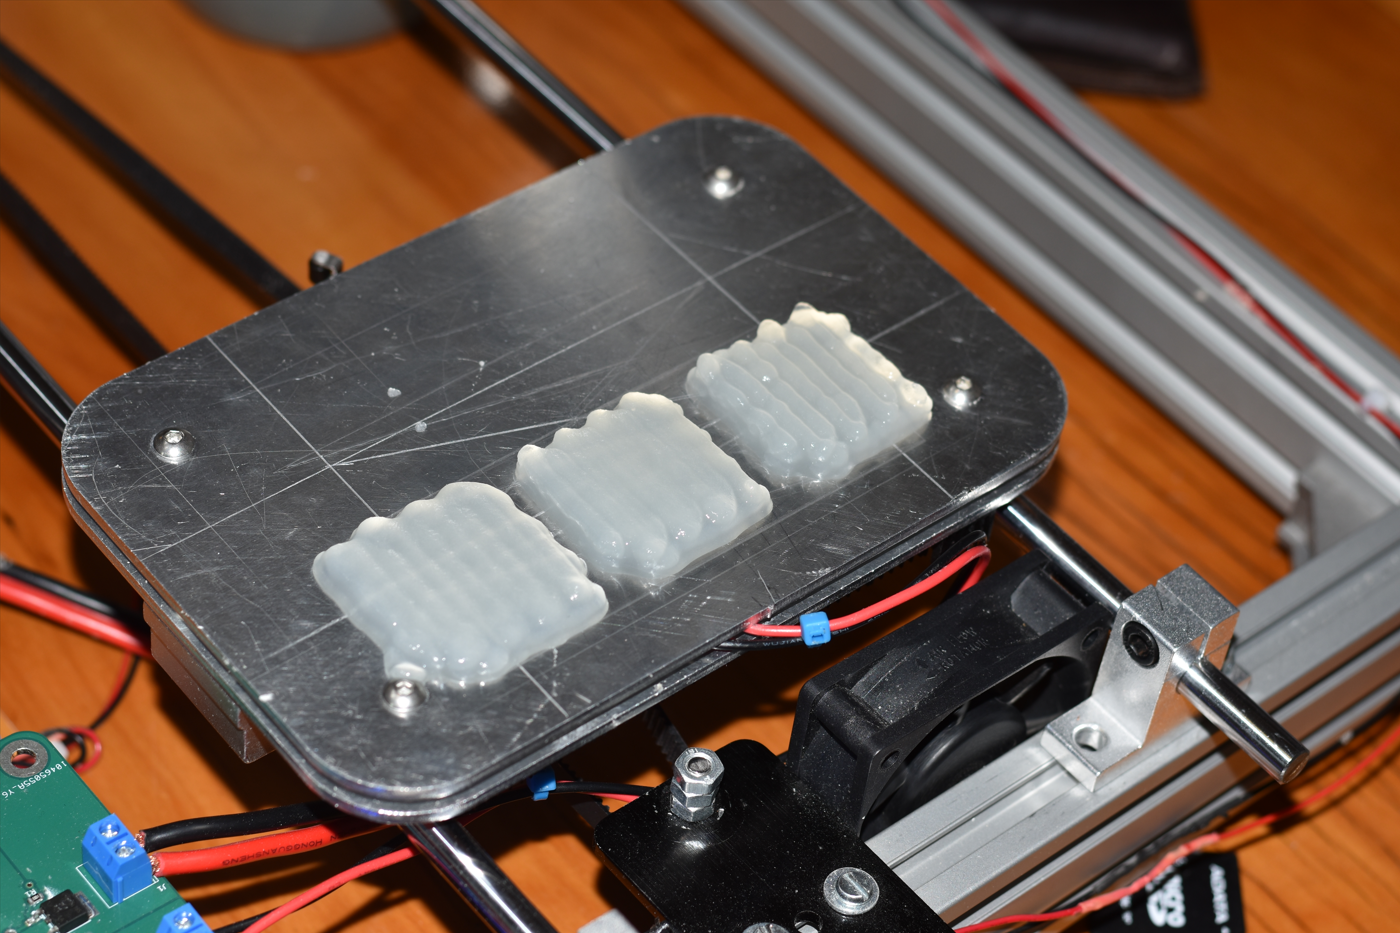
\includegraphics[width=0.6\textwidth]{figs/Phase_5b.png}
    \caption{Trial 5 — angled view}
    \label{fig:phase5b}
\end{figure}

\begin{figure}[H]
    \centering
    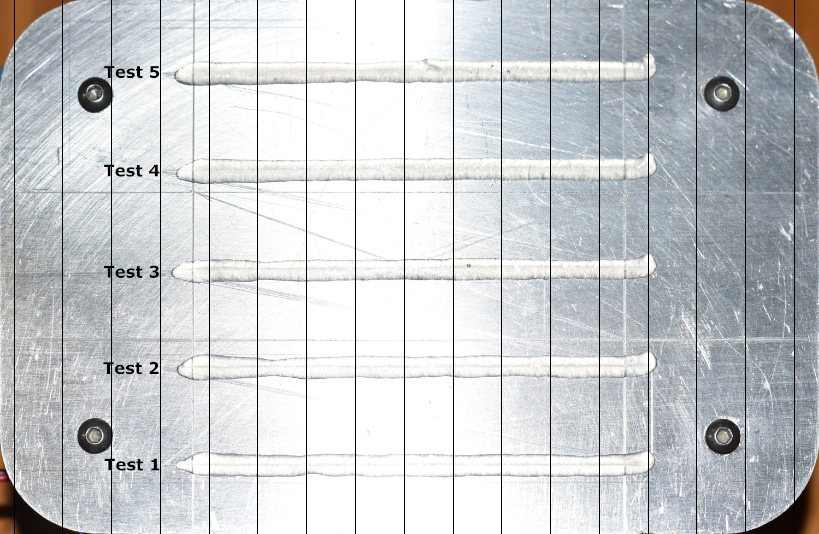
\includegraphics[width=0.6\textwidth]{figs/Phase_6.png}
    \caption{Trial 6 — repeatability test}
    \label{fig:phase6}
\end{figure}
\chapter{Techno-economic Analysis}
This section discusses the technical and economic aspects and impacts of the project. It covers time management, the project budget, technical impact, return on investment, and the project's potential for commercialisation.
\section{Planning and Time Management}
\begin{figure}[H]
    \centering
    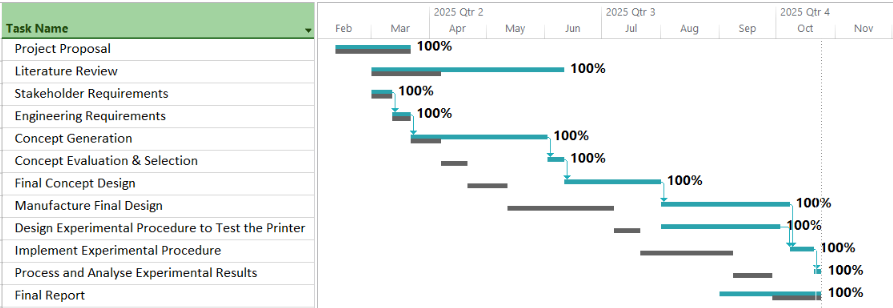
\includegraphics[width=\textwidth]{figs/ProjectGanttChart.png}
    \caption{Project Gantt Chart}
    \label{fig:gantt}
\end{figure}
The Gantt chart in Figure~\ref{fig:gantt} compares the predicted baseline duration (grey) of each project activity with the actual timeline (blue) in which the tasks were completed. It can be seen that the literature review extended over a significantly longer period than initially planned, due to the high workload from other modules during the first semester. A second major deviation occurred during the concept generation phase, which exceeded its planned duration because of an overly optimistic initial time estimate. The remaining project activities -- including completing the design process, manufacturing, assembling, and conducting the experimental work -- had to be completed within a shorter time frame to meet the final project deadline of 24~October~2025.

\section{Budget}
\begin{table}[H]
    \centering
    \caption{Estimated Project Budget}
    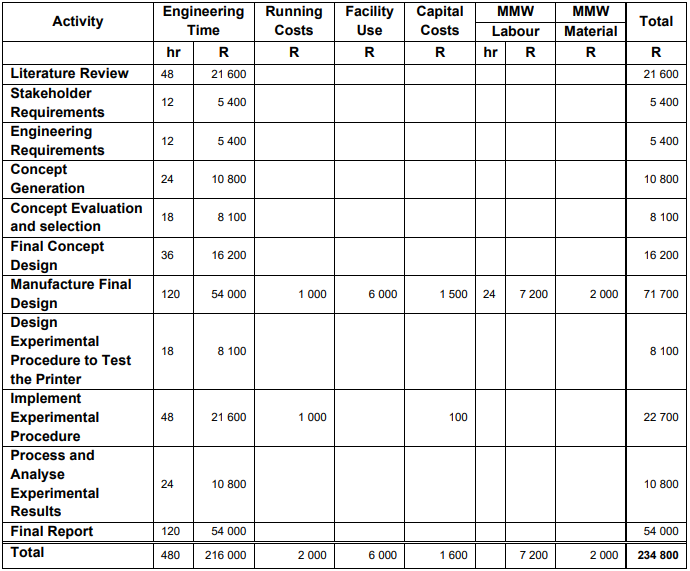
\includegraphics[width=0.8\textwidth]{figs/TheoreticalBudget.png}
    \label{tab:theoreticalBud}
\end{table}
\begin{table}[H]
    \centering
    \caption{Actual Project Cost}
    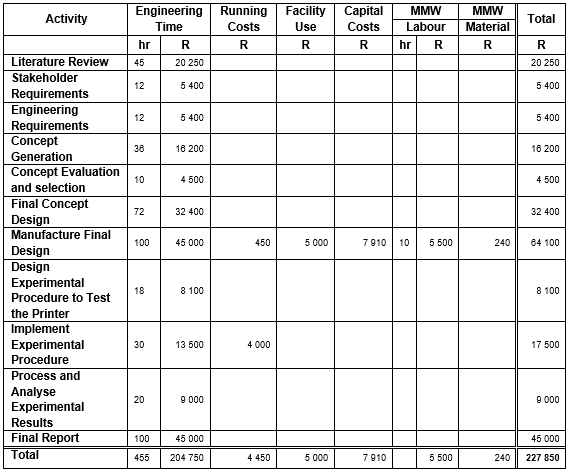
\includegraphics[width=0.8\textwidth]{figs/Actual Costs.png}
    \label{tab:actualCost}
\end{table}
The predicted budget and estimated final costs are shown in Tables~\ref{tab:theoreticalBud} and~\ref{tab:actualCost}. The actual cost of R227 850 was slightly below the initially predicted budget of R234 800. The largest discrepancies between the planned and actual expenses occurred in the running, capital, and workshop cost categories. These differences occurred because the final design was completed after the proposed budget had been estimated. Therefore, many required components that needed to be purchased or manufactured were not yet identified. In addition, the running cost estimate did not accurately account for electricity consumption and unplanned consumables such as lubricant.

The cost of component procurement, whether manufactured by the university or externally sourced, is summarised in Table~\ref{tab:costs}. This table reflects the total cost of developing the complete prototype, excluding the engineering time required for the system design.
\begin{table}[H]
    \centering
    \caption{Prototype Costs}
    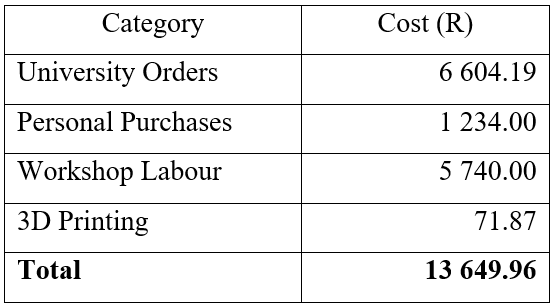
\includegraphics[width=0.5\textwidth]{figs/Costs.png}
    \label{tab:costs}
\end{table}

\section{Technical Impact}
The development of the hydrogel 3D printer provides a meaningful technical contribution to biomedical and tissue engineering research. The project demonstrates that repeatable hydrogel extrusion can be achieved using a cost-effective bioprinting system. On a technical level, the functional prototype serves as a flexible research tool for studying flow behaviour of unknown hydrogels. Building on the first iteration of this project -- done in 2024 -- this prototype integrates embedded control, modular hardware, and tunable parameters. It has also lowered the cost barrier for local tissue engineering research and established a stronger foundation for continued bioprinter development within the university.
\section{Return on Investment}
The time and money that was invested into this project resulted in a functional research platform. In the short term, the bioprinter serves as a means of characterising different unknown gels. In the long term, the system offers a low-cost alternative to imported high-cost bioprinters. Further development of this project by future students can refine the prototype into a laboratory-grade bioprinter with temperature control and closed-loop pressure feedback. The project therefore provides a high return on investment through its affordability, adaptability, and potential use as a research tool.
\section{Potential for Commercialization}
The project outcome is a functional prototype of a hydrogel 3D printer that shows potential for commercialization as an affordable and modular bioprinter for research institutions. Current commercial bioprinters, like the BIO X series, are not accessible for many laboratories due to their high costs, creating a market opportunity for more affordable alternatives. The open-source firmware and modular design makes the system adaptable to a wide range of hydrogels. With further refinement in sterility and addition of closed-loop syringe temperature and pressure control, an enclosure design, and user interface, the prototype can be developed to serve as a low-cost bioprinter for creating cell-laden scaffolds and characterising hydrogels for universities and other research institutions.
\chapter{Risk Analysis and Safety Procedures}
\section*{Safety Overview}
The mechanical and embedded system design, assembly and testing of the hydrogel 3D printer were performed at home, in a personal workspace, rather than in an official university laboratory or workshop. The project was conducted using a low-voltage electronic system and non-hazardous materials, and therefore presented minimal risks to both the user and equipment. Safety considerations, associated with the project, focused mainly on the mechanical, electrical, and thermal hazards associated with component assembly, soldering, and system handling.

The workspace was kept neat, tidy and ventilated to reduce the probability of tripping, remove solder fumes, and maintain easy access to equipment. Hazards such as the sharp edges of cut aluminium extrusions were eliminated by filing all edges after cutting. In cases where risks could not be completely eliminated, such as the presence of hot surfaces and nipping points, careful handling procedures were followed. This included keeping hands clear of the printer whenever in operation during the calibration stage and avoiding contact with heated components such as the nozzle and heat sinks until sufficient cooling time had elapsed after the printer was powered-down. To ensure the safe operation of the electronic system, protective measures were also implemented, such as limiting stepper driver current and verifying circuit connections with a multimeter before supplying power to the system.
\section*{Activity based Risk Assessment}
A risk assessment for the project is provided in Table~\ref{tab:risk}, which identifies the potential risks associated with each of project activity. The table also lists the corresponding steps to mitigate the likelihood and severity of each hazard to ensure personal safety (P) and equipment safety (E).
\begin{table}[H]
\centering
\caption{Risk assessment for the hydrogel 3D printer's development}
\label{tab:risk}
\begin{tabular}{|p{2.4cm}|p{3.3cm}|p{1cm}|p{6.0cm}|}
\hline
\textbf{Activity} & \textbf{Risk} & \textbf{Risk Type} & \textbf{Mitigating Steps} \\ \hline
Cutting aluminium & Cuts from sharp edges or saw blade & P & File all cut edges; clamp parts securely during cutting. \\ \hline
Assembling the printer & Thread stripping or cracking of 3D printed parts & E & Avoid over-tightening bolts. \\ \hline
Soldering & Burns and inhalation of fumes & P & Solder in a ventilated area; keep the iron in its stand when not in use. \\ \hline
PCB assembly & Short circuits & E & Verify polarity of components; test for continuity; avoid over-soldering joints. \\ \hline
Operating motors & Excessive current draw of drivers & E & Set current limits on stepper drivers. \\ \hline
Operating the printer & Pinch points between moving parts & P & Keep hands clear of moving parts during operation. \\ \hline
Hot surfaces & Burns from heated nozzle and heat sinks & P & Keep hands clear of heated parts during operation; allow adequate cooling time after power-down before handling. \\ \hline
Circuit handling & Static discharge & E & Disconnect power before handling PCB; ensure correct breakout driver orientation. \\ \hline
\end{tabular}
\end{table}

\chapter{Responsible Use of Resources and End-of-Life Strategy }
\section*{Responsible Use of Resources}
The hydrogel bioprinter was developed with the goal of using efficient materials and reusable components. The majority of the mechanical system consists of standard parts, including aluminium extrusions, TR8x8 lead screws, GT2 belts and pulleys, NEMA17 stepper motors, and linear bearings, which can all be reused in future student projects. 6 small PLA parts were 3D printed (4 feet and 2 limit switch mounts), resulting in minimal filament waste. The printer also includes several custom aluminium components (such as the syringe and bed plate) to ensure durability, most of which are made from aluminium plates to minimize machine waste.

The custom PCB was designed to maximise modularity, re-usability, and upgradability, by incorporating 5 stepper ports with breakout driver headers (StepStick form factor), 12 V switching ports, EEPROM storage, USB and SD card interface, and various breakout pins ensuring that the circuit board can be adapted across many different embedded systems applications. The experimental phase used store-bought agar powder as a hydrogel surrogate gel that is safe, biodegradable, inexpensive, and did not require a special disposal method.

\section*{End-of-Life Strategy}

At the end of the bioprinter's operational life, it can be disassembled into its mechanical and electronic components. The aluminium extrusions, motors, and other standard parts can be reused in future university projects or recycled through standard metal recycling facilities (along with the rest of the custom aluminium components). The PCB can be re-purposed to operate in other mechatronic systems or responsibly disposed of as electronic-waste and the PLA components can be recycled. The bioprinter’s modular design ensures that its components can be repaired, upgraded, or replaced, thereby extending the system's operational life and minimising environmental impact.

\backmatter%----------------------------------------------------------
\bibliography{bib/bib-sample}
\end{document}   

